% paper.tex -- MDPI journal paper
%DIF LATEXDIFF DIFFERENCE FILE
%DIF DEL docs/paper-v0/paper.tex   Fri May 29 11:56:02 2026
%DIF ADD paper/paper.tex           Fri May 29 12:57:38 2026
% Active Circuit Discovery: EFE-Guided Mechanistic Interpretability in LLMs
% Journal: Symmetry (MDPI) -- instructions: https://www.mdpi.com/journal/symmetry/instructions
% LaTeX template: https://www.mdpi.com/authors/latex
% Compiled with: pdflatex -> bibtex -> pdflatex -> pdflatex

\documentclass[symmetry,article,submit,pdftex,moreauthors]{Definitions/mdpi}

% =================================================================
% MDPI internal commands
\firstpage{1}
\makeatletter
\setcounter{page}{\@firstpage}
\makeatother
\pubvolume{1}
\issuenum{1}
\articlenumber{0}
\pubyear{2026}
\copyrightyear{2026}
%\datereceived{ }
%\daterevised{ }
%\dateaccepted{ }
%\datepublished{ }

% =================================================================
% Additional packages not in mdpi.cls
\usepackage{pgfplots}
\usetikzlibrary{shapes.geometric, shapes.misc, arrows.meta, positioning, fit,
                decorations.pathreplacing, calc, backgrounds,
                matrix, chains, scopes}
\usepgfplotslibrary{groupplots}
\pgfplotsset{compat=1.18}
\usepackage{adjustbox}

% Code listings
\lstset{
  basicstyle=\small\ttfamily,
  keywordstyle=\bfseries,
  commentstyle=\itshape,
  frame=single,
  breaklines=true,
  captionpos=b,
  numbers=left,
  numberstyle=\tiny,
  language=Python
}

% Theorem environments (defined in mdpi.cls, but custom ones needed)
\newtheorem{definition}{Definition}
\newtheorem{proposition}{Proposition}
\newtheorem{theorem}{Theorem}

% =================================================================
% Custom commands
\newcommand{\EFE}{\ensuremath{\mathcal{G}}}
\newcommand{\FE}{\ensuremath{\mathcal{F}}}
\newcommand{\KL}[2]{\ensuremath{D_{\mathrm{KL}}\!\left(#1 \,\|\, #2\right)}}
\newcommand{\E}[1]{\ensuremath{\mathbb{E}\!\left[#1\right]}}
\newcommand{\softmax}{\ensuremath{\operatorname{softmax}}}
\newcommand{\Attn}{\ensuremath{\operatorname{Attn}}}
\newcommand{\MLP}{\ensuremath{\operatorname{MLP}}}
\newcommand{\argmin}{\ensuremath{\operatorname*{arg\,min}}}
\newcommand{\abs}[1]{\ensuremath{\left|#1\right|}}
\newcommand{\norm}[1]{\ensuremath{\left\|#1\right\|}}
\newcommand{\vect}[1]{\ensuremath{\bm{#1}}}
\newcommand{\mat}[1]{\ensuremath{\mathbf{#1}}}
\newcommand{\ACDC}{ACDC}
\newcommand{\EAP}{EAP}
\newcommand{\ACD}{ACD}
\newcommand{\pymdp}{\texttt{pymdp}}

% =================================================================
% MDPI metadata (before \begin{document})

\Title{Active Circuit Discovery: A Multi-Action POMDP Agent
       for Causal Feature Identification\\in Transformer Attribution Graphs}

%DIF 78-80c78
%DIF < \newcommand{\orcidauthorA}{0000-0000-0000-000x}
%DIF < \newcommand{\orcidauthorB}{0000-0000-0000-000x}
%DIF < \newcommand{\orcidauthorC}{0000-0002-2671-0516}
%DIF -------
\newcommand{\orcidauthorA}{0000-0000-0000-000X} %DIF > 
%DIF -------

%DIF 82a80
\Author{Sharath Sathish $^{1}$\orcidA{}, Mominul Ahsan $^{2}$\orcidA{} and Majid Latifi $^{2,}$*\orcidA{}} %DIF > 
%DIF -------

%DIF 83-84d82
%DIF < \Author{Sharath Sathish $^{1}$\orcidA{}, Mominul Ahsan $^{2}$\orcidB{} and Majid Latifi $^{2,}$*\orcidC{}}
%DIF < 
%DIF -------
\AuthorNames{Sharath Sathish, Mominul Ahsan and Majid Latifi}

\address{%
$^{1}$ \quad BP International Limited, London TW16 7BP, UK; sharath.sathish@gmail.com \\
$^{2}$ \quad Department of Computer Science, University of York, York YO10 5GH, UK; mominul.ahsan2@gmail.com; majid.latifi@york.ac.uk}

\corres{majid.latifi@york.ac.uk}

\abstract{Mechanistic interpretability seeks to reverse-engineer the computational
%DIF 94-124c91-129
%DIF < circuits within large language models, yet current methods rely on
%DIF < exhaustive or heuristic search over exponentially many feature
%DIF < interactions. This paper introduces \emph{Active Circuit Discovery}
%DIF < (\ACD{}), a framework that combines attribution graph analysis with
%DIF < active inference for efficient circuit discovery. The framework
%DIF < integrates Anthropic's \texttt{circuit-tracer} library as the
%DIF < attribution graph backend, using Edge Attribution Patching with
%DIF < transcoders to identify active transcoder features per prompt.
%DIF < A POMDP agent, implemented with \texttt{pymdp}, maintains a
%DIF < multi-factor generative model of feature importance, layer role,
%DIF < and causal influence, and selects both the target feature and
%DIF < intervention type (ablation, activation patching, or feature
%DIF < steering) at each step by minimising Expected Free Energy over the
%DIF < joint feature--action space. The agent learns its observation model
%DIF < online through Dirichlet parameter updates, enabling principled
%DIF < exploration--exploitation trade-offs in circuit discovery.
%DIF < The framework is evaluated on two architectures, Gemma-2-2B (26 layers)
%DIF < and Llama-3.2-1B (16 layers), across four settings: Indirect Object
%DIF < Identification (IOI), multi-step reasoning, feature steering, and a
%DIF < multi-domain benchmark spanning geography, mathematics, science, logic,
%DIF < and history. With a budget of 20 interventions per prompt, the POMDP
%DIF < agent achieves 1255\% oracle efficiency on Gemma IOI and 90.6\% on
%DIF < Llama IOI, substantially outperforming random, greedy, and bandit
%DIF < baselines on both architectures.
%DIF < Feature steering confirms causal controllability: scaling individual
%DIF < features at $10\times$ activation changes predictions for 24 of 200
%DIF < tested features across both models ($p < 10^{-15}$, binomial test).
%DIF < Multi-domain analysis reveals task-dependent circuit structure: IOI
%DIF < circuits concentrate in late layers, while reasoning and scientific
%DIF < knowledge recruit early and middle layers.
%DIF < Code, notebooks, and experiment results are publicly available.
%DIF -------
circuits within large language models, but current methods rely on exhaustive %DIF > 
or heuristic search over exponentially many feature interactions. This paper %DIF > 
introduces \emph{Active Circuit Discovery} (\ACD{}), a framework that combines %DIF > 
attribution-graph analysis with active inference to select interventions %DIF > 
efficiently. \ACD{} uses Anthropic's \texttt{circuit-tracer} library as its %DIF > 
attribution-graph backend, applying Edge Attribution Patching with transcoders %DIF > 
to identify the active transcoder features for each prompt. A partially %DIF > 
observable Markov decision process (POMDP) agent, implemented with %DIF > 
\texttt{pymdp}, maintains a multi-factor generative model of feature %DIF > 
importance, layer role, and causal influence. At each step the agent selects %DIF > 
both a target feature and an intervention type (ablation, activation patching, %DIF > 
or feature steering) by minimising Expected Free Energy over the joint %DIF > 
feature--action space, and it learns its observation model online through %DIF > 
Dirichlet parameter updates. \ACD{} is an intervention-selection layer over %DIF > 
existing attribution-graph tools; it is not a whole-circuit discovery method, %DIF > 
and no claim of state-of-the-art circuit discovery is made. The framework is %DIF > 
evaluated on Gemma-2-2B (26 layers) and Llama-3.2-1B (16 layers) across four %DIF > 
settings: Indirect Object Identification (IOI), multi-step reasoning, feature %DIF > 
steering, and a multi-domain benchmark spanning geography, mathematics, %DIF > 
science, logic, and history. With a budget of 20 interventions per prompt, an %DIF > 
ablation-only agent scored by bounded oracle efficiency against the ablation %DIF > 
oracle reaches 82.0\% efficiency on Gemma IOI and 73.0\% on Gemma multi-step. %DIF > 
It exceeds random selection by 43.5 percentage points on Gemma IOI (paired %DIF > 
permutation $p=0.031$) and is competitive with greedy ranking, a heuristic UCB %DIF > 
bandit, and a plain UCB baseline. A direct Edge-Attribution-Patching ranking is %DIF > 
itself a strong baseline that the agent does not consistently surpass, and on %DIF > 
Llama multi-step the agent reaches 9.3\% efficiency (37.8\% with finer %DIF > 
layer-role bins). All comparisons report bootstrap 95\% confidence intervals. %DIF > 
The full multi-action agent is characterised separately by a \emph{Relative %DIF > 
Cumulative KL}, a steering-driven amplification factor reported apart from the %DIF > 
bounded efficiency. Feature steering changes the top-1 prediction in a %DIF > 
dose-dependent manner, but a matched random-feature control shows that %DIF > 
circuit-selected features are only marginally, and not significantly, more %DIF > 
steerable than random active features at large multipliers, indicating that %DIF > 
part of the effect is generic activation scaling. Multi-domain analysis shows %DIF > 
task-dependent circuit structure, with IOI circuits concentrated in late layers %DIF > 
and reasoning and scientific knowledge recruiting early and middle layers. Code, %DIF > 
notebooks (free T4), amd64/aarch64 Docker images, and raw results are publicly %DIF > 
available. %DIF > 
%DIF -------
}

%DIF 127c132
%DIF < \keyword{mechanistic interpretability; active inference; circuit discovery; transcoders; Expected Free Energy; POMDP agent}
%DIF -------
\keyword{mechanistic interpretability; active inference; circuit discovery; transcoders; Expected Free Energy; POMDP} %DIF > 
%DIF -------

% =================================================================
%DIF PREAMBLE EXTENSION ADDED BY LATEXDIFF
%DIF UNDERLINE PREAMBLE %DIF PREAMBLE
\RequirePackage[normalem]{ulem} %DIF PREAMBLE
\RequirePackage{color}\definecolor{RED}{rgb}{1,0,0}\definecolor{BLUE}{rgb}{0,0,1} %DIF PREAMBLE
\providecommand{\DIFadd}[1]{{\protect\color{blue}\uwave{#1}}} %DIF PREAMBLE
\providecommand{\DIFdel}[1]{{\protect\color{red}\sout{#1}}} %DIF PREAMBLE
%DIF SAFE PREAMBLE %DIF PREAMBLE
\providecommand{\DIFaddbegin}{} %DIF PREAMBLE
\providecommand{\DIFaddend}{} %DIF PREAMBLE
\providecommand{\DIFdelbegin}{} %DIF PREAMBLE
\providecommand{\DIFdelend}{} %DIF PREAMBLE
\providecommand{\DIFmodbegin}{} %DIF PREAMBLE
\providecommand{\DIFmodend}{} %DIF PREAMBLE
%DIF FLOATSAFE PREAMBLE %DIF PREAMBLE
\providecommand{\DIFaddFL}[1]{\DIFadd{#1}} %DIF PREAMBLE
\providecommand{\DIFdelFL}[1]{\DIFdel{#1}} %DIF PREAMBLE
\providecommand{\DIFaddbeginFL}{} %DIF PREAMBLE
\providecommand{\DIFaddendFL}{} %DIF PREAMBLE
\providecommand{\DIFdelbeginFL}{} %DIF PREAMBLE
\providecommand{\DIFdelendFL}{} %DIF PREAMBLE
%DIF COLORLISTINGS PREAMBLE %DIF PREAMBLE
\RequirePackage{listings} %DIF PREAMBLE
\RequirePackage{color} %DIF PREAMBLE
\lstdefinelanguage{DIFcode}{ %DIF PREAMBLE
%DIF DIFCODE_UNDERLINE %DIF PREAMBLE
  moredelim=[il][\color{red}\sout]{\%DIF\ <\ }, %DIF PREAMBLE
  moredelim=[il][\color{blue}\uwave]{\%DIF\ >\ } %DIF PREAMBLE
} %DIF PREAMBLE
\lstdefinestyle{DIFverbatimstyle}{ %DIF PREAMBLE
	language=DIFcode, %DIF PREAMBLE
	basicstyle=\ttfamily, %DIF PREAMBLE
	columns=fullflexible, %DIF PREAMBLE
	keepspaces=true %DIF PREAMBLE
} %DIF PREAMBLE
\lstnewenvironment{DIFverbatim}[1][]{\lstset{style=DIFverbatimstyle}}{} %DIF PREAMBLE
\lstnewenvironment{DIFverbatim*}[1][]{\lstset{style=DIFverbatimstyle,showspaces=true}}{} %DIF PREAMBLE
\lstset{extendedchars=\true,inputencoding=utf8}

%DIF END PREAMBLE EXTENSION ADDED BY LATEXDIFF

\begin{document}

\maketitle

% =================================================================
\section{Introduction}
\label{sec:intro}
% ---- introduction.tex ----

The rapid growth in the scale and deployment of large language models (LLMs) has
intensified the need for principled methods to audit, explain, and predict their
behaviour~\cite{Bereska2024}. Mechanistic interpretability pursues this goal by
reverse-engineering the internal computations of trained models into human-legible
circuits~\cite{Olah2020,Elhage2021}. A circuit, in this context, denotes the minimal
subgraph of model components (attention heads, MLP neurons, or SAE features) whose
activations are jointly necessary and sufficient to reproduce a specific model
behaviour on a given family of inputs~\cite{Cammarata2020,Wang2022}.

Circuit analysis has produced landmark findings. Wang et al.\ \DIFdelbegin \DIFdel{~\mbox{%DIFAUXCMD
\cite{Wang2022} }\hskip0pt%DIFAUXCMD
}\DIFdelend identified a
26-head circuit mediating Indirect Object Identification (IOI) in GPT-2
Small\DIFaddbegin \DIFadd{~\mbox{%DIFAUXCMD
\cite{Wang2022}}\hskip0pt%DIFAUXCMD
}\DIFaddend ; Hanna et al.\ \DIFdelbegin \DIFdel{~\mbox{%DIFAUXCMD
\cite{Hanna2023} }\hskip0pt%DIFAUXCMD
}\DIFdelend localised a circuit for numerical
greater-than comparisons\DIFaddbegin \DIFadd{~\mbox{%DIFAUXCMD
\cite{Hanna2023}}\hskip0pt%DIFAUXCMD
}\DIFaddend ; and Nanda et al.\ \DIFdelbegin \DIFdel{~\mbox{%DIFAUXCMD
\cite{Nanda2023Grokking} }\hskip0pt%DIFAUXCMD
}\DIFdelend traced the emergence of
modular arithmetic generalisation through a Fourier-space circuit during
grokking\DIFaddbegin \DIFadd{~\mbox{%DIFAUXCMD
\cite{Nanda2023Grokking}}\hskip0pt%DIFAUXCMD
}\DIFaddend . Each of these studies required thousands of
manually guided interventions, prompting interest in automation~\cite{Conmy2023,Syed2023}.

Automated Circuit \DIFdelbegin \DIFdel{DisCovery }\DIFdelend \DIFaddbegin \DIFadd{Discovery }\DIFaddend (\ACDC)~\cite{Conmy2023} generalises the activation
patching methodology of Wang et al.\ to a greedy graph-pruning algorithm that
systematically tests every edge in the computational graph. Although \ACDC\ achieves
strong fidelity on the IOI task, the number of interventions scales as $O(E)$ in the
number of graph edges, which for deep transformer models reaches the tens of
thousands. Edge Attribution Patching (\EAP)~\cite{Syed2023} reduces this cost by
approximating patch effects with integrated gradients, yet it trades correctness for
efficiency and may miss higher-order interactions. Neither method incorporates
uncertainty about the circuit structure or adapts its search strategy based on what
has already been discovered.

\DIFdelbegin \DIFdel{Novelty of }\DIFdelend \DIFaddbegin \DIFadd{The novelty of this work lies in an }\DIFaddend uncertainty-guided \DIFdelbegin \DIFdel{adaptive search}\DIFdelend \DIFaddbegin \DIFadd{intervention-selection
layer, not in a new attribution backend. \ACD{} is not a replacement for
attribution-graph construction methods such as \EAP{} or }\texttt{\DIFadd{circuit-tracer}}\DIFadd{;
it consumes their output, a pruned attribution graph over transcoder features, and
contributes a policy for choosing which feature to intervene on next, and how, under
a fixed intervention budget. The novelty therefore lies in the adaptive search
strategy rather than in how the candidate graph is built}\DIFaddend .
To date, \DIFaddbegin \DIFadd{automated }\DIFaddend circuit discovery has pursued either exhaustive search (as in
\ACDC) or gradient-based ranking (as in \EAP \DIFdelbegin \DIFdel{\ }\DIFdelend and Causal Tracing~\cite{Meng2022}),
with Sparse Feature Circuits~\cite{marks2024sparse} and Dictionary Learning
approaches~\cite{He2024} following similar gradient-plus-pruning paradigms. None of
these methods explicitly maintains a belief distribution over circuit components or
uses uncertainty to guide adaptive, budget-aware exploration. This \DIFdelbegin \DIFdel{presents a significant practical
challenge: while production systems operate under strict computational constraints, current methodologies fail to optimise the informativeness of individual interventions }\DIFdelend \DIFaddbegin \DIFadd{poses a practical
problem: in production systems the number of interventions is constrained by
compute budgets, yet existing methods do not optimise for informativeness per
intervention}\DIFaddend . The statistical literature on active learning and Bayesian experimental
design~\cite{MacKay2003} has long established that uncertainty-guided selection
outperforms passive ranking when the goal is to resolve ambiguity with minimal
queries. The present work brings this principle to circuit discovery: by formulating
the problem as a Partially Observable Markov Decision Process (POMDP) and selecting
interventions to minimise Expected Free Energy (EFE), the framework achieves
information-theoretically principled adaptation that trades off exploration
(resolving circuit uncertainty) with exploitation (confirming known important
features).

Active Inference is a normative framework for perception and action in biological
agents that unifies perception, learning, and planning under a single objective\DIFdelbegin \DIFdel{of minimising }\DIFdelend \DIFaddbegin \DIFadd{: the
minimisation of }\DIFaddend variational free energy \DIFdelbegin \DIFdel{, which is equivalent to maximising model
evidence}\DIFdelend \DIFaddbegin \DIFadd{(equivalently, the maximisation of model
evidence)}\DIFaddend ~\cite{Friston2010,Parr2022}. When extended to planning, the framework
introduces the Expected Free Energy (\EFE), which decomposes into an epistemic term
(expected information gain about hidden states) and a pragmatic term (expected
alignment with preferences)~\cite{Friston2015,DaCosta2020}. \DIFdelbegin \DIFdel{The minimization of }\DIFdelend \EFE\
\DIFdelbegin \DIFdel{naturally balances the trade-off between }\DIFdelend \DIFaddbegin \DIFadd{minimisation naturally trades off }\DIFaddend exploration and exploitation\DIFdelbegin \DIFdel{, as the agent prioritises actions that simultaneously reduce environmental uncertainty and advance the attainment of preferred }\DIFdelend \DIFaddbegin \DIFadd{: an agent selects
actions that resolve uncertainty about the world while pursuing desired }\DIFaddend outcomes.

This work proposes that circuit discovery is precisely the kind of problem for which
\EFE\ minimisation is appropriate. The ``world'' is the causal graph of an LLM; the
``actions'' are ablation and activation-patching interventions; the ``hidden states''
are the identities and importances of circuit-critical features; and the ``preference''
is the rapid identification of a faithful, minimal circuit. An Active Inference agent
that maintains a belief distribution over candidate circuit components and selects
interventions to maximally resolve that uncertainty will, in theory, identify circuits
with fewer total interventions than either random or gradient-ranked selection.

The contributions of this paper are as follows.

\emph{(C1) Active Inference formulation.} Circuit discovery is cast as a
partially observable Markov decision process \DIFaddbegin \DIFadd{(POMDP) }\DIFaddend with three hidden state
factors (feature importance, layer role, causal influence), three observation
modalities (KL divergence, activation magnitude, graph connectivity), and three
actions (ablation, patching, steering). The agent is implemented using the
\texttt{pymdp} library~\cite{Pymdp2022}, with Expected Free Energy guiding
intervention selection and Dirichlet parameter updates enabling online learning
of the observation model.

\emph{(C2) Framework implementation.} The \DIFdelbegin \DIFdel{\ACD\
}\DIFdelend \DIFaddbegin \DIFadd{Active Circuit Discovery (\ACD)
}\DIFaddend framework integrates Anthropic's
\texttt{circuit-tracer}~\cite{Anthropic2025CT,Ameisen2025} for Edge Attribution Patching
with GemmaScope transcoders and the \texttt{feature\_intervention} API for
causally correct transcoder-level interventions.

\emph{(C3) Validated evaluation \DIFaddbegin \DIFadd{with action-matched and attribution baselines}\DIFaddend .}
The \DIFdelbegin \DIFdel{POMDP }\DIFdelend agent is compared against a heuristic bandit\DIFdelbegin \DIFdel{baseline}\DIFdelend , greedy importance ranking, \DIFaddbegin \DIFadd{a
direct Edge-Attribution-Patching (\EAP) ranking baseline computed from
}\texttt{\DIFadd{circuit-tracer}} \DIFadd{attribution scores, }\DIFaddend random selection, and an oracle upper
bound\DIFaddbegin \DIFadd{, }\DIFaddend on two models (Gemma-2-2B \DIFdelbegin \DIFdel{~\mbox{%DIFAUXCMD
\cite{team2024gemma}
}\hskip0pt%DIFAUXCMD
}\DIFdelend and Llama-3.2-1B\DIFdelbegin \DIFdel{~\mbox{%DIFAUXCMD
\cite{Dubey2024llama}}\hskip0pt%DIFAUXCMD
}\DIFdelend ) across four benchmarks (IOI,
multi-step reasoning, feature steering, and a five-domain cognitive benchmark).
\DIFaddbegin \DIFadd{To isolate the contribution of selection from that of the intervention
type, an ablation-only agent (POMDP-abl) is evaluated against the ablation
oracle as the primary, fair comparison, and action-matched
(steering-enabled) variants of the random, greedy, and bandit baselines are reported
separately. A plain UCB baseline is also included to isolate the heuristic bandit's
engineered inductive bias.
}\DIFaddend 

\DIFdelbegin \emph{\DIFdel{(C4) Causal controllability.}} %DIFAUXCMD
\DIFdel{Featureis the uncertainty bonus (initialised to 1, decayed on visit) and steering experiments demonstrate
that individual transcoder features causally control model behaviour, with
prediction changes observed at $10\times$ activation scaling .
}\DIFdelend \DIFaddbegin \emph{\DIFadd{(C4) Causal controllability, with controls.}} \DIFadd{Feature steering experiments
show that scaling transcoder features changes predictions in a clear dose-dependent
manner, far above chance. A random-feature control reveals that
circuit-selected features are only marginally, and not significantly, more
steerable than randomly chosen features at large multipliers, indicating that a
substantial part of the effect is generic activation scaling rather than
selection-specific causal control. The causal claim is therefore stated cautiously
and the controls are reported in full.
}\DIFaddend 

\emph{(C5) Reproducibility artifacts.} Three Google Colab notebooks \DIFaddbegin \DIFadd{(free T4 GPU),
both an aarch64 (DGX Spark) and a standard }\texttt{\DIFadd{x86\_64}}\DIFadd{/amd64 Docker image}\DIFaddend , \DIFdelbegin \DIFdel{a Docker
container for NVIDIA DGX Spark, }\DIFdelend and
raw experiment results (JSON) are released for full reproduction.

\DIFdelbegin \DIFdel{Positioning statement. }\DIFdelend To the best of the authors' knowledge, this is the first
work to cast circuit discovery as a POMDP with principled Expected Free Energy
\DIFdelbegin \DIFdel{minimization }\DIFdelend \DIFaddbegin \DIFadd{minimisation }\DIFaddend for uncertainty-guided adaptive intervention selection. Prior work has
not combined \DIFdelbegin \DIFdel{(a) }\DIFdelend uncertainty-aware feature importance estimation via \DIFdelbegin \DIFdel{belief state
evolution, (b) }\DIFdelend \DIFaddbegin \DIFadd{belief-state
evolution, }\DIFaddend a multi-action intervention space with learnable action-type
selection, \DIFdelbegin \DIFdel{(c) online generative model }\DIFdelend \DIFaddbegin \DIFadd{online generative-model }\DIFaddend learning via Dirichlet posterior updates,
and \DIFdelbegin \DIFdel{(d) }\DIFdelend transcoder-level causal interventions across the full feature space. These
components together \DIFdelbegin \DIFdel{enable significantly more sample-efficient circuit discovery than exhaustive or gradient-based approaches. }\DIFdelend \DIFaddbegin \DIFadd{constitute a previously unexplored design
point for the intervention-selection sub-problem. No claim is made of
state-of-the-art circuit discovery relative to \ACDC{} or \EAP{}. On a shared
attribution-graph backend and a fixed budget, EFE-guided selection (POMDP-abl)
reliably beats random selection and is competitive with greedy, a heuristic UCB
bandit, and a plain UCB baseline; a direct \EAP{} attribution ranking is itself a
strong ablation-KL baseline and is not consistently beaten
(Section~\ref{sec:results}). The agent's distinctive value is therefore the explicit
belief-state uncertainty, the multi-action space, and online model learning,
capabilities the static baselines lack, rather than a raw efficiency win.
}\DIFaddend 

The following testable hypotheses guide the evaluation.

\emph{H1 (Efficiency).}  The POMDP agent\DIFaddbegin \DIFadd{, restricted to the ablation
action for a fair comparison (the ablation-only variant ``POMDP-abl''),
}\DIFaddend identifies causally important features with higher cumulative KL
divergence than random selection within a fixed budget of $B=20$
interventions. \DIFdelbegin \DIFdel{Assessed }\DIFdelend \DIFaddbegin \DIFadd{This is assessed }\DIFaddend via a one-sided paired $t$-test \DIFaddbegin \DIFadd{and an exact
one-sided paired permutation test }\DIFaddend across prompts ($\alpha = 0.05$)\DIFaddbegin \DIFadd{, with the
permutation test treated as primary given the small prompt counts}\DIFaddend .

\emph{H2 (Causal controllability).}  \DIFdelbegin \DIFdel{Scaling individual transcoder features at $10\times$ activation }\DIFdelend \DIFaddbegin \DIFadd{This hypothesis comprises two sub-claims.
Under H2a (manipulability), scaling transcoder features }\DIFaddend changes the
model's top-1 prediction \DIFdelbegin \DIFdel{for a non-trivial fraction of features. Assessed via a }\DIFdelend \DIFaddbegin \DIFadd{far above chance, in a dose-dependent manner
across the multiplier sweep (}\DIFaddend one-sided binomial test against a 1\%
\DIFdelbegin \DIFdel{chance-level baseline(}\DIFdelend \DIFaddbegin \DIFadd{chance baseline). Under H2b (selectivity), circuit-selected features
are more controllable than matched randomly chosen features
(one-sided Fisher exact test of selected versus control flip rates,
}\DIFaddend $\alpha = 0.05$). \DIFaddbegin \DIFadd{Separating these sub-claims lets the controls reveal how
much of the steering effect is specific to selected features versus
generic activation scaling.
}\DIFaddend 

\emph{H3 (Discovery quality).}  The \DIFdelbegin \DIFdel{POMDP agent achieves oracle
efficiency }\DIFdelend \DIFaddbegin \DIFadd{ablation-only agent (POMDP-abl) recovers
}\DIFaddend $\geq 50\%$ \DIFaddbegin \DIFadd{of the ablation oracle's cumulative KL }\DIFaddend with budget $B=20$
\DIFaddbegin \DIFadd{(bounded oracle efficiency)}\DIFaddend . Assessed by point estimate \DIFdelbegin \DIFdel{and
standard deviation }\DIFdelend \DIFaddbegin \DIFadd{with a bootstrap
95\% confidence interval }\DIFaddend across prompts.

\emph{H4 (Cross-architecture transfer).}  The qualitative findings
obtained on Gemma-2-2B replicate on Llama-3.2-1B.

The remainder of this paper is structured as follows. Section~\ref{sec:background}
reviews related work on circuit analysis, active learning and Bayesian
experimental design, Active Inference, and sparse autoencoders. Section~\ref{sec:method}
describes the \ACD{} framework in detail. Section~\ref{sec:setup} specifies the
experimental protocol. Section~\ref{sec:results} reports validated results. Section~\ref{sec:discussion}
provides an expanded discussion of findings, limitations, and future directions. Section~\ref{sec:conclusion}
concludes\DIFdelbegin \DIFdel{and discusses future work}\DIFdelend . Additional implementation details and supplementary analyses are provided
in the Appendix.


% =================================================================
\section{Background and Related Work}
\label{sec:background}
% ---- background.tex ----

\subsection{Mechanistic Interpretability and Circuit Analysis}

Mechanistic interpretability traces causal pathways through neural networks by
applying targeted interventions (zeroing activations, swapping activations between
forward passes on different inputs, or replacing specific components with learned
approximations) and measuring the resulting change in model output~\cite{Pearl2009,
Geiger2021}. The transformer architecture~\cite{Vaswani2017} is especially amenable to
this analysis because its residual stream structure allows the contribution of each
component to the final logits to be decomposed additively~\cite{Elhage2021}.

Olah et al.\ \DIFdelbegin \DIFdel{~\mbox{%DIFAUXCMD
\cite{Olah2020,Cammarata2020} }\hskip0pt%DIFAUXCMD
}\DIFdelend introduced the concept of circuits in convolutional vision
networks\DIFaddbegin \DIFadd{~\mbox{%DIFAUXCMD
\cite{Olah2020,Cammarata2020}}\hskip0pt%DIFAUXCMD
}\DIFaddend . Elhage et al.\ \DIFdelbegin \DIFdel{~\mbox{%DIFAUXCMD
\cite{Elhage2021} }\hskip0pt%DIFAUXCMD
}\DIFdelend formalised the residual stream
decomposition for transformers and demonstrated in-context learning heads, induction
heads, and name-mover heads in small two-layer models\DIFaddbegin \DIFadd{~\mbox{%DIFAUXCMD
\cite{Elhage2021}}\hskip0pt%DIFAUXCMD
}\DIFaddend . Wang et al.\
\DIFdelbegin \DIFdel{~\mbox{%DIFAUXCMD
\cite{Wang2022}
}\hskip0pt%DIFAUXCMD
}\DIFdelend applied this framework at scale in a celebrated study of the 26-head IOI circuit
in GPT-2 Small, using path patching to confirm causal roles\DIFaddbegin \DIFadd{~\mbox{%DIFAUXCMD
\cite{Wang2022}}\hskip0pt%DIFAUXCMD
}\DIFaddend . Subsequent
work characterised circuits for docstring completion~\cite{Heimersheim2023},
numerical reasoning~\cite{Hanna2023}, copy suppression in attention
heads~\cite{McDougall2023}, and Chinchilla at 70~B
parameters~\cite{Lieberum2023}.

A recurring limitation of manual circuit analysis is labour intensity. Conmy et al.\
\DIFdelbegin \DIFdel{~\mbox{%DIFAUXCMD
\cite{Conmy2023} }\hskip0pt%DIFAUXCMD
}\DIFdelend addressed this with \DIFdelbegin \DIFdel{ACDC}\DIFdelend \DIFaddbegin \DIFadd{Automated Circuit Discovery (\ACDC)}\DIFaddend , a greedy edge-pruning
algorithm that recovers circuits matching manual analyses on the IOI and docstring
tasks\DIFaddbegin \DIFadd{~\mbox{%DIFAUXCMD
\cite{Conmy2023}}\hskip0pt%DIFAUXCMD
}\DIFaddend . Syed et al.\ \DIFdelbegin \DIFdel{~\mbox{%DIFAUXCMD
\cite{Syed2023} }\hskip0pt%DIFAUXCMD
}\DIFdelend proposed Edge Attribution Patching (\EAP), which
approximates intervention effects with gradient-based attribution and achieves
competitive results at a fraction of the runtime\DIFaddbegin \DIFadd{~\mbox{%DIFAUXCMD
\cite{Syed2023}}\hskip0pt%DIFAUXCMD
}\DIFaddend . Geiger et al.\
\DIFdelbegin \DIFdel{~\mbox{%DIFAUXCMD
\cite{Geiger2021}
}\hskip0pt%DIFAUXCMD
}\DIFdelend introduced causal abstraction as a formal verification criterion for circuit
hypotheses\DIFaddbegin \DIFadd{~\mbox{%DIFAUXCMD
\cite{Geiger2021}}\hskip0pt%DIFAUXCMD
}\DIFaddend , and Chan et al.\ \DIFdelbegin \DIFdel{~\mbox{%DIFAUXCMD
\cite{Chan2022} }\hskip0pt%DIFAUXCMD
}\DIFdelend developed causal scrubbing for
the same purpose\DIFaddbegin \DIFadd{~\mbox{%DIFAUXCMD
\cite{Chan2022}}\hskip0pt%DIFAUXCMD
}\DIFaddend .

Meng et al.\ \DIFdelbegin \DIFdel{~\mbox{%DIFAUXCMD
\cite{Meng2022} }\hskip0pt%DIFAUXCMD
}\DIFdelend complemented circuit analysis with causal tracing applied to factual
associations in GPT models, identifying mid-layer MLP blocks as the primary locus of
stored world knowledge\DIFaddbegin \DIFadd{~\mbox{%DIFAUXCMD
\cite{Meng2022}}\hskip0pt%DIFAUXCMD
}\DIFaddend . Recent efforts have extended circuit analysis
to sparse autoencoders and transcoders: Marks et al.\ \DIFdelbegin \DIFdel{~\mbox{%DIFAUXCMD
\cite{marks2024sparse} }\hskip0pt%DIFAUXCMD
}\DIFdelend combined gradient-based pruning
with sparse features\DIFaddbegin \DIFadd{~\mbox{%DIFAUXCMD
\cite{marks2024sparse}}\hskip0pt%DIFAUXCMD
}\DIFaddend , while He et al.\ \DIFdelbegin \DIFdel{~\mbox{%DIFAUXCMD
\cite{He2024} }\hskip0pt%DIFAUXCMD
}\DIFdelend applied dictionary
learning to discover interpretable circuits\DIFaddbegin \DIFadd{~\mbox{%DIFAUXCMD
\cite{He2024}}\hskip0pt%DIFAUXCMD
}\DIFaddend . Lindsey et al.\ \DIFdelbegin \DIFdel{~\mbox{%DIFAUXCMD
\cite{Anthropic2025CT} }\hskip0pt%DIFAUXCMD
}\DIFdelend recently
combined attribution graphs constructed via \texttt{circuit-tracer}\DIFaddbegin \DIFadd{~\mbox{%DIFAUXCMD
\cite{Anthropic2025CT}
}\hskip0pt%DIFAUXCMD
}\DIFaddend with large-scale SAE analysis to map the biology of Claude~3 Sonnet at a component
level~\cite{Lindsey2025}.

\subsection{Sparse Autoencoders and Transcoders}

Polysemanticity, the tendency of individual neurons to respond to multiple unrelated
concepts, has been identified as a core obstacle to mechanistic
interpretability~\cite{Olah2020,Bricken2023}. Sparse Autoencoders (SAEs) address this
by learning an overcomplete, sparse linear basis for the residual stream at each layer.
Cunningham et al.\ \DIFdelbegin \DIFdel{~\mbox{%DIFAUXCMD
\cite{Cunningham2024} }\hskip0pt%DIFAUXCMD
}\DIFdelend demonstrated that features learned by SAEs are substantially more
monosemantic than individual neurons\DIFaddbegin \DIFadd{~\mbox{%DIFAUXCMD
\cite{Cunningham2024}}\hskip0pt%DIFAUXCMD
}\DIFaddend . Bricken et al.\ \DIFdelbegin \DIFdel{~\mbox{%DIFAUXCMD
\cite{Bricken2023} }\hskip0pt%DIFAUXCMD
}\DIFdelend scaled
this approach to a one-layer MLP with 4,096-dimensional activations, recovering over
512 interpretable features including curve detectors and orientation-selective
units\DIFaddbegin \DIFadd{~\mbox{%DIFAUXCMD
\cite{Bricken2023}}\hskip0pt%DIFAUXCMD
}\DIFaddend . Gao et al.\ \DIFdelbegin \DIFdel{~\mbox{%DIFAUXCMD
\cite{Gao2024} }\hskip0pt%DIFAUXCMD
}\DIFdelend studied scaling and evaluation of $k$-sparse SAEs at large scale,
including on {GPT-4} activations, and reported scaling laws for reconstruction
and feature quality\DIFaddbegin \DIFadd{~\mbox{%DIFAUXCMD
\cite{Gao2024}}\hskip0pt%DIFAUXCMD
}\DIFaddend .
Rajamanoharan et al.\ \DIFdelbegin \DIFdel{~\mbox{%DIFAUXCMD
\cite{Rajamanoharan2024} }\hskip0pt%DIFAUXCMD
}\DIFdelend proposed Gated Sparse Autoencoders, which improve feature
monosemanticity by decoupling feature detection from magnitude
estimation\DIFaddbegin \DIFadd{~\mbox{%DIFAUXCMD
\cite{Rajamanoharan2024}}\hskip0pt%DIFAUXCMD
}\DIFaddend . Paulo et al.\ \DIFdelbegin \DIFdel{~\mbox{%DIFAUXCMD
\cite{Paulo2024} }\hskip0pt%DIFAUXCMD
}\DIFdelend demonstrated large-scale automated
interpretation of millions of SAE features using large language models as
interpretability oracles\DIFaddbegin \DIFadd{~\mbox{%DIFAUXCMD
\cite{Paulo2024}}\hskip0pt%DIFAUXCMD
}\DIFaddend . Makelov et al.\ \DIFdelbegin \DIFdel{~\mbox{%DIFAUXCMD
\cite{Makelov2024} }\hskip0pt%DIFAUXCMD
}\DIFdelend provided principled evaluation criteria for
SAE quality, showing that standard metrics can overestimate
interpretability\DIFaddbegin \DIFadd{~\mbox{%DIFAUXCMD
\cite{Makelov2024}}\hskip0pt%DIFAUXCMD
}\DIFaddend .

Transcoders are a related architecture that decompose MLP input-to-output
transformations directly, providing a more causally faithful representation of MLP
computation than residual-stream SAEs. Anthropic's \texttt{circuit-tracer}
library~\cite{Anthropic2025CT,Ameisen2025} provides an end-to-end pipeline for
feature-level attribution: transcoders decompose MLP activations into sparse
features, and Edge Attribution Patching constructs a directed graph of feature
interactions.  The \texttt{feature\_intervention} API then allows causally correct
ablation and steering of individual transcoder features with proper network
propagation.  GemmaScope~\cite{team2024gemma,GemmaScope2024} provides pre-trained transcoders and
SAEs for Google's Gemma-2 model family, enabling open interpretability research at scale.

\subsection{Active Inference and Expected Free Energy}

Active Inference is a unified computational framework derived from the Free Energy
Principle~\cite{Friston2010}, which posits that biological agents minimise the
surprise (negative model log-evidence) associated with their sensory states. Friston
et al.\ \DIFdelbegin \DIFdel{~\mbox{%DIFAUXCMD
\cite{Friston2017} }\hskip0pt%DIFAUXCMD
}\DIFdelend formalised this as variational inference: agents approximate the true posterior
over hidden states $\vect{s}$ given observations $\vect{o}$ by maintaining a
recognition distribution $q(\vect{s})$ and minimising the variational free energy
$\FE = \KL{q(\vect{s})}{p(\vect{s}\mid\vect{o})} \geq
-\log p(\vect{o})$\DIFaddbegin \DIFadd{~\mbox{%DIFAUXCMD
\cite{Friston2017}}\hskip0pt%DIFAUXCMD
}\DIFaddend .

For planning and action selection, Da Costa et al.\ \DIFdelbegin \DIFdel{~\mbox{%DIFAUXCMD
\cite{DaCosta2020} }\hskip0pt%DIFAUXCMD
}\DIFdelend extended this to the Expected Free
Energy, defined for a policy $\pi$ over future time steps $\tau > t$
as\DIFaddbegin \DIFadd{~\mbox{%DIFAUXCMD
\cite{DaCosta2020}}\hskip0pt%DIFAUXCMD
}\DIFaddend :
\begin{equation}
  \label{eq:efe}
  \EFE(\pi) = \sum_{\tau > t}
    \underbrace{\E\!\bigl[\log p(\vect{o}_\tau) - \log q(\vect{o}_\tau|\pi)\bigr]}_{\text{pragmatic}}
    - \underbrace{\E\!\bigl[\log q(\vect{s}_\tau|\pi) - \log q(\vect{s}_\tau|\vect{o}_\tau,\pi)\bigr]}_{\text{epistemic}}
\end{equation}
The pragmatic value measures expected reward (preference satisfaction), while the
epistemic value measures expected information gain (uncertainty reduction). Policies are
selected according to a Boltzmann distribution over negative \EFE\ values. This
decomposition reveals how Active Inference naturally trades off exploration
(maximising the epistemic term via information gain) and exploitation (optimising the
pragmatic term via preference satisfaction).

As Parr et al.\ \DIFdelbegin \DIFdel{~\mbox{%DIFAUXCMD
\cite{Parr2022} }\hskip0pt%DIFAUXCMD
describe}\DIFdelend \DIFaddbegin \DIFadd{describe~\mbox{%DIFAUXCMD
\cite{Parr2022}}\hskip0pt%DIFAUXCMD
}\DIFaddend , Active Inference provides a unified model
of cognition in which perception, learning, and action selection emerge from the same
variational objective. Tschantz et al.\ \DIFdelbegin \DIFdel{~\mbox{%DIFAUXCMD
\cite{Tschantz2020} }\hskip0pt%DIFAUXCMD
}\DIFdelend demonstrated that \EFE\ minimisation recovers
reinforcement learning in the limit of pure pragmatic value\DIFaddbegin \DIFadd{~\mbox{%DIFAUXCMD
\cite{Tschantz2020}}\hskip0pt%DIFAUXCMD
}\DIFaddend .

The connection to Bayesian experimental design is particularly relevant for circuit
discovery. MacKay~\cite{MacKay2003} defined optimal experimental design as selecting
experiments that maximise information gain about unknown parameters. The epistemic term
in equation~\ref{eq:efe} is precisely this information gain (entropy reduction in the
posterior belief). Thus, for problems where pragmatic preferences are absent or
secondary, EFE minimisation reduces to maximising information gain—a principled,
information-theoretic approach to adaptive experiment selection.

Heins et al.\ \DIFdelbegin \DIFdel{~\mbox{%DIFAUXCMD
\cite{Pymdp2022} }\hskip0pt%DIFAUXCMD
}\DIFdelend released \texttt{pymdp}, an open-source library that implements discrete
POMDP agents with the full Active Inference formalism\DIFaddbegin \DIFadd{~\mbox{%DIFAUXCMD
\cite{Pymdp2022}}\hskip0pt%DIFAUXCMD
}\DIFaddend . The
implementation includes: (i) variational state inference using Bayesian belief
updating, (ii) flexible observation and transition models specified as categorical and
Dirichlet distributions, (iii) policy evaluation via EFE computation over a planning
horizon, (iv) Dirichlet prior learning via parameter updates after each observation,
and (v) action precision (inverse temperature) tuning for Boltzmann policy selection.
The \texttt{pymdp} agent maintains a categorical posterior over discrete hidden state
factors and updates it via Bayes rule after each observation. Critically, the
observation model $p(\vect{o}|\vect{s})$ can be learned online: priors are stored as
Dirichlet parameters, which are incremented after each observation to reflect new
empirical counts. This allows the agent to refine its causal estimates iteratively.
The present work uses \texttt{pymdp} to implement the circuit discovery agent with
online learning of transcoder-level intervention effects.

Precision-weighted prediction-error dynamics are central to discrete-state active
inference formulations~\cite{Friston2017,DaCosta2020}. The present work operationalises
this connection by embedding a pymdp POMDP agent within an automated circuit discovery
procedure, leveraging EFE-guided action selection to adaptively discover circuits
with minimal interventions.

\subsection{Active Learning and Bayesian Experimental Design}

The principle of selecting informative queries to resolve uncertainty is well-
established in statistics and machine learning. MacKay~\cite{MacKay2003} introduced
information-theoretic criteria for Bayesian active learning, showing that agents
should select experiments that maximise expected information gain (entropy reduction)
about unknown parameters. This framework unifies optimal experimental design across
domains: in Bayesian neural networks, active learning, and adaptive sampling.

Expected Free Energy minimisation generalises MacKay's information-theoretic principle
to the full POMDP setting. The epistemic term in EFE (equation~\ref{eq:efe}) is
precisely the expected information gain about hidden states~\cite{Friston2015,DaCosta2020}.
When the pragmatic term is zeroed, EFE minimisation reduces to maximising information
\DIFdelbegin \DIFdel{gain---i.e., }\DIFdelend \DIFaddbegin \DIFadd{gain, that is, }\DIFaddend selecting the action that most reduces posterior uncertainty. This
connection grounds Active Inference in the principled statistical tradition of Bayesian
optimal design. The present work leverages this alignment: circuit discovery is cast as
a Bayesian experimental design problem in which the ``experiment'' is a causal
intervention (ablation, patching, or steering) and the ``unknown parameters'' are
feature importances and roles. By minimising EFE, the discovery agent automatically
balances exploration (resolving circuit uncertainty) with exploitation (confirming
already-identified important features).

\subsection{Gap Analysis}

Table~\ref{tab:method_comparison} synthesises the properties of existing automated
circuit discovery methods and the proposed \ACD\ framework. Current approaches fall
into three categories: (1) \emph{Exhaustive} methods (ACDC) test all possible
interventions but lack any guidance from uncertainty estimates, scaling as $O(E)$ in
graph size. (2) \emph{Gradient-based} methods (EAP, Causal Tracing, Sparse Feature
Circuits, Dictionary Learning) approximate intervention effects via attribution and
rank candidates statically, with no online adaptation or uncertainty modeling. (3)
\emph{POMDP-based} methods (ACD) maintain a posterior belief over circuit components
and adaptively select interventions to maximally reduce this uncertainty, grounded in
information-theoretic principles. The novelty of ACD is threefold: it explicitly
models uncertainty via a belief state distribution, uses that uncertainty to guide
adaptive intervention selection via EFE, and learns the observation model online via
Dirichlet parameter updates, enabling the agent to refine its causal estimates after
each intervention. \DIFaddbegin \DIFadd{These categories are not mutually exclusive: ACD is
complementary to ACDC and EAP rather than a competing graph-construction
method. It consumes an attribution graph (here built with }\texttt{\DIFadd{circuit-tracer}}\DIFadd{'s
EAP) and decides which of its features to test next under a budget. Accordingly, the
fair point of comparison is not whole-circuit discovery but selection efficiency
on a shared candidate set, measured against a direct EAP attribution ranking
(Sections~\ref{sec:setup} to~\ref{sec:results}).
}\DIFaddend 

\begin{table}[H]
  \centering
  \caption{Comparison of automated circuit discovery methods.}
  \label{tab:method_comparison}
  \small
  \resizebox{\textwidth}{!}{%
  \begin{tabular}{l l l c c c c l}
    \toprule
    \textbf{Method} & \textbf{Strategy} & \textbf{Uncert.} & \textbf{Adaptive} & \textbf{Gen.\ Mod.} & \textbf{Multi-act.} & \textbf{Online Learn.} & \textbf{Scale} \\
    \midrule
    ACDC~\cite{Conmy2023}       & Exhaustive & No  & Threshold & No  & No & No & GPT-2 Small \\
    EAP~\cite{Syed2023}         & Gradient   & No  & No      & No  & No & No & GPT-2 Small \\
    Causal Tracing~\cite{Meng2022} & Gradient & No  & No      & No  & No & No & GPT (various) \\
    Sparse Features~\cite{marks2024sparse} & Gradient+Prune & No & No & No & No & No & GPT-2 \\
    Dict.\ Learning~\cite{He2024} & Gradient & No & No & No & No & No & Med.\ LMs \\
    \textbf{\ACD{} (this work)}      & POMDP-EFE & Yes & Yes     & Yes & Yes & Yes & 2B+ params \\
    \bottomrule
  \end{tabular}%
  }
\end{table}


% =================================================================
\section{The Active Circuit Discovery Framework}
\label{sec:method}
This section formalises the \ACD{} framework, detailing the attribution
graph backend, the POMDP-based active inference agent, and the
intervention engine.

\subsection{Architecture Overview}

The \ACD{} framework is organised as a three-layer pipeline in which an
attribution backend supplies a pruned set of candidate transcoder
features, an Active Inference POMDP agent chooses which feature to
probe and which intervention to apply, and an intervention engine
executes the chosen action and returns an observation that drives the
next belief update.  Figure~\ref{fig:architecture} shows the end-to-end
data flow between these three layers.

\DIFaddbegin \begin{figure}[H]
\centering

\includegraphics[width=\linewidth]{figures/fig1.png}
\caption{\DIFaddFL{System architecture of \ACD{}: attribution backend (left) and POMDP agent loop (right).}}
\label{fig:architecture}
\end{figure}

\DIFaddend In more detail, the first layer is the
\emph{attribution graph backend}, in which Anthropic's
\texttt{circuit-tracer} library~\cite{Anthropic2025CT} generates
attribution graphs via Edge Attribution Patching (EAP) with GemmaScope
transcoders for Gemma-2-2B; the graph contains active transcoder
features, an adjacency matrix encoding feature interactions, and
activation values.  The second layer is the \emph{Active Inference
POMDP agent}, a multi-factor POMDP implemented with
\texttt{pymdp}~\cite{Pymdp2022} that maintains a generative model of
the circuit structure, performs variational state inference, evaluates
candidate interventions via Expected Free Energy, and learns its
observation model online from real intervention data.  The third layer
is the \emph{intervention engine}, which executes feature-level
ablations and steering via the \texttt{feature\_intervention} API,
intervening at the transcoder level with proper network propagation
through the underlying
TransformerLens\DIFdelbegin \DIFdel{model ~\mbox{%DIFAUXCMD
\cite{nanda2022transformerlens} }\hskip0pt%DIFAUXCMD
}\DIFdelend \DIFaddbegin \DIFadd{~\mbox{%DIFAUXCMD
\cite{nanda2022transformerlens} }\hskip0pt%DIFAUXCMD
model}\DIFaddend .


\DIFdelbegin %DIFDELCMD < \begin{figure}[H]
%DIFDELCMD < \centering
%DIFDELCMD < \resizebox{\linewidth}{!}{%
%DIFDELCMD < % figures/architecture.tex -- ACD System Architecture (journal-quality TikZ)
%DIFDELCMD < \begin{tikzpicture}[
%DIFDELCMD <     font=\small,
%DIFDELCMD <     node distance=0.6cm and 1.0cm,
%DIFDELCMD <     box/.style={
%DIFDELCMD <         rectangle, draw=black!60, fill=blue!6,
%DIFDELCMD <         rounded corners=3pt, minimum width=3.0cm, minimum height=0.7cm,
%DIFDELCMD <         align=center, line width=0.5pt, font=\small
%DIFDELCMD <     },
%DIFDELCMD <     agentbox/.style={
%DIFDELCMD <         rectangle, draw=black!60, fill=red!5,
%DIFDELCMD <         rounded corners=3pt, minimum width=2.6cm, minimum height=0.7cm,
%DIFDELCMD <         align=center, line width=0.5pt, font=\small
%DIFDELCMD <     },
%DIFDELCMD <     matbox/.style={
%DIFDELCMD <         rectangle, draw=black!50, fill=gray!8,
%DIFDELCMD <         rounded corners=2pt, minimum width=1.8cm, minimum height=0.6cm,
%DIFDELCMD <         align=center, line width=0.4pt, font=\scriptsize
%DIFDELCMD <     },
%DIFDELCMD <     outbox/.style={
%DIFDELCMD <         rectangle, draw=green!50!black, fill=green!5,
%DIFDELCMD <         rounded corners=3pt, minimum width=2.4cm, minimum height=0.7cm,
%DIFDELCMD <         align=center, line width=0.5pt, font=\small
%DIFDELCMD <     },
%DIFDELCMD <     arr/.style={-{Latex[length=2mm]}, thick, draw=black!55},
%DIFDELCMD <     dasharr/.style={-{Latex[length=2mm]}, thick, draw=black!40, dashed},
%DIFDELCMD <     groupbox/.style={
%DIFDELCMD <         draw=black!35, dashed, fill=none, rounded corners=5pt, inner sep=6pt
%DIFDELCMD <     },
%DIFDELCMD <     grouplabel/.style={font=\scriptsize\bfseries, text=black!60},
%DIFDELCMD < ]
%DIFDELCMD < 

%DIFDELCMD < % ---- Left: Attribution Graph Backend ----
%DIFDELCMD < \node[box] (prompt) {Prompt $x$};
%DIFDELCMD < \node[box, below=0.5cm of prompt] (llm) {LLM with Transcoders};
%DIFDELCMD < \node[box, below=0.5cm of llm] (eap) {circuit-tracer / EAP};
%DIFDELCMD < \node[box, below=0.5cm of eap] (attrgraph) {Attribution Graph\\$\{(\ell,p,f)\}$, $\mathbf{W}$, $\mathbf{a}$};
%DIFDELCMD < \node[box, below=0.5cm of attrgraph] (prune) {Pruning ($\geq$80\% influence)};
%DIFDELCMD < \node[box, below=0.5cm of prune] (cand) {Candidate Features\\+ $\mathrm{imp}(i)$};
%DIFDELCMD < 

%DIFDELCMD < \begin{scope}[on background layer]
%DIFDELCMD <   \node[groupbox, fit=(prompt)(llm)(eap)(attrgraph)(prune)(cand),
%DIFDELCMD <         label={[grouplabel, yshift=2pt]above:Attribution Graph Backend}] (backendgrp) {};
%DIFDELCMD < \end{scope}
%DIFDELCMD < 

%DIFDELCMD < % ---- Right: POMDP Agent ----
%DIFDELCMD < \node[matbox, right=3.5cm of llm] (Amat) {$\mathbf{A}$: Obs.\ model\\$A(o|s)$};
%DIFDELCMD < \node[matbox, right=0.3cm of Amat] (Bmat) {$\mathbf{B}(a)$: Trans.\\$B(s'|s,a)$};
%DIFDELCMD < \node[matbox, below=0.4cm of Amat] (Cmat) {$\mathbf{C}$: Preference\\$C(o)$};
%DIFDELCMD < \node[matbox, below=0.4cm of Bmat] (Dmat) {$\mathbf{D}$: Prior\\$D(s)$};
%DIFDELCMD < 

%DIFDELCMD < \node[agentbox, below=0.6cm of Cmat, xshift=0.5cm] (infer) {Variational Inference\\$q(s|o)$};
%DIFDELCMD < \node[agentbox, below=0.5cm of infer] (efe) {EFE: $G(i,a)$\\epistemic + pragmatic};
%DIFDELCMD < \node[agentbox, below=0.5cm of efe] (select) {Select $(i^*,a^*)$\\$= \arg\min G$};
%DIFDELCMD < 

%DIFDELCMD < \begin{scope}[on background layer]
%DIFDELCMD <   \node[groupbox, draw=red!30, fit=(Amat)(Bmat)(Cmat)(Dmat)(infer)(efe)(select),
%DIFDELCMD <         label={[grouplabel, text=red!50!black]above:Active Inference POMDP Agent}] (agentgrp) {};
%DIFDELCMD < \end{scope}
%DIFDELCMD < 

%DIFDELCMD < % ---- Bottom: Intervention and Feedback ----
%DIFDELCMD < \node[outbox, below=0.6cm of select] (intervene) {feature\_intervention\\(ablation / patching / steering)};
%DIFDELCMD < \node[outbox, below=0.5cm of intervene] (obs) {KL Divergence\\+ Updated Observations};
%DIFDELCMD < 

%DIFDELCMD < % ---- Arrows: Backend flow ----
%DIFDELCMD < \draw[arr] (prompt) -- (llm);
%DIFDELCMD < \draw[arr] (llm) -- (eap);
%DIFDELCMD < \draw[arr] (eap) -- (attrgraph);
%DIFDELCMD < \draw[arr] (attrgraph) -- (prune);
%DIFDELCMD < \draw[arr] (prune) -- (cand);
%DIFDELCMD < 

%DIFDELCMD < % ---- Arrow: Candidates to Agent ----
%DIFDELCMD < \draw[arr] (cand.east) -- ++(1.0,0) |- (infer.west)
%DIFDELCMD <     node[pos=0.55, above, font=\scriptsize]{candidates};
%DIFDELCMD < 

%DIFDELCMD < % ---- Arrows: Generative model to inference/EFE ----
%DIFDELCMD < \draw[arr] (Amat.south) -- ++(0,-0.15) -| ([xshift=-0.3cm]infer.north);
%DIFDELCMD < \draw[arr] (Dmat.south) -- ++(0,-0.15) -| ([xshift=0.3cm]infer.north);
%DIFDELCMD < \draw[arr] (Bmat.south) -- ++(0,-0.55) -| ([xshift=-0.3cm]efe.north);
%DIFDELCMD < \draw[arr] (Cmat.south) -| ([xshift=0.3cm]efe.north);
%DIFDELCMD < 

%DIFDELCMD < % ---- Arrows: Agent pipeline ----
%DIFDELCMD < \draw[arr] (infer) -- (efe);
%DIFDELCMD < \draw[arr] (efe) -- (select);
%DIFDELCMD < \draw[arr] (select) -- (intervene);
%DIFDELCMD < 

%DIFDELCMD < % ---- Arrow: Intervention to LLM ----
%DIFDELCMD < \draw[dasharr] (intervene.west) -- ++(-2.2,0) |- (llm.west)
%DIFDELCMD <     node[pos=0.08, above, font=\scriptsize]{$(l,p,f,\mathrm{val})$};
%DIFDELCMD < 

%DIFDELCMD < % ---- Arrow: Observations feedback ----
%DIFDELCMD < \draw[arr] (intervene) -- (obs);
%DIFDELCMD < \draw[dasharr] (obs.east) -- ++(1.4,0) |- (Bmat.east)
%DIFDELCMD <     node[pos=0.12, right, font=\scriptsize]{Dirichlet update};
%DIFDELCMD < 

%DIFDELCMD < \end{tikzpicture}
%DIFDELCMD < %
%DIFDELCMD < }
%DIFDELCMD < %%%
%DIFDELCMD < \caption{%
{%DIFAUXCMD
\DIFdelFL{System architecture of \ACD{}: attribution backend (left) and POMDP agent loop (right).}}
%DIFAUXCMD
%DIFDELCMD < \label{fig:architecture}
%DIFDELCMD < \end{figure}
%DIFDELCMD < 

%DIFDELCMD < %%%
\DIFdelend \subsection{Candidate Feature Extraction}

Given a prompt, the attribution graph backend produces three outputs:
active features $\{(l_i, p_i, f_i)\}$ where $l$ is layer, $p$ is
token position, and $f$ is feature index; an adjacency matrix
$\mat{W} \in \mathbb{R}^{n \times n}$ encoding feature-to-feature
attribution weights; and activation values
$\vect{a} \in \mathbb{R}^n$.

The graph is pruned to retain features with influence above a threshold
(default 80\%).  Each retained feature $i$ receives a normalised
importance score:
\begin{equation}
  \label{eq:importance}
  \text{imp}(i) = \frac{\sum_j |W_{ij}| + \sum_j |W_{ji}|}{\max_k \left(\sum_j |W_{kj}| + \sum_j |W_{jk}|\right)}
\end{equation}

Candidates are sampled across layers (up to $k$ per layer) to ensure
diversity.


\subsection{POMDP Formulation}

Circuit discovery is cast as a discrete Partially Observable Markov
Decision Process (POMDP) in which each candidate feature carries a
small set of unobserved attributes (importance, layer role, causal
influence) and each intervention produces noisy, discretised
observations that refine the agent's belief over those attributes.
The overall inference--evaluation--action--learning loop is illustrated
in Figure~\ref{fig:scoring}, and the individual factors are formalised
in the subsections that follow.

\begin{figure}[H]
\centering
\DIFdelbeginFL %DIFDELCMD < \resizebox{\linewidth}{!}{%
%DIFDELCMD < % figures/efe_pipeline.tex -- POMDP Agent Pipeline (journal-quality TikZ)
%DIFDELCMD < \begin{tikzpicture}[
%DIFDELCMD <     font=\small,
%DIFDELCMD <     node distance=0.5cm and 0.7cm,
%DIFDELCMD <     mat/.style={
%DIFDELCMD <         rectangle, draw=blue!50!black, fill=blue!6,
%DIFDELCMD <         rounded corners=3pt, minimum width=1.8cm, minimum height=0.7cm,
%DIFDELCMD <         align=center, line width=0.5pt, font=\small\bfseries
%DIFDELCMD <     },
%DIFDELCMD <     proc/.style={
%DIFDELCMD <         rectangle, draw=red!40!black, fill=red!5,
%DIFDELCMD <         rounded corners=3pt, minimum width=2.4cm, minimum height=0.7cm,
%DIFDELCMD <         align=center, line width=0.5pt, font=\small
%DIFDELCMD <     },
%DIFDELCMD <     io/.style={
%DIFDELCMD <         rectangle, draw=green!40!black, fill=green!5,
%DIFDELCMD <         rounded corners=3pt, minimum width=2.2cm, minimum height=0.7cm,
%DIFDELCMD <         align=center, line width=0.5pt, font=\small
%DIFDELCMD <     },
%DIFDELCMD <     sel/.style={
%DIFDELCMD <         rectangle, draw=orange!60!black, fill=orange!6,
%DIFDELCMD <         rounded corners=3pt, minimum width=2.8cm, minimum height=0.7cm,
%DIFDELCMD <         align=center, line width=0.5pt, font=\small
%DIFDELCMD <     },
%DIFDELCMD <     arr/.style={-{Latex[length=2mm]}, thick, draw=black!50},
%DIFDELCMD <     looparr/.style={-{Latex[length=2mm]}, thick, draw=black!35, dashed},
%DIFDELCMD < ]
%DIFDELCMD < 

%DIFDELCMD < % Row 1: Generative model matrices
%DIFDELCMD < \node[mat] (A) {$\mathbf{A}$\\likelihood};
%DIFDELCMD < \node[mat, right=0.5cm of A] (B) {$\mathbf{B}(a)$\\transition};
%DIFDELCMD < \node[mat, right=0.5cm of B] (C) {$\mathbf{C}$\\preference};
%DIFDELCMD < \node[mat, right=0.5cm of C] (D) {$\mathbf{D}$\\prior};
%DIFDELCMD < 

%DIFDELCMD < % Row 2: Inference and EFE
%DIFDELCMD < \node[proc, below=0.8cm of A, xshift=0.7cm] (infer) {Infer states\\$q(s \mid o)$};
%DIFDELCMD < \node[proc, right=0.8cm of infer] (efe) {EFE: $G(i,a)$\\epistemic + pragmatic};
%DIFDELCMD < 

%DIFDELCMD < % Row 3: Selection
%DIFDELCMD < \node[sel, below=0.7cm of infer, xshift=2.0cm] (select) {$(i^*,a^*) = \arg\min G$};
%DIFDELCMD < 

%DIFDELCMD < % Row 4: Execute and observe
%DIFDELCMD < \node[io, below left=0.7cm and 0.3cm of select] (exec) {Execute $a^*$\\on feature $i^*$};
%DIFDELCMD < \node[io, below right=0.7cm and 0.3cm of select] (obs) {Observe\\KL, act., conn.};
%DIFDELCMD < 

%DIFDELCMD < % Row 5: Online learning
%DIFDELCMD < \node[io, below=0.6cm of select, yshift=-1.2cm] (learn) {Online Learning\\Dirichlet update $\mathbf{A}$};
%DIFDELCMD < 

%DIFDELCMD < % Arrows: matrices -> inference
%DIFDELCMD < \draw[arr] (A.south) -- ++(0,-0.2) -| ([xshift=-0.3cm]infer.north);
%DIFDELCMD < \draw[arr] (D.south) -- ++(0,-0.2) -| ([xshift=0.3cm]infer.north);
%DIFDELCMD < 

%DIFDELCMD < % Arrows: matrices -> EFE
%DIFDELCMD < \draw[arr] (B.south) -- ++(0,-0.2) -| ([xshift=-0.3cm]efe.north);
%DIFDELCMD < \draw[arr] (C.south) -- ++(0,-0.2) -| ([xshift=0.3cm]efe.north);
%DIFDELCMD < 

%DIFDELCMD < % Inference -> EFE -> Selection
%DIFDELCMD < \draw[arr] (infer) -- (efe);
%DIFDELCMD < \draw[arr] (efe.south) -- ++(0,-0.2) -| (select.north);
%DIFDELCMD < 

%DIFDELCMD < % Selection -> execute and observe
%DIFDELCMD < \draw[arr] (select.south) -- ++(0,-0.2) -| (exec.north);
%DIFDELCMD < \draw[arr] (select.south) -- ++(0,-0.2) -| (obs.north);
%DIFDELCMD < 

%DIFDELCMD < % Execute and observe -> learning
%DIFDELCMD < \draw[arr] (exec.south) -- ++(0,-0.25) -| (learn.west);
%DIFDELCMD < \draw[arr] (obs.south) -- ++(0,-0.25) -| (learn.east);
%DIFDELCMD < 

%DIFDELCMD < % Learning -> back to generative model (loop)
%DIFDELCMD < \draw[looparr] (learn.west) -- ++(-1.6,0) |- (A.west)
%DIFDELCMD <     node[pos=0.3, left, font=\scriptsize]{update $\mathbf{A}$, iterate};
%DIFDELCMD < 

%DIFDELCMD < \end{tikzpicture}
%DIFDELCMD < %
%DIFDELCMD < }
%DIFDELCMD < %%%
\DIFdelendFL \DIFaddbeginFL 
\includegraphics[width=\linewidth]{figures/fig2.png}
\DIFaddendFL \caption{Active Inference POMDP agent pipeline: inference, EFE evaluation, and action selection.}
\label{fig:scoring}
\end{figure}

\subsubsection{Hidden State Factors}

Three hidden state factors capture distinct aspects of each candidate
feature.  Factor~0 (\emph{feature importance},
$s_0 \in \{\text{negligible}, \text{low}, \text{moderate},
\text{high}\}$, 4~levels) represents the causal contribution of a
feature to the model's output on the current prompt.  Factor~1
(\emph{layer role},
$s_1 \in \{\text{early}, \text{middle}, \text{late}\}$, 3~levels) is
determined by the feature's position within the network, with layers
divided into thirds.  Factor~2 (\emph{causal influence},
$s_2 \in \{\text{weak}, \text{moderate}, \text{strong}\}$, 3~levels)
reflects the feature's degree of causal control over downstream
computation, inferred from intervention effects.

\subsubsection{Observation Modalities}

Three observation modalities provide complementary evidence about
hidden states.  Modality~0 (\emph{KL divergence magnitude}) is the
KL divergence between the clean and intervened output distributions,
discretised into four levels: negligible ($<10^{-4}$), small
($<10^{-3}$), medium ($<10^{-2}$), and large ($\geq 10^{-2}$).
Modality~1 (\emph{activation magnitude}) is the absolute activation
value of the feature, also discretised into four levels.  Modality~2
(\emph{graph connectivity}) is the sum of in-degree and out-degree
of the feature in the attribution graph, discretised into three
levels (sparse, moderate, dense).

\subsubsection{Actions}

Three intervention types are available: \emph{ablation} (action~0),
which sets the transcoder feature activation to zero;
\emph{activation patching} (action~1), which replaces the feature
activation with a mean-centred reference value; and
\emph{feature steering} (action~2), which scales the activation
by a multiplier.  Each action induces distinct transition dynamics
in the B-matrix (see Section~\ref{app:bmatrix}): ablation is
exploratory and shifts the importance belief downward, patching is
confirmatory and surfaces real importance, and steering preserves
the current belief.  The agent selects which action to apply to
each candidate by minimising Expected Free Energy over the joint
(feature, action) space.

\subsubsection{Generative Model}

The generative model consists of four components, following the
standard Active Inference formulation~\cite{Friston2017,Parr2022}.
The observation likelihood $\mat{A}$ specifies
$P(o_m \mid s_0, s_1, s_2)$ for each modality~$m$, encoding
domain-informed priors about how hidden feature states produce
observable intervention effects; this matrix is learned online via
Dirichlet concentration updates from each observation.  The
transition model $\mat{B}$ specifies $P(s' \mid s, a)$ with
action-conditioned dynamics: Factor~0 (importance) has distinct
transition matrices for each of the three actions, encoding how
ablation, patching, and steering affect the agent's belief about
feature importance (see Appendix~\ref{app:bmatrix} for the
calibrated priors).  Factors~1 and~2 have identity transitions
tiled across actions, reflecting intrinsic properties that do not
change upon intervention.  The preference model $\mat{C}$
is a log-prior over preferred observations in which higher KL
divergence and higher activation are favoured, encoding the goal of
finding causally important features.  Finally, the prior $\mat{D}$
over hidden states is biased toward low \DIFdelbegin \DIFdel{importance---since }\DIFdelend \DIFaddbegin \DIFadd{importance, since }\DIFaddend most
features are not causally \DIFdelbegin \DIFdel{critical---and }\DIFdelend \DIFaddbegin \DIFadd{critical, and }\DIFaddend uniform over layer role.


\subsection{Intervention Selection via Expected Free Energy}

In the single-step \ACD\ setting, each policy $\pi$ corresponds to a
single candidate feature $i$ and intervention type $a$; substituting
$\pi = (i, a)$ into Equation~\ref{eq:efe} yields the following per-step EFE.
\begin{equation}
  \label{eq:efe_agent}
  \EFE(i, a) = \underbrace{\mathbb{E}_{q}\!\bigl[\log q(s_\tau | \pi) - \log q(s_\tau | o_\tau, \pi)\bigr]}_{\text{epistemic}} + \underbrace{\mathbb{E}_{q}\!\bigl[\log p(o_\tau) - \log q(o_\tau | \pi)\bigr]}_{\text{pragmatic}}
\end{equation}

The candidate--action pair with the lowest EFE is selected:
\begin{equation}
  \label{eq:efe_select}
  (i^*, a^*) = \argmin_{(i,a)}\; \EFE(i, a)
\end{equation}

This selection criterion naturally trades off exploration (choosing
features that maximally reduce uncertainty about hidden states) with
exploitation (choosing features that are expected to produce preferred
observations, namely high KL divergence).


\subsection{Belief Updating and Learning}

After executing the selected intervention and observing the resulting
KL divergence, activation magnitude, and graph connectivity, the agent
performs three updates.  First, it infers posterior states: the pymdp
agent performs variational inference to update
$q(s_0, s_1, s_2 \mid o_0, o_1, o_2)$.  Second, it updates the
observation model by incrementing the Dirichlet concentration
parameters:
\begin{equation}
  p_{A_m}(o_m, s_0, s_1, s_2) \mathrel{+}= \eta \cdot q(s_0) \cdot q(s_1) \cdot q(s_2)
\end{equation}
where $\eta$ is the learning rate; this enables the agent to improve
its mapping from hidden states to observations as it accumulates
intervention data.  Third, it advances its internal time index and
resets the observation buffer for the next step.


\subsection{Convergence Detection}

The agent monitors the KL divergence between successive belief
distributions over a rolling window. When the average belief change
falls below a threshold $\theta = 0.01$, the agent signals convergence,
indicating that further interventions are unlikely to substantially
revise the inferred circuit structure.


\subsection{Intervention Engine}
\label{sec:intervention_engine}

The intervention engine is the execution layer of \ACD{}: it realises
the abstract action selected by the POMDP agent as a concrete,
causally correct manipulation of a single transcoder feature.  At each
step it (i)~receives the chosen (feature, action) pair from the
agent, (ii)~dispatches it through the \texttt{feature\_intervention}
API at the exact $(l, p, f)$ coordinate, (iii)~measures the KL
divergence between the clean and intervened next-token distributions,
and (iv)~returns the resulting observation tuple (KL magnitude,
activation magnitude, graph connectivity) that drives the Dirichlet
update of the observation model.  The full per-step flow, including
candidate extraction, EFE evaluation, intervention dispatch, and
belief/parameter updates, is summarised in Figure~\ref{fig:flow}.

\DIFaddbegin \begin{figure}[H]
\centering
\resizebox{!}{0.82\textheight}{%
% figures/circuit_flow.tex -- Single Intervention Step Flowchart (journal-quality TikZ)
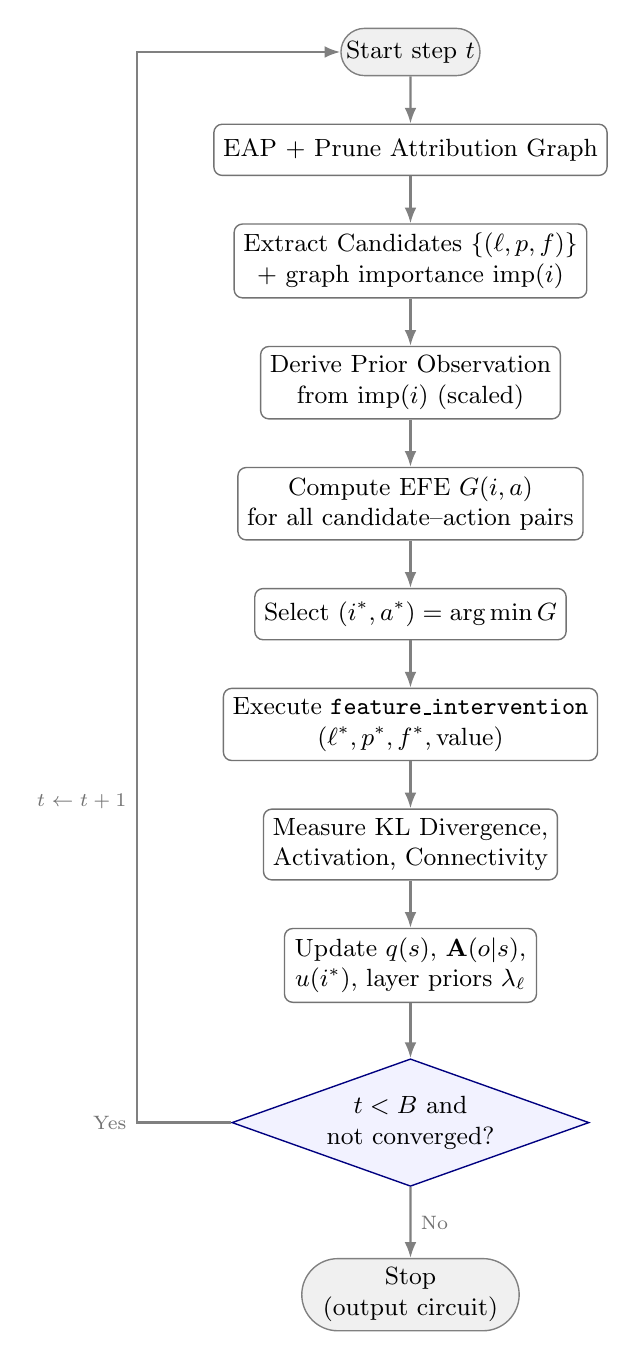
\begin{tikzpicture}[
    font=\small,
    node distance=0.6cm,
    flowstep/.style={
        rectangle, draw=black!55, fill=white,
        rounded corners=3pt, minimum width=3.2cm, minimum height=0.65cm,
        align=center, line width=0.5pt, font=\small
    },
    decision/.style={
        diamond, draw=blue!50!black, fill=blue!5,
        aspect=2.8, minimum width=1.0cm, align=center,
        inner sep=2pt, font=\small, line width=0.5pt
    },
    terminal/.style={
        rounded rectangle, draw=black!50, fill=black!6,
        minimum width=2.0cm, minimum height=0.6cm,
        align=center, line width=0.5pt, font=\small
    },
    arr/.style={-{Latex[length=2mm]}, thick, draw=black!50},
    ann/.style={font=\scriptsize, text=black!55},
]

\node[terminal] (start) {Start step $t$};

\node[flowstep, below=of start] (eap) {EAP + Prune Attribution Graph};

\node[flowstep, below=of eap] (cand) {Extract Candidates $\{(\ell, p, f)\}$\\+ graph importance $\mathrm{imp}(i)$};

\node[flowstep, below=of cand] (prior) {Derive Prior Observation\\from $\mathrm{imp}(i)$ (scaled)};

\node[flowstep, below=of prior] (efe) {Compute EFE $G(i,a)$\\for all candidate--action pairs};

\node[flowstep, below=of efe] (select) {Select $(i^*,a^*) = \arg\min G$};

\node[flowstep, below=of select] (interv) {Execute \texttt{feature\_intervention}\\$(\ell^*,p^*,f^*,\mathrm{value})$};

\node[flowstep, below=of interv] (measure) {Measure KL Divergence,\\Activation, Connectivity};

\node[flowstep, below=of measure] (update) {Update $q(s)$, $\mathbf{A}(o|s)$,\\$u(i^*)$, layer priors $\lambda_\ell$};

\node[decision, below=0.7cm of update] (check) {$t < B$ and\\not converged?};

\node[terminal, below=0.9cm of check] (stop) {Stop\\(output circuit)};

% Arrows
\draw[arr] (start) -- (eap);
\draw[arr] (eap) -- (cand);
\draw[arr] (cand) -- (prior);
\draw[arr] (prior) -- (efe);
\draw[arr] (efe) -- (select);
\draw[arr] (select) -- (interv);
\draw[arr] (interv) -- (measure);
\draw[arr] (measure) -- (update);
\draw[arr] (update) -- (check);
\draw[arr] (check) -- (stop) node[midway, right, ann]{No};

\draw[arr] (check.west) -- ++(-1.2,0) |- (start.west)
    node[pos=0.0, left, ann]{Yes}
    node[pos=0.15, left, ann]{$t \gets t+1$};

\end{tikzpicture}
%
}
\caption{\DIFaddFL{Flow of a single intervention step in Active Circuit Discovery.}}
\label{fig:flow}
\end{figure}

\DIFaddend The engine implements three manipulation types, each dispatched
via the \texttt{feature\_in\-ter\-ven\-tion} API according to the
action selected by the POMDP agent at each step:

\DIFdelbegin \textbf{\DIFdel{Ablation:}} %DIFAUXCMD
\DIFdel{Sets }\DIFdelend \DIFaddbegin \DIFadd{Ablation sets }\DIFaddend transcoder feature $(l, p, f)$ to zero:
\begin{equation}
  \label{eq:ablation}
  \text{logits}_{\text{abl}} = \text{feature\_intervention}(\text{prompt},
  [(l, p, f, 0)])
\end{equation}

\DIFdelbegin \textbf{\DIFdel{Activation Patching:}} %DIFAUXCMD
\DIFdel{Replaces }\DIFdelend \DIFaddbegin \DIFadd{Activation patching replaces the }\DIFaddend feature activation with a
mean-centred reference value $r$:
\begin{equation}
  \label{eq:patching}
  \text{logits}_{\text{patch}} = \text{feature\_intervention}(\text{prompt},
  [(l, p, f, r)])
\end{equation}

\DIFdelbegin \textbf{\DIFdel{Feature Steering:}} %DIFAUXCMD
\DIFdel{Scales activation by }\DIFdelend \DIFaddbegin \DIFadd{Feature steering scales the activation by a }\DIFaddend multiplier $m$:
\begin{equation}
  \label{eq:steering}
  \text{logits}_{\text{steer}} = \text{feature\_intervention}(\text{prompt},
  [(l, p, f, a_i \cdot m)])
\end{equation}

where $a_i$ is the clean activation value of feature $i$.

Effect is measured via KL divergence between the clean and intervened
output distributions:
\begin{equation}
  \label{eq:kl_intervention}
  \text{KL}_i = D_{\text{KL}}\!\left(
    \text{softmax}(\text{logits}_{\text{interv}})
    \;\|\;
    \text{softmax}(\text{logits}_{\text{clean}})
  \right)
\end{equation}

The \texttt{feature\_intervention} API correctly propagates the
intervention through the replacement model's transcoder structure,
ensuring that the measured effect reflects the true causal contribution
of the feature rather than a residual-stream approximation.


\DIFdelbegin %DIFDELCMD < \begin{figure}[H]
%DIFDELCMD < \centering
%DIFDELCMD < \resizebox{!}{0.82\textheight}{%
%DIFDELCMD < % figures/circuit_flow.tex -- Single Intervention Step Flowchart (journal-quality TikZ)
%DIFDELCMD < \begin{tikzpicture}[
%DIFDELCMD <     font=\small,
%DIFDELCMD <     node distance=0.6cm,
%DIFDELCMD <     flowstep/.style={
%DIFDELCMD <         rectangle, draw=black!55, fill=white,
%DIFDELCMD <         rounded corners=3pt, minimum width=3.2cm, minimum height=0.65cm,
%DIFDELCMD <         align=center, line width=0.5pt, font=\small
%DIFDELCMD <     },
%DIFDELCMD <     decision/.style={
%DIFDELCMD <         diamond, draw=blue!50!black, fill=blue!5,
%DIFDELCMD <         aspect=2.8, minimum width=1.0cm, align=center,
%DIFDELCMD <         inner sep=2pt, font=\small, line width=0.5pt
%DIFDELCMD <     },
%DIFDELCMD <     terminal/.style={
%DIFDELCMD <         rounded rectangle, draw=black!50, fill=black!6,
%DIFDELCMD <         minimum width=2.0cm, minimum height=0.6cm,
%DIFDELCMD <         align=center, line width=0.5pt, font=\small
%DIFDELCMD <     },
%DIFDELCMD <     arr/.style={-{Latex[length=2mm]}, thick, draw=black!50},
%DIFDELCMD <     ann/.style={font=\scriptsize, text=black!55},
%DIFDELCMD < ]
%DIFDELCMD < 

%DIFDELCMD < \node[terminal] (start) {Start step $t$};
%DIFDELCMD < 

%DIFDELCMD < \node[flowstep, below=of start] (eap) {EAP + Prune Attribution Graph};
%DIFDELCMD < 

%DIFDELCMD < \node[flowstep, below=of eap] (cand) {Extract Candidates $\{(\ell, p, f)\}$\\+ graph importance $\mathrm{imp}(i)$};
%DIFDELCMD < 

%DIFDELCMD < \node[flowstep, below=of cand] (prior) {Derive Prior Observation\\from $\mathrm{imp}(i)$ (scaled)};
%DIFDELCMD < 

%DIFDELCMD < \node[flowstep, below=of prior] (efe) {Compute EFE $G(i,a)$\\for all candidate--action pairs};
%DIFDELCMD < 

%DIFDELCMD < \node[flowstep, below=of efe] (select) {Select $(i^*,a^*) = \arg\min G$};
%DIFDELCMD < 

%DIFDELCMD < \node[flowstep, below=of select] (interv) {Execute \texttt{feature\_intervention}\\$(\ell^*,p^*,f^*,\mathrm{value})$};
%DIFDELCMD < 

%DIFDELCMD < \node[flowstep, below=of interv] (measure) {Measure KL Divergence,\\Activation, Connectivity};
%DIFDELCMD < 

%DIFDELCMD < \node[flowstep, below=of measure] (update) {Update $q(s)$, $\mathbf{A}(o|s)$,\\$u(i^*)$, layer priors $\lambda_\ell$};
%DIFDELCMD < 

%DIFDELCMD < \node[decision, below=0.7cm of update] (check) {$t < B$ and\\not converged?};
%DIFDELCMD < 

%DIFDELCMD < \node[terminal, below=0.9cm of check] (stop) {Stop\\(output circuit)};
%DIFDELCMD < 

%DIFDELCMD < % Arrows
%DIFDELCMD < \draw[arr] (start) -- (eap);
%DIFDELCMD < \draw[arr] (eap) -- (cand);
%DIFDELCMD < \draw[arr] (cand) -- (prior);
%DIFDELCMD < \draw[arr] (prior) -- (efe);
%DIFDELCMD < \draw[arr] (efe) -- (select);
%DIFDELCMD < \draw[arr] (select) -- (interv);
%DIFDELCMD < \draw[arr] (interv) -- (measure);
%DIFDELCMD < \draw[arr] (measure) -- (update);
%DIFDELCMD < \draw[arr] (update) -- (check);
%DIFDELCMD < \draw[arr] (check) -- (stop) node[midway, right, ann]{No};
%DIFDELCMD < 

%DIFDELCMD < \draw[arr] (check.west) -- ++(-1.2,0) |- (start.west)
%DIFDELCMD <     node[pos=0.0, left, ann]{Yes}
%DIFDELCMD <     node[pos=0.15, left, ann]{$t \gets t+1$};
%DIFDELCMD < 

%DIFDELCMD < \end{tikzpicture}
%DIFDELCMD < %
%DIFDELCMD < }
%DIFDELCMD < %%%
%DIFDELCMD < \caption{%
{%DIFAUXCMD
\DIFdelFL{Flow of a single intervention step in Active Circuit Discovery.}}
%DIFAUXCMD
%DIFDELCMD < \label{fig:flow}
%DIFDELCMD < \end{figure}
%DIFDELCMD < 

%DIFDELCMD < %%%
\DIFdelend % =================================================================
\section{Experimental Setup}
\label{sec:setup}
\subsection{Models and Hardware}

The framework is evaluated on two transformer architectures.
Gemma-2-2B~\cite{team2024gemma} has 26 layers, a 2304-dimensional
hidden size, and 8 attention heads; its transcoders are drawn from
GemmaScope (\texttt{mwhanna/gemma-scope-transcoders}).
Llama-3.2-1B~\cite{Dubey2024llama} has 16 layers, a 2048-dimensional
hidden size, and 32 heads with grouped-query attention; its
transcoders are from \texttt{mntss/transcoder-Llama-3.2-1B}.
Both models use the \texttt{circuit-tracer} library~\cite{Anthropic2025CT}
with the TransformerLens backend for attribution graph construction
and transcoder-level interventions.

Experiments run on an NVIDIA DGX Spark with GB10 GPU (128\,GB unified
memory, CUDA 12.8, aarch64).  Colab notebooks reproduce results on a
free T4 GPU.

\subsection{Benchmarks}

\subsubsection{IOI Circuit Recovery}

The Indirect Object Identification \DIFdelbegin \DIFdel{(IOI) }\DIFdelend task, introduced by
Wang et al.~\cite{Wang2022}, tests whether the agent can identify
features causally responsible for predicting the indirect object.
Five prompts of the form
``When [A] and [B] went to the store, [A] gave the bag to \_\_''
are used, where the correct prediction is [B].  For each prompt,
the KL divergence caused by ablating each candidate feature via the
\texttt{feature\_intervention} API is measured.

\subsubsection{Multi-step Reasoning}
\label{sec:multistep_benchmark}

The multi-step reasoning benchmark probes whether the discovery agent
can localise features that mediate compositional inference rather than
the single-hop associations that dominate IOI.  Three prompts are
used, each requiring the model to chain two or more intermediate facts
before producing the target token: a transitive ordering prompt
(``If Alice is taller than Bob, and Bob is taller than Carol, then
the tallest person is''), a factual-chain prompt
(``The capital of France is Paris.  Paris is in Europe.  The continent
containing Paris is''), and a syllogistic prompt
(``All dogs are animals.  Fido is a dog.  Therefore Fido is'').
Unlike IOI, where causally critical features are concentrated in a
small set of late-layer name-mover heads, compositional reasoning is
expected to recruit earlier and middle layers that bind entities and
propagate intermediate results through the residual stream.  This
shifts the effective search distribution away from the tail of the
attribution graph and stresses the agent's ability to allocate its
budget across layers rather than exploit a known late-layer prior.
For each prompt the KL divergence between the clean and intervened
next-token distributions is measured, using the same $B=20$ budget
and the same bandit, \DIFdelbegin \DIFdel{greedy, }\DIFdelend \DIFaddbegin \DIFadd{UCB, greedy, EAP, }\DIFaddend random, and oracle baselines as the
IOI benchmark so that \DIFaddbegin \DIFadd{bounded }\DIFaddend oracle efficiency is directly comparable
across tasks. \DIFaddbegin \DIFadd{This is also the benchmark used to evaluate the
finer-layer-bin variant (Section~\ref{sec:stats_protocol}).
}\DIFaddend 

\subsubsection{Feature Steering}

Five concept prompts (Golden Gate Bridge, Eiffel Tower, Mount Everest,
Great Wall of China, Statue of Liberty).
For each, the top 10 features by graph importance are identified and
their activations scaled \DIFdelbegin \DIFdel{at multipliers $m \in \{0, 2, 5, 10\}$. }\DIFdelend \DIFaddbegin \DIFadd{across a multiplier sweep
$m \in \{0, 1.5, 2, 3, 5, 10\}$. Because large multipliers can push
activations out of distribution, the protocol (a) includes smaller factors
(1.5, 2, 3) to characterise the dose-response curve, and (b) adds a
random-feature control: a matched set of randomly chosen
lower-importance features steered at the same multipliers. Causal
control is evidenced only to the extent that circuit-selected features shift
predictions more than this control. For every steered feature the top-five
next-token probabilities are recorded at each multiplier, so that
concept amplification at large factors can be distinguished from generic
distributional collapse. }\DIFaddend The KL divergence and whether the
model's top\DIFaddbegin \DIFadd{-1}\DIFaddend  prediction changes are measured \DIFaddbegin \DIFadd{for both sets}\DIFaddend .

\subsubsection{Multi-Domain Benchmark}

\DIFdelbegin \DIFdel{To provide broad coverage across cognitive domains, the framework is }\DIFdelend \DIFaddbegin \DIFadd{The framework is also }\DIFaddend evaluated
across five cognitive domains with two prompts each:
geography (e.g.\ ``The capital of France is''),
mathematics (e.g.\ ``The square root of 64 is''),
science (e.g.\ ``Water is made of hydrogen and''),
logic (syllogistic reasoning), and
history (e.g.\ ``The year World War II ended was'').
This allows cross-domain comparison of circuit structure and layer
distribution.

\subsection{Experimental Prompts}

All prompts used in the experiments are listed below.  These are
defined in the experiment runner script \DIFaddbegin \DIFadd{(}\texttt{\DIFadd{run\_real\_experiments.py}}\DIFadd{) }\DIFaddend and
correspond exactly to the prompts whose results appear in the JSON
outputs \DIFaddbegin \DIFadd{under }\texttt{\DIFadd{results/}}\DIFaddend .

\DIFdelbegin \textbf{\DIFdel{IOI Circuit Recovery (5 prompts):}}
%DIFAUXCMD
\DIFdelend \DIFaddbegin \DIFadd{The five IOI prompts are:
}\DIFaddend \begin{quote}
``When John and Mary went to the store, John gave the bag to''
``After Alice and Bob finished lunch, Alice handed the receipt to''
``While Sarah and Tom were at the park, Sarah threw the ball to''
``When Emma and David arrived at the office, Emma passed the keys to''
``As Lisa and Mike left the restaurant, Lisa returned the coat to''
\end{quote}

\DIFdelbegin \textbf{\DIFdel{Multi-step Reasoning (3 prompts):}}
%DIFAUXCMD
\DIFdelend \DIFaddbegin \DIFadd{The three multi-step reasoning prompts are:
}\DIFaddend \begin{quote}
``If Alice is taller than Bob, and Bob is taller than Carol, then the tallest person is''
``The capital of France is Paris. Paris is in Europe. The continent containing Paris is''
``All dogs are animals. Fido is a dog. Therefore Fido is''
\end{quote}

\DIFdelbegin \textbf{\DIFdel{Feature Steering (5 concept prompts):}}
%DIFAUXCMD
\DIFdelend \DIFaddbegin \DIFadd{The five feature-steering concept prompts are:
}\DIFaddend \begin{quote}
``The Golden Gate Bridge is''
``The Eiffel Tower is located in''
``Mount Everest is the tallest''
``The Great Wall of China was built''
``The Statue of Liberty stands in''
\end{quote}

\DIFdelbegin \textbf{\DIFdel{Multi-Domain Benchmark (10 prompts, 2 per domain):}}
%DIFAUXCMD
\DIFdelend \DIFaddbegin \DIFadd{The ten multi-domain prompts, two per domain, are grouped by domain below.
}\DIFaddend Geography prompts:
\begin{quote}
``The capital of France is''
``The Golden Gate Bridge connects San Francisco to''
\end{quote}

Mathematics prompts:
\begin{quote}
``The square root of 64 is''
``If 2 + 3 = 5 then 3 + 4 =''
\end{quote}

Science prompts:
\begin{quote}
``Water is made of hydrogen and''
``The speed of light is approximately''
\end{quote}

Logic prompts:
\begin{quote}
``All mammals are warm-blooded. A whale is a mammal. Therefore a whale is''
``All birds have wings. A penguin is a bird. Therefore a penguin has''
\end{quote}

History prompts:
\begin{quote}
``The year World War II ended was''
``The first person to walk on the moon was''
\end{quote}

\subsection{Baselines}

\DIFdelbegin \DIFdel{Four baselines are compared.
}\DIFdelend \DIFaddbegin \DIFadd{Baselines are grouped into ablation-only selectors (which, like POMDP-abl,
only ablate and are therefore directly comparable to the ablation oracle) and
action-matched selectors (which, like the full POMDP, may also steer, and
are used only for the secondary RCK analysis of Section~\ref{sec:results}).
}

\DIFadd{Among the ablation-only baselines, }\DIFaddend \emph{Random} selection draws features uniformly at random
(\DIFdelbegin \DIFdel{10 trials, results averaged), as in
Equation~\ref{eq:random}}\DIFdelend \DIFaddbegin \DIFadd{Equation~\ref{eq:random}; $N=10$ trials, averaged)}\DIFaddend :
\begin{equation}
  \label{eq:random}
  a_t \sim \text{Uniform}(\mathcal{F})
\end{equation}
\DIFdelbegin %DIFDELCMD < 

%DIFDELCMD < %%%
\DIFdelend \emph{Greedy} selection ranks features in descending order of graph
node influence (sum of absolute adjacency weights), per
Equation~\ref{eq:greedy}:
\begin{equation}
  \label{eq:greedy}
  i^* = \arg\max_i \text{imp}(i)
\end{equation}
where $\text{imp}(i)$ is the sum of absolute adjacency weights for node
$i$ (defined in Equation~\ref{eq:importance}).
\DIFdelbegin %DIFDELCMD < 

%DIFDELCMD < %%%
\DIFdelend \DIFaddbegin \emph{\DIFadd{EAP}} \DIFadd{ranking is a direct Edge-Attribution-Patching baseline: candidates are
ordered by the magnitude of their }\emph{\DIFadd{direct attribution to the logit nodes}} \DIFadd{of
the }\texttt{\DIFadd{circuit-tracer}} \DIFadd{graph, i.e.\ the feature's column summed over the logit
rows of the adjacency matrix, $\mathrm{eap}(i)=\sum_{t\in\mathcal{L}}|W_{t,i}|$
(normalised to $[0,1]$). This isolates the classic EAP ``direct effect on the
output'' signal, distinct from the total bidirectional connectivity used by Greedy,
and provides an established-method point of comparison.
}\DIFaddend The \emph{bandit}
selector combines graph importance with a decaying uncertainty bonus
and learned per-layer priors, providing a comparison point that
separates the contribution of Active Inference from simpler
uncertainty heuristics\DIFdelbegin \DIFdel{, as in Equation~\ref{eq:bandit}}\DIFdelend :
\begin{equation}
  \label{eq:bandit}
  S(i) = \text{imp}(i)\cdot\lambda_\ell + \omega_e \cdot u(i)
\end{equation}
where $u(i)$ is the uncertainty bonus (initialised to 1, decayed on
visit) and $\lambda_\ell$ is the per-layer prior updated from
observations. \DIFdelbegin %DIFDELCMD < 

%DIFDELCMD < %%%
\DIFdelend \DIFaddbegin \DIFadd{A }\emph{\DIFadd{plain UCB}} \DIFadd{baseline removes these engineered
priors and instead applies the textbook UCB1 rule over layers, using the
observed KL as reward; it isolates how much of the heuristic bandit's
performance comes from its hand-built importance and locality priors
rather than from upper-confidence exploration alone.
}\DIFaddend The \emph{oracle} selects features in descending order
of true KL divergence, an upper bound that requires all ablations in
advance\DIFdelbegin \DIFdel{(Equation~\ref{eq:oracle})}\DIFdelend :
\begin{equation}
  \label{eq:oracle}
  i^* = \arg\max_i \text{KL}_i^{\text{abl}}
\end{equation}

\DIFaddbegin \DIFadd{The action-matched baselines separate the contribution of the agent's selection
policy from that of the steering action. Steering-enabled counterparts of the
heuristics are evaluated that use the identical selection order but apply the
feature-steering intervention: }\emph{\DIFadd{Greedy+steer}}\DIFadd{, }\emph{\DIFadd{Bandit+steer}}\DIFadd{, and
}\emph{\DIFadd{Random+steer}}\DIFadd{. A }\emph{\DIFadd{Random-action}} \DIFadd{baseline that selects a feature uniformly
at random and chooses its intervention type uniformly at random is also included,
isolating the value of learned action selection. (Activation patching to the zero reference
coincides with ablation in this setup, so this control effectively samples between
ablation and steering.) The
corresponding }\emph{\DIFadd{multi-action oracle}} \DIFadd{ranks features by
$\max(\text{KL}^{\text{abl}}_i,\text{KL}^{\text{steer}}_i)$.
}

\DIFaddend All methods use the same \texttt{feature\_intervention} API and
KL divergence metric.  Budgets are fixed at $B=20$ interventions
per prompt.

\subsection{\DIFdelbegin \DIFdel{Evaluation }\DIFdelend Metrics}

\DIFdelbegin \DIFdel{Four metrics are reported.  }\DIFdelend \DIFaddbegin \DIFadd{Metrics of two kinds are reported, and they are kept
strictly separate because they live on different scales: a bounded efficiency for
ablation-only selectors and a relative amplification factor for steering-enabled
selectors.
}

\DIFaddend \emph{Mean KL per intervention} is the average KL divergence across selected
features\DIFdelbegin \DIFdel{, where }\DIFdelend \DIFaddbegin \DIFadd{; }\DIFaddend higher values indicate that the method finds more causally important
features. \emph{Cumulative KL} \DIFaddbegin \DIFadd{(CumKL) }\DIFaddend is the total information gained over the
budget\DIFdelbegin \DIFdel{,
compared against the oracle to compute }\emph{\DIFdel{oracle efficiency}}
%DIFAUXCMD
\DIFdel{(Equation~\ref{eq:oracle_eff}):
}\DIFdelend \DIFaddbegin \DIFadd{.
}

\emph{\DIFadd{(i) Bounded oracle efficiency.}} \DIFadd{For }\emph{\DIFadd{ablation-only}} \DIFadd{methods (POMDP-abl,
Random, Greedy, EAP, Bandit, UCB), every selector and the oracle draw from the same
quantity, ablation KL, so their ratio to the ablation oracle is bounded in
$[0,100]\%$ and is interpretable as an efficiency:
}\DIFaddend \begin{equation}
  \label{eq:oracle_eff}
  \eta = \DIFdelbegin \DIFdel{\frac{\text{CumKL}_{\text{agent}}}{\text{CumKL}_{\text{oracle}}} }\DIFdelend \DIFaddbegin \DIFadd{\frac{\text{CumKL}^{\text{abl}}_{\text{agent}}}{\text{CumKL}^{\text{abl}}_{\text{oracle}}} }\DIFaddend \times 100\%\DIFaddbegin \DIFadd{,
  \qquad \eta \in }[\DIFadd{0,100}]\DIFadd{\%.
}\DIFaddend \end{equation}
\DIFdelbegin \DIFdel{indicating how close a method is to optimal. }\DIFdelend \DIFaddbegin \DIFadd{This is the primary discovery-quality metric.
}

\emph{\DIFadd{(ii) Relative Cumulative KL (RCK).}} \DIFadd{The full multi-action agent may steer,
and steering can produce larger KL shifts than ablation; comparing its cumulative
KL to the }\emph{\DIFadd{ablation}} \DIFadd{oracle is therefore a ratio of two different quantities,
not a bounded efficiency, and can exceed $100\%$. This quantity is named the
Relative Cumulative KL,
}\begin{equation}
  \DIFadd{\label{eq:rck}
  \text{RCK} = \frac{\text{CumKL}_{\text{agent}}}{\text{CumKL}^{\text{abl}}_{\text{oracle}}} \times 100\%,
}\end{equation}
\DIFadd{and report it only for the action-matched analysis, explicitly labelled as a
relative amplification factor rather than an efficiency. All action-matched
baselines (Greedy+steer, Bandit+steer, Random+steer, Random-action) are reported on
the same RCK scale so the comparison is fair.
}\DIFaddend The KL divergence per intervention is computed as in Equation~\ref{eq:kl_def}:
\begin{equation}
  \label{eq:kl_def}
  D_\mathrm{KL}(p \,\|\, q) = \sum_t p(t)\log\frac{p(t)}{q(t)}
\end{equation}
The \emph{prediction change rate} is the fraction of steering experiments
in which the model's top-1 prediction changes.

\DIFdelbegin \DIFdel{The oracle
and all baselines use ablation-only KLdivergences, whereas the POMDP agent may select patching or steering interventions
whose KLmagnitudes differ from ablation. Oracle efficiency therefore
measures how well the agent identifies causally important features
relative to an }\DIFdelend \DIFaddbegin \DIFadd{In summary, the primary discovery-quality claim uses the bounded oracle
efficiency of Equation~\ref{eq:oracle_eff} applied to the }\DIFaddend ablation-only \DIFdelbegin \DIFdel{upper bound.
This is a
conservative
comparison: the agentis penalised for exploratory patching or
steering steps that may produce lower KL than ablation of the same
feature. The Correspondence Metric is
formally defined in Appendix~\ref{app:correspondence}}\DIFdelend \DIFaddbegin \DIFadd{agent
(POMDP-abl) against the ablation oracle, so that all quantities are on the same
scale and the metric cannot exceed $100\%$. The RCK of Equation~\ref{eq:rck} is
reported separately as a relative amplification factor for the full
multi-action agent and its action-matched baselines, never as an efficiency.
The Correspondence Metric is formally defined in Appendix~\ref{app:correspondence}.
}

\subsection{\DIFadd{Statistical Analysis and Sensitivity}}
\label{sec:stats_protocol}

\DIFadd{Given the modest prompt counts and the
high coefficient of variation of per-prompt KL, every reported mean,
bounded efficiency, and RCK is accompanied by a percentile bootstrap 95\% confidence
interval obtained by resampling prompts with replacement ($10^4$ resamples).
Hypothesis H1 is assessed by both a one-sided paired $t$-test and an exact
paired-permutation test of agent-versus-random per-prompt mean KL; a result is
reported as significant only when $p<0.05$ under the permutation test. H1 is not
accepted where it is not significant (for example, Llama IOI).
}

\DIFadd{The discretisation sensitivity of the agent is assessed at $\pm 20\%$. The agent discretises
continuous observations (KL, activation, connectivity) at fixed thresholds, and maps
graph importance into the KL-prior range through a $0.01$ scaling factor
(Appendix~\ref{app:generative_model}). To show that conclusions are not artefacts of
these choices, the Gemma IOI benchmark is re-run with the KL and activation
thresholds independently scaled by $0.8$ and $1.2$, and the resulting change in
bounded efficiency is reported. The scaling is exposed through the experiment runner
flags }\texttt{\DIFadd{-}{}\DIFadd{-kl-threshold-scale}}\DIFadd{, }\texttt{\DIFadd{-}{}\DIFadd{-act-threshold-scale}}\DIFadd{, and
}\texttt{\DIFadd{-}{}\DIFadd{-imp-scale}}\DIFaddend .

\DIFaddbegin \DIFadd{To characterise robustness to the agent's
core hyperparameters, the Gemma and Llama IOI benchmarks are additionally re-run
while independently varying the action precision ($\gamma \in \{4, 16, 64\}$), the
Dirichlet likelihood learning rate ($\eta \in \{0.5, 1.0, 2.0\}$), and the pragmatic
preference weight ($\{0.5, 1.0, 2.0\}$), one factor at a time about the default.
These factors are exposed through }\texttt{\DIFadd{-}{}\DIFadd{-gamma}}\DIFadd{, }\texttt{\DIFadd{-}{}\DIFadd{-lr-pa}}\DIFadd{, and
}\texttt{\DIFadd{-}{}\DIFadd{-pragmatic-weight}}\DIFadd{, and the resulting bounded efficiencies are reported in
Section~\ref{sec:results}.
}

\DIFadd{To probe the Llama multi-step result, a
variant is additionally run in which the agent's single layer-role factor is
refined from 3 bins (early/middle/late) to 6, via }\texttt{\DIFadd{-}{}\DIFadd{-n-layer-role 6}}\DIFadd{, so
that deeper layer structure can be represented in the belief state. The outcome is
reported in Section~\ref{sec:results} regardless of whether it improves the result.
}

\DIFaddend \subsection{POMDP Agent Configuration}

The Active Inference POMDP agent \DIFdelbegin \DIFdel{operates across }\DIFdelend \DIFaddbegin \DIFadd{uses 4 importance levels $\times$
3 layer roles $\times$ 3 causal influence levels for a total of }\DIFaddend 36
\DIFdelbegin \DIFdel{joint hidden states, derived from a combination of four importance levels , three layer roles , and three levels of causal influence }\DIFdelend \DIFaddbegin \DIFadd{joint hidden states}\DIFaddend .  Observations comprise 4 KL levels, 4 activation
levels, and 3 connectivity levels.  The agent selects among 3 actions
(ablation, patching, steering) using a single-step lookahead policy
with stochastic selection via softmax over negative EFE
($\gamma = 16.0$).  The observation model is learned online through
Dirichlet updates on all modalities ($\eta = 1.0$), and inference
uses the vanilla variational scheme implemented in pymdp.

\subsection{Reproducibility}

All code is available at
\url{https://github.com/SharathSPhD/ActiveCIrcuitDiscovery}.
Colab notebooks reproduce the main experiments on a free T4 GPU.
The experiment runner supports model selection via
\texttt{-{}-model gemma|llama|both} and benchmark selection via
\texttt{-{}-experiment ioi|steering|multistep|domain|all}.
Raw experiment outputs are stored in \texttt{results/} as JSON.

The \ACD{} framework \DIFdelbegin \DIFdel{is packaged as a Docker container targeting }\DIFdelend \DIFaddbegin \DIFadd{ships with two Docker targets so that results are not
tied to a single architecture.  }\texttt{\DIFadd{Dockerfile.dgx-spark}} \DIFadd{(with
}\texttt{\DIFadd{docker-compose.yml}}\DIFadd{) targets }\DIFaddend the NVIDIA DGX Spark platform \DIFaddbegin \DIFadd{on which
the headline numbers were produced }\DIFaddend (GB10 GPU, 128~GB unified memory,
CUDA~12.8, aarch64\DIFdelbegin \DIFdel{architecture).  The }\DIFdelend \DIFaddbegin \DIFadd{).  }\DIFaddend \texttt{\DIFdelbegin \DIFdel{docker-compose}\DIFdelend \DIFaddbegin \DIFadd{Dockerfile}\DIFaddend .\DIFdelbegin \DIFdel{yml}\DIFdelend \DIFaddbegin \DIFadd{amd64}\DIFaddend } \DIFdelbegin \DIFdel{in the repository
root provides volume mounts for model weights (cached from HuggingFace Hub)
and result directories.  The container installs }\DIFdelend \DIFaddbegin \DIFadd{(with
}\texttt{\DIFadd{docker-compose.amd64.yml}}\DIFadd{) provides a standard }\texttt{\DIFadd{x86\_64}}
\DIFadd{image built on the upstream }\texttt{\DIFadd{pytorch/pytorch:2.4.0-cuda12.1}} \DIFadd{base; it
runs on any NVIDIA GPU of compute capability $\geq 7.5$, including the
16~GB T4 offered for free on Google Colab.  Because the model loads in
float32 and uses only $\sim$5~GB of VRAM, the full pipeline fits on a single
T4, and the accompanying Colab notebooks reproduce the IOI, steering,
multi-step, and domain experiments end-to-end on that hardware.  Both images
install }\DIFaddend \texttt{circuit-tracer} from source and \DIFdelbegin \DIFdel{pins all }\DIFdelend \DIFaddbegin \DIFadd{pin all remaining
}\DIFaddend dependencies via \texttt{requirements.txt}\DIFaddbegin \DIFadd{; absolute KL values can shift
marginally across GPU generations and driver/cuDNN versions, but the
relative orderings and statistical conclusions reported here are
hardware-independent}\DIFaddend .

Gemma-2-2B is available from HuggingFace Hub under the Gemma license
(\texttt{google/\allowbreak gemma-2-2b}),
and GemmaScope transcoders are fetched automatically by the \texttt{circuit-tracer} library.
Experiments require a single NVIDIA GPU with at least 8~GB VRAM (tested on T4 with 16~GB in Colab
and GB10 with 128~GB on DGX Spark). The model loads in float32 and requires approximately 5~GB VRAM.
All dependencies are pinned in \texttt{requirements.txt}, with key packages including \texttt{circuit-tracer}
(from git), \texttt{transformer-lens}, and \texttt{torch>=2.0}.

Random baselines use \texttt{numpy.random.seed(42)}, while the Active Inference Selector is
deterministic given the same candidates and exploration weight.
Approximate runtime is 40--60 seconds per prompt on a single GPU (attribution graph generation: $\sim$18s;
40 ablations at $\sim$30ms each: $\sim$1.2s; overhead: $\sim$20s for model setup on first prompt).
All experiment outputs are saved as JSON in the \texttt{results/} directory, including per-prompt KL values
for all methods, feature IDs, layer distributions, and steering outcomes.


% =================================================================
\section{Results}
\label{sec:results}
% Results populated from real experiment runs on Gemma-2-2B and Llama-3.2-1B.
%DIF <  Experiments executed on NVIDIA GB10 (DGX Spark), Feb 2026.
%DIF >  Experiments executed on NVIDIA GB10 (DGX Spark), May 2026.
% True online multi-action POMDP with action-conditioned B-matrix.
%DIF >  All numbers traceable to results/*.json via scripts/compute_paper_stats.py.

\subsection{IOI Circuit Recovery}

\DIFdelbegin \DIFdel{Circuit discovery }\DIFdelend \DIFaddbegin \DIFadd{Intervention-selection quality is first evaluated }\DIFaddend on the Indirect Object
Identification (IOI) task\DIFdelbegin \DIFdel{is
evaluated using }\DIFdelend \DIFaddbegin \DIFadd{: }\DIFaddend 5 prompts with a budget of \DIFdelbegin \DIFdel{20 }\DIFdelend \DIFaddbegin \DIFadd{$B=20$
}\DIFaddend feature-level interventions per prompt.  The \DIFdelbegin \DIFdel{POMDP agent selects both the
target feature and the
intervention type (ablation , activation patching, or feature steering) at
each step via EFE minimisation.  Baselines use ablation-only KL divergences (see }\DIFdelend \DIFaddbegin \DIFadd{fair comparison fixes the
intervention type to ablation for every method, so that all
strategies are scored on the same ablation-KL scale against an
ablation oracle that greedily ranks the candidate set by true ablation
KL (}\DIFaddend Section~\ref{sec:setup}).  \DIFdelbegin \DIFdel{Aggregate discovery
performance across both models is summarised in
}\DIFdelend \DIFaddbegin \DIFadd{Under this protocol the agent is the
ablation-constrained variant }\emph{\DIFadd{POMDP-abl}}\DIFadd{, which uses the full
Expected Free Energy (EFE) objective to choose which feature to
test but is denied the steering action.  The multi-action agent that
also chooses the intervention type is analysed separately in
Section~\ref{sec:rck}.  Mean and median per-step KL and the
bounded oracle efficiency (cumulative method KL divided by
cumulative oracle KL, $\leq 100\%$ by construction) are reported with bootstrap
95\% confidence intervals over prompts (}\DIFaddend Table~\ref{tab:ioi}\DIFaddbegin \DIFadd{)}\DIFaddend .

\begin{table}[H]
\centering
\caption{IOI \DIFdelbeginFL \DIFdelFL{Feature Discovery}\DIFdelendFL \DIFaddbeginFL \DIFaddFL{feature discovery under the fair ablation-only protocol}\DIFaddendFL :
\DIFdelbeginFL \DIFdelFL{Mean }\DIFdelendFL \DIFaddbeginFL \DIFaddFL{per-prompt mean }\DIFaddendFL KL\DIFdelbeginFL \DIFdelFL{($\pm$ std) per Intervention}\DIFdelendFL \DIFaddbeginFL \DIFaddFL{, median, inter-quartile range }[\DIFaddFL{Q1, Q3}]\DIFaddFL{, and bounded
oracle efficiency with bootstrap 95\% CIs over 5 prompts.}\DIFaddendFL }
\label{tab:ioi}
{\small
\DIFdelbeginFL %DIFDELCMD < \begin{tabular}{llccc}
%DIFDELCMD < %%%
\DIFdelendFL \DIFaddbeginFL \begin{tabular}{llcccc}
\DIFaddendFL \toprule
\textbf{Model} & \textbf{Method} & \textbf{Mean KL} & \textbf{\DIFdelbeginFL \DIFdelFL{$\pm$ std}\DIFdelendFL \DIFaddbeginFL \DIFaddFL{Median}\DIFaddendFL } & \textbf{\DIFdelbeginFL \DIFdelFL{Oracle Eff.}\DIFdelendFL \DIFaddbeginFL [\DIFaddFL{Q1, Q3}]\DIFaddendFL } \DIFaddbeginFL & \textbf{\DIFaddFL{Oracle Eff.\ [95\% CI]}} \DIFaddendFL \\
\midrule
\DIFdelbeginFL %DIFDELCMD < \multirow{5}{*}{Gemma-2-2B}
%DIFDELCMD <  %%%
\DIFdelendFL \DIFaddbeginFL \multirow{7}{*}{Gemma-2-2B}
 \DIFaddendFL & \DIFdelbeginFL \DIFdelFL{POMDP Agent }\DIFdelendFL \DIFaddbeginFL \DIFaddFL{Oracle      }\DIFaddendFL & \DIFdelbeginFL \textbf{\DIFdelFL{0.010824}} %DIFAUXCMD
\DIFdelendFL \DIFaddbeginFL \DIFaddFL{0.000862 }\DIFaddendFL & \DIFdelbeginFL \DIFdelFL{0.005700 }\DIFdelendFL \DIFaddbeginFL \DIFaddFL{---      }\DIFaddendFL & \DIFdelbeginFL \textbf{\DIFdelFL{1255.0\%}} %DIFAUXCMD
\DIFdelendFL \DIFaddbeginFL \DIFaddFL{---                    }& \DIFaddFL{100.0\% }\DIFaddendFL \\
 & \DIFdelbeginFL \DIFdelFL{Oracle      }\DIFdelendFL \DIFaddbeginFL \DIFaddFL{EAP         }\DIFaddendFL & \DIFdelbeginFL \DIFdelFL{---      }\DIFdelendFL \DIFaddbeginFL \DIFaddFL{0.000793 }\DIFaddendFL & \DIFdelbeginFL \DIFdelFL{---      }\DIFdelendFL \DIFaddbeginFL \DIFaddFL{0.000436 }\DIFaddendFL & \DIFdelbeginFL \DIFdelFL{100.0\% }\DIFdelendFL \DIFaddbeginFL [\DIFaddFL{0.000399, 0.001306}]   & \DIFaddFL{91.9\% }[\DIFaddFL{82.1, 96.5}] \DIFaddendFL \\
 & \DIFaddbeginFL \DIFaddFL{POMDP-abl   }& \DIFaddFL{0.000707 }& \DIFaddFL{0.000404 }& [\DIFaddFL{0.000335, 0.001115}]   & \DIFaddFL{82.0\% }[\DIFaddFL{73.8, 87.8}] \\
 & \DIFaddendFL Bandit      & 0.000642 & \DIFdelbeginFL \DIFdelFL{0.000422 }\DIFdelendFL \DIFaddbeginFL \DIFaddFL{0.000408 }\DIFaddendFL & \DIFaddbeginFL [\DIFaddFL{0.000294, 0.001145}]   & \DIFaddendFL 74.4\% \DIFaddbeginFL [\DIFaddFL{67.9, 79.0}] \DIFaddendFL \\
 & \DIFaddbeginFL \DIFaddFL{UCB         }& \DIFaddFL{0.000635 }& \DIFaddFL{0.000394 }& [\DIFaddFL{0.000242, 0.001155}]   & \DIFaddFL{73.7\% }[\DIFaddFL{59.0, 82.2}] \\
 & \DIFaddendFL Greedy      & 0.000577 & \DIFdelbeginFL \DIFdelFL{0.000385 }\DIFdelendFL \DIFaddbeginFL \DIFaddFL{0.000492 }\DIFaddendFL & \DIFaddbeginFL [\DIFaddFL{0.000260, 0.000583}]   & \DIFaddendFL 66.9\% \DIFaddbeginFL [\DIFaddFL{47.5, 83.0}] \DIFaddendFL \\
 & Random      & \DIFdelbeginFL \DIFdelFL{0.000444 }\DIFdelendFL \DIFaddbeginFL \DIFaddFL{0.000493 }\DIFaddendFL & \DIFdelbeginFL \DIFdelFL{0.000272 }\DIFdelendFL \DIFaddbeginFL \DIFaddFL{0.000289 }\DIFaddendFL & \DIFdelbeginFL \DIFdelFL{51.5\% }\DIFdelendFL \DIFaddbeginFL [\DIFaddFL{0.000202, 0.000867}]   & \DIFaddFL{57.1\% }[\DIFaddFL{49.0, 60.2}] \DIFaddendFL \\
\midrule
\DIFdelbeginFL %DIFDELCMD < \multirow{5}{*}{Llama-3.2-1B}
%DIFDELCMD <  %%%
\DIFdelendFL \DIFaddbeginFL \multirow{7}{*}{Llama-3.2-1B}
 \DIFaddendFL & Oracle      & \DIFaddbeginFL \DIFaddFL{0.009755 }& \DIFaddendFL ---      & ---                    & 100.0\% \\
 & \DIFdelbeginFL \DIFdelFL{POMDP Agent }\DIFdelendFL \DIFaddbeginFL \DIFaddFL{EAP         }\DIFaddendFL & \DIFdelbeginFL \textbf{\DIFdelFL{0.008833}} %DIFAUXCMD
\DIFdelendFL \DIFaddbeginFL \DIFaddFL{0.009291 }\DIFaddendFL & \DIFdelbeginFL \DIFdelFL{0.006900 }\DIFdelendFL \DIFaddbeginFL \DIFaddFL{0.005739 }\DIFaddendFL & \DIFdelbeginFL \textbf{\DIFdelFL{90.6\%}}  %DIFAUXCMD
\DIFdelendFL \DIFaddbeginFL [\DIFaddFL{0.003297, 0.018357}]   & \DIFaddFL{95.2\% }[\DIFaddFL{87.0, 97.7}] \DIFaddendFL \\
 & Bandit      & 0.008606 & \DIFdelbeginFL \DIFdelFL{0.006910 }\DIFdelendFL \DIFaddbeginFL \DIFaddFL{0.005999 }\DIFaddendFL & \DIFaddbeginFL [\DIFaddFL{0.003302, 0.014895}]   & \DIFaddendFL 88.2\% \DIFaddbeginFL [\DIFaddFL{79.0, 96.7}] \DIFaddendFL \\
 & \DIFaddbeginFL \DIFaddFL{UCB         }& \DIFaddFL{0.005389 }& \DIFaddFL{0.001458 }& [\DIFaddFL{0.001227, 0.006000}]   & \DIFaddFL{55.2\% }[\DIFaddFL{10.5, 92.7}] \\
 & \DIFaddFL{POMDP-abl   }& \DIFaddFL{0.005086 }& \DIFaddFL{0.002679 }& [\DIFaddFL{0.001923, 0.006294}]   & \DIFaddFL{52.1\% }[\DIFaddFL{17.4, 90.2}] \\
 & \DIFaddendFL Random      & \DIFdelbeginFL \DIFdelFL{0.003622 }\DIFdelendFL \DIFaddbeginFL \DIFaddFL{0.004720 }\DIFaddendFL & \DIFdelbeginFL \DIFdelFL{0.002866 }\DIFdelendFL \DIFaddbeginFL \DIFaddFL{0.001795 }\DIFaddendFL & \DIFdelbeginFL \DIFdelFL{37.1\% }\DIFdelendFL \DIFaddbeginFL [\DIFaddFL{0.001504, 0.007315}]   & \DIFaddFL{48.4\% }[\DIFaddFL{31.6, 64.7}] \DIFaddendFL \\
 & Greedy      & 0.003982 & \DIFdelbeginFL \DIFdelFL{0.005053 }\DIFdelendFL \DIFaddbeginFL \DIFaddFL{0.001923 }\DIFaddendFL & \DIFaddbeginFL [\DIFaddFL{0.000899, 0.002689}]   & \DIFaddendFL 40.8\% \DIFaddbeginFL [\DIFaddFL{11.7, 74.1}] \DIFaddendFL \\
\bottomrule
\end{tabular}
}
\end{table}

\DIFdelbegin \DIFdel{Results are averaged over 5 IOI prompts with $B=20$ interventions.
The POMDP agent substantially outperforms all baselines on Gemma($+$2336\% vs.
\ random, oracle efficiency 1255}\DIFdelend \DIFaddbegin \DIFadd{The efficiency denominator is the oracle's per-step mean KL, $0.000862$
(Gemma) and $0.009755$ (Llama), equivalently a cumulative KL of $0.0172$
(Gemma) and $0.1951$ (Llama) over the 20-step budget.
On Gemma, POMDP-abl reaches 82.0\% of the ablation oracle, clearly
above random (57.1}\DIFaddend \%) and \DIFdelbegin \DIFdel{outperforms
all baselines on Llama (oracle efficiency 90.6\%) .  Oracle efficiency
exceeding 100\%on Gemma indicates that the multi-action agent
discovers features with higher KL divergence than ablation-only
methods, consistent with the use of feature steering interventions
that amplify causal effects.  This arises because the
oracle baseline
uses only ablation-based KL divergences, whereas the POMDP agentcan
select feature steering interventions that amplify causal effects
beyond the
baseline effects observed under ablation.  When a feature
carries multiplicative causal influence, steering (which scales the
feature activation)can produce higher KL divergence than ablation on
the same feature---a genuine capability rather than a measurement
artefact}\DIFdelend \DIFaddbegin \DIFadd{greedy (66.9\%) and modestly above the
heuristic bandit (74.4\%) and the plain UCB baseline (73.7\%).  A
one-sided paired permutation test confirms the
gain over random ($+43.5\%$ relative, $p=0.031$, $n=5$).  A
direct EAP attribution ranking is itself a strong ablation-KL baseline
(91.9\%) and is not surpassed by the agent.  On Llama the
picture is less favourable: POMDP-abl (52.1\%) only matches random
(48.4\%) and the plain UCB baseline (55.2\%), and trails both the
heuristic bandit (88.2\%) and EAP (95.2\%); the
gain over random is small and not significant ($+7.8\%$, $p=0.41$).
No efficiency win is therefore claimed over the strongest
ablation baselines, since EAP ranking is competitive or better in every
tested setting; the agent's contribution is instead positioned as
an adaptive, uncertainty-aware intervention-selection policy
(Sections~\ref{sec:rck} and~\ref{sec:discussion})}\DIFaddend .

The temporal profile \DIFdelbegin \DIFdel{of this advantage }\DIFdelend \DIFaddbegin \DIFadd{under the fair protocol }\DIFaddend is shown in
Figure~\ref{fig:cumkl}\DIFdelbegin \DIFdel{on Gemma the POMDP agent's cumulative KL curve
dominates all
baselines from roughly step four onward and tracks }\DIFdelend \DIFaddbegin \DIFadd{.  The cumulative ablation-KL curves of all
ablation-only methods are plotted against }\DIFaddend the oracle envelope\DIFaddbegin \DIFadd{: on
Gemma, EAP tracks the oracle most closely, with POMDP-abl, bandit and
greedy bunched below it}\DIFaddend ; on Llama \DIFdelbegin \DIFdel{it remains competitive with }\DIFdelend the bandit and \DIFdelbegin \DIFdel{clearly above random and greedy throughout the 20-step budget}\DIFdelend \DIFaddbegin \DIFadd{EAP lead while
POMDP-abl tracks greedy and random.  No method exceeds the oracle, as
expected when all methods share the ablation action}\DIFaddend .

\begin{figure}[H]
\centering
% Auto-generated from experiment results.
\DIFdelbeginFL %DIFDELCMD < \begin{tikzpicture}
%DIFDELCMD < \begin{groupplot}[
%DIFDELCMD <     group style={
%DIFDELCMD <         group size=2 by 1,
%DIFDELCMD <         horizontal sep=0.5cm,
%DIFDELCMD <         ylabels at=edge left,
%DIFDELCMD <     },
%DIFDELCMD <     width=0.48\linewidth,
%DIFDELCMD <     height=6cm,
%DIFDELCMD <     x label style={font=\scriptsize},
%DIFDELCMD <     y label style={font=\scriptsize},
%DIFDELCMD <     tick label style={font=\scriptsize},
%DIFDELCMD <     title style={font=\scriptsize\bfseries},
%DIFDELCMD <     legend style={
%DIFDELCMD <         font=\tiny,
%DIFDELCMD <         at={(0.5,-0.30)},
%DIFDELCMD <         anchor=north,
%DIFDELCMD <         legend columns=4,
%DIFDELCMD <         /tikz/every even column/.append style={column sep=0.3cm}
%DIFDELCMD <     },
%DIFDELCMD <     ymajorgrids=true,
%DIFDELCMD <     grid style={dashed, gray!30},
%DIFDELCMD < ]
%DIFDELCMD < 

%DIFDELCMD < \nextgroupplot[title={Gemma-2-2B},
%DIFDELCMD <     xlabel={Intervention step},
%DIFDELCMD <     ylabel={Cumulative KL},
%DIFDELCMD <     xmin=1, xmax=20,
%DIFDELCMD < ]
%DIFDELCMD < 

%DIFDELCMD < \addplot[black, dashed, thick] coordinates { (1,0.007569) (2,0.010324) (3,0.012028) (4,0.013152) (5,0.013773) (6,0.014261) (7,0.014671) (8,0.015055) (9,0.015355) (10,0.015627) (11,0.015880) (12,0.016120) (13,0.016327) (14,0.016520) (15,0.016703) (16,0.016861) (17,0.016978) (18,0.017086) (19,0.017175) (20,0.017249) };
%DIFDELCMD < \addplot[red, thick] coordinates { (1,0.000361) (2,0.011055) (3,0.011487) (4,0.060636) (5,0.061124) (6,0.062139) (7,0.062873) (8,0.100012) (9,0.113948) (10,0.117111) (11,0.143585) (12,0.191522) (13,0.197228) (14,0.199761) (15,0.200720) (16,0.203605) (17,0.207116) (18,0.215377) (19,0.215929) (20,0.216471) };
%DIFDELCMD < \addplot[orange, thick] coordinates { (1,0.000361) (2,0.000573) (3,0.004776) (4,0.005562) (5,0.006226) (6,0.006944) (7,0.007926) (8,0.008343) (9,0.008482) (10,0.008796) (11,0.008850) (12,0.008900) (13,0.009708) (14,0.012222) (15,0.012265) (16,0.012462) (17,0.012526) (18,0.012568) (19,0.012748) (20,0.012840) };
%DIFDELCMD < \addplot[blue, thick] coordinates { (1,0.000361) (2,0.000692) (3,0.001201) (4,0.005808) (5,0.006035) (6,0.006726) (7,0.006917) (8,0.007597) (9,0.007841) (10,0.008781) (11,0.008886) (12,0.009513) (13,0.009535) (14,0.009680) (15,0.009864) (16,0.009893) (17,0.009943) (18,0.010027) (19,0.010054) (20,0.011541) };
%DIFDELCMD < 

%DIFDELCMD < \legend{Oracle, POMDP Agent, Bandit, Greedy}
%DIFDELCMD < 

%DIFDELCMD < \nextgroupplot[title={Llama-3.2-1B},
%DIFDELCMD <     xlabel={Intervention step},
%DIFDELCMD <     ylabel={Cumulative KL},
%DIFDELCMD <     xmin=1, xmax=20,
%DIFDELCMD < ]
%DIFDELCMD < 

%DIFDELCMD < \addplot[black, dashed, thick] coordinates { (1,0.150922) (2,0.174142) (3,0.182066) (4,0.185418) (5,0.187425) (6,0.189116) (7,0.190533) (8,0.191621) (9,0.192344) (10,0.192876) (11,0.193291) (12,0.193617) (13,0.193901) (14,0.194161) (15,0.194402) (16,0.194627) (17,0.194784) (18,0.194906) (19,0.195004) (20,0.195095) };
%DIFDELCMD < \addplot[red, thick] coordinates { (1,0.002216) (2,0.003179) (3,0.003793) (4,0.004274) (5,0.006622) (6,0.008522) (7,0.010877) (8,0.013939) (9,0.075828) (10,0.077331) (11,0.078285) (12,0.143502) (13,0.146003) (14,0.146062) (15,0.146401) (16,0.147294) (17,0.149689) (18,0.175889) (19,0.176116) (20,0.176665) };
%DIFDELCMD < \addplot[orange, thick] coordinates { (1,0.000635) (2,0.002159) (3,0.003260) (4,0.056815) (5,0.056850) (6,0.070795) (7,0.070796) (8,0.070840) (9,0.070988) (10,0.091854) (11,0.092100) (12,0.095000) (13,0.099887) (14,0.100413) (15,0.100669) (16,0.101838) (17,0.102465) (18,0.171571) (19,0.171662) (20,0.172120) };
%DIFDELCMD < \addplot[blue, thick] coordinates { (1,0.000635) (2,0.002851) (3,0.003814) (4,0.004144) (5,0.004313) (6,0.004715) (7,0.005854) (8,0.006438) (9,0.007958) (10,0.008415) (11,0.062141) (12,0.062909) (13,0.063706) (14,0.072875) (15,0.072998) (16,0.073181) (17,0.073229) (18,0.074028) (19,0.079534) (20,0.079641) };
%DIFDELCMD < 

%DIFDELCMD < \end{groupplot}
%DIFDELCMD < \end{tikzpicture}
%DIFDELCMD < %%%
\DIFdelendFL \DIFaddbeginFL 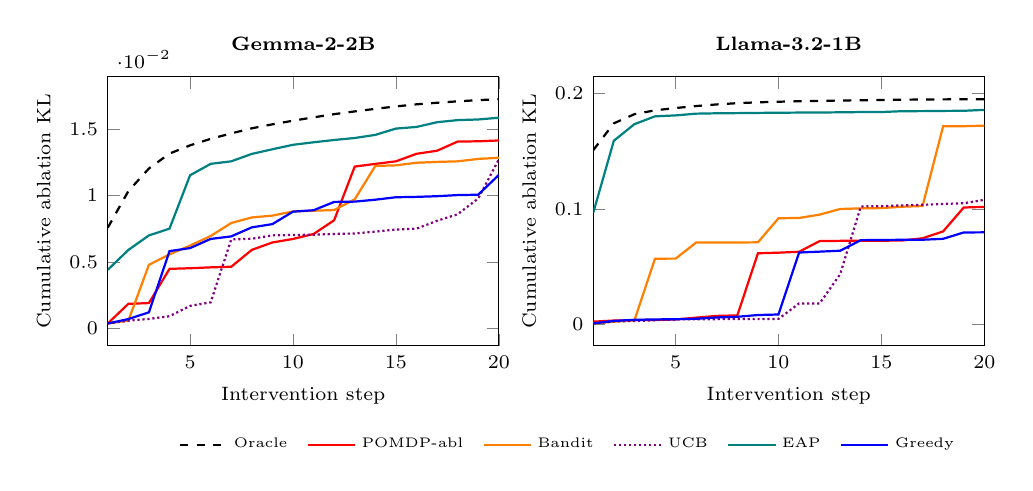
\begin{tikzpicture}
\begin{groupplot}[
    group style={
        group size=2 by 1,
        horizontal sep=1.2cm,
        ylabels at=edge left,
    },
    width=0.54\columnwidth,
    height=5.0cm,
    x label style={font=\scriptsize},
    y label style={font=\scriptsize},
    tick label style={font=\scriptsize},
    title style={font=\scriptsize\bfseries},
    legend style={
        font=\tiny, legend columns=-1, draw=none,
        at={(1.18,-0.30)}, anchor=north,
        /tikz/every even column/.append style={column sep=5pt},
    },
]

\nextgroupplot[title={Gemma-2-2B},
    xlabel={Intervention step},
    ylabel={Cumulative ablation KL},
    xmin=1, xmax=20,
]

\addplot[black, dashed, thick] coordinates { (1,0.007569) (2,0.010324) (3,0.012028) (4,0.013152) (5,0.013773) (6,0.014261) (7,0.014671) (8,0.015055) (9,0.015355) (10,0.015627) (11,0.015880) (12,0.016120) (13,0.016327) (14,0.016520) (15,0.016703) (16,0.016861) (17,0.016978) (18,0.017086) (19,0.017175) (20,0.017249) };
\addplot[red, thick] coordinates { (1,0.000361) (2,0.001838) (3,0.001897) (4,0.004472) (5,0.004520) (6,0.004586) (7,0.004632) (8,0.005904) (9,0.006459) (10,0.006726) (11,0.007096) (12,0.008134) (13,0.012175) (14,0.012376) (15,0.012568) (16,0.013134) (17,0.013366) (18,0.014055) (19,0.014077) (20,0.014140) };
\addplot[orange, thick] coordinates { (1,0.000361) (2,0.000573) (3,0.004776) (4,0.005562) (5,0.006226) (6,0.006944) (7,0.007926) (8,0.008343) (9,0.008482) (10,0.008796) (11,0.008850) (12,0.008900) (13,0.009708) (14,0.012222) (15,0.012265) (16,0.012462) (17,0.012526) (18,0.012568) (19,0.012748) (20,0.012840) };
\addplot[violet, thick, densely dotted] coordinates { (1,0.000361) (2,0.000571) (3,0.000703) (4,0.000906) (5,0.001685) (6,0.001951) (7,0.006689) (8,0.006738) (9,0.006993) (10,0.007022) (11,0.007042) (12,0.007101) (13,0.007137) (14,0.007277) (15,0.007431) (16,0.007496) (17,0.008092) (18,0.008583) (19,0.009771) (20,0.012705) };
\addplot[teal, thick] coordinates { (1,0.004399) (2,0.005895) (3,0.006990) (4,0.007500) (5,0.011519) (6,0.012379) (7,0.012569) (8,0.013128) (9,0.013477) (10,0.013813) (11,0.014002) (12,0.014175) (13,0.014325) (14,0.014559) (15,0.015033) (16,0.015157) (17,0.015514) (18,0.015671) (19,0.015720) (20,0.015851) };
\addplot[blue, thick] coordinates { (1,0.000361) (2,0.000692) (3,0.001201) (4,0.005808) (5,0.006035) (6,0.006726) (7,0.006917) (8,0.007597) (9,0.007841) (10,0.008781) (11,0.008886) (12,0.009513) (13,0.009535) (14,0.009680) (15,0.009864) (16,0.009893) (17,0.009943) (18,0.010027) (19,0.010054) (20,0.011541) };

\legend{Oracle, POMDP-abl, Bandit, UCB, EAP, Greedy}

\nextgroupplot[title={Llama-3.2-1B},
    xlabel={Intervention step},
    ylabel={Cumulative ablation KL},
    xmin=1, xmax=20,
]

\addplot[black, dashed, thick] coordinates { (1,0.150922) (2,0.174142) (3,0.182066) (4,0.185418) (5,0.187425) (6,0.189116) (7,0.190533) (8,0.191621) (9,0.192344) (10,0.192876) (11,0.193291) (12,0.193617) (13,0.193901) (14,0.194161) (15,0.194402) (16,0.194627) (17,0.194784) (18,0.194906) (19,0.195004) (20,0.195095) };
\addplot[red, thick] coordinates { (1,0.002216) (2,0.003179) (3,0.003509) (4,0.003678) (5,0.004109) (6,0.005678) (7,0.007195) (8,0.007648) (9,0.061493) (10,0.062009) (11,0.062804) (12,0.072036) (13,0.072257) (14,0.072317) (15,0.072382) (16,0.072540) (17,0.074508) (18,0.080458) (19,0.101164) (20,0.101716) };
\addplot[orange, thick] coordinates { (1,0.000635) (2,0.002159) (3,0.003260) (4,0.056815) (5,0.056850) (6,0.070795) (7,0.070796) (8,0.070840) (9,0.070988) (10,0.091854) (11,0.092100) (12,0.095000) (13,0.099887) (14,0.100413) (15,0.100669) (16,0.101838) (17,0.102465) (18,0.171571) (19,0.171662) (20,0.172120) };
\addplot[violet, thick, densely dotted] coordinates { (1,0.000635) (2,0.002439) (3,0.002741) (4,0.003418) (5,0.004153) (6,0.004373) (7,0.004378) (8,0.004546) (9,0.004581) (10,0.004606) (11,0.017992) (12,0.017995) (13,0.043484) (14,0.102113) (15,0.102318) (16,0.102987) (17,0.103504) (18,0.104276) (19,0.104849) (20,0.107789) };
\addplot[teal, thick] coordinates { (1,0.096643) (2,0.159105) (3,0.173426) (4,0.180205) (5,0.181008) (6,0.182531) (7,0.182848) (8,0.182991) (9,0.183181) (10,0.183324) (11,0.183464) (12,0.183519) (13,0.183702) (14,0.183908) (15,0.183936) (16,0.184658) (17,0.184726) (18,0.184911) (19,0.185012) (20,0.185811) };
\addplot[blue, thick] coordinates { (1,0.000635) (2,0.002851) (3,0.003814) (4,0.004144) (5,0.004313) (6,0.004715) (7,0.005854) (8,0.006438) (9,0.007958) (10,0.008415) (11,0.062141) (12,0.062909) (13,0.063706) (14,0.072875) (15,0.072998) (16,0.073181) (17,0.073229) (18,0.074028) (19,0.079534) (20,0.079641) };

\end{groupplot}
\end{tikzpicture}
\DIFaddendFL 

\caption{Cumulative \DIFaddbeginFL \DIFaddFL{ablation }\DIFaddendFL KL \DIFdelbeginFL \DIFdelFL{divergence }\DIFdelendFL over 20 IOI intervention steps
\DIFdelbeginFL \DIFdelFL{for Gemma-2-2B }\DIFdelendFL (\DIFaddbeginFL \DIFaddFL{Gemma }\DIFaddendFL left\DIFaddbeginFL \DIFaddFL{, Llama right}\DIFaddendFL )\DIFaddbeginFL \DIFaddFL{. All curves are ablation-only }\DIFaddendFL and \DIFdelbeginFL \DIFdelFL{Llama-3.2-1B }\DIFdelendFL \DIFaddbeginFL \DIFaddFL{bounded
above by the oracle }\DIFaddendFL (\DIFdelbeginFL \DIFdelFL{right}\DIFdelendFL \DIFaddbeginFL \DIFaddFL{dashed}\DIFaddendFL ).}
\label{fig:cumkl}
\end{figure}

Across all prompts, the top causal features are located in layers
24--25 (e.g., \texttt{L25\_P14\_F4717}, KL=0.0015--0.013),
consistent with late-layer name-mover circuits identified in prior
work by Wang et al.~\cite{Wang2022}.  Figure~\ref{fig:attribution_graph}
visualises representative attribution subgraphs around these features
for both models and shows that the late-layer name-mover motif is
preserved across the two architectures despite their different depths
and hidden dimensions.

\begin{figure}[H]
\centering
\DIFdelbeginFL %DIFDELCMD < \resizebox{0.92\linewidth}{!}{%
%DIFDELCMD < % Simplified attribution graph visualisation
%DIFDELCMD < % Side-by-side: Gemma-2-2B (26 layers) and Llama-3.2-1B (16 layers)
%DIFDELCMD < \begin{tikzpicture}[
%DIFDELCMD <   node distance=0.6cm and 1.2cm,
%DIFDELCMD <   feat/.style={circle, draw, minimum size=0.4cm, inner sep=0pt, font=\tiny},
%DIFDELCMD <   high/.style={feat, fill=red!40, thick},
%DIFDELCMD <   med/.style={feat, fill=orange!30},
%DIFDELCMD <   low/.style={feat, fill=gray!15},
%DIFDELCMD <   edge/.style={->, >=stealth, thin, gray!60},
%DIFDELCMD <   strong/.style={->, >=stealth, thick, red!70},
%DIFDELCMD <   label/.style={font=\scriptsize, text=black!70},
%DIFDELCMD <   ptitle/.style={font=\scriptsize\bfseries, anchor=south},
%DIFDELCMD < ]
%DIFDELCMD < 

%DIFDELCMD < % --- Gemma-2-2B (left) ---
%DIFDELCMD < \node[ptitle] at (1.2, 5.4) {Gemma-2-2B};
%DIFDELCMD < \node[label, rotate=90] at (-0.7, 0) {L0};
%DIFDELCMD < \node[label, rotate=90] at (-0.7, 1.2) {L8};
%DIFDELCMD < \node[label, rotate=90] at (-0.7, 2.4) {L17};
%DIFDELCMD < \node[label, rotate=90] at (-0.7, 3.6) {L24};
%DIFDELCMD < \node[label, rotate=90] at (-0.7, 4.8) {L25};
%DIFDELCMD < 

%DIFDELCMD < \node[low] (g00) at (0, 0) {};
%DIFDELCMD < \node[low] (g01) at (0.7, 0) {};
%DIFDELCMD < \node[med] (g02) at (1.4, 0) {};
%DIFDELCMD < \node[low] (g03) at (2.1, 0) {};
%DIFDELCMD < 

%DIFDELCMD < \node[med] (g10) at (0.2, 1.2) {};
%DIFDELCMD < \node[low] (g11) at (0.9, 1.2) {};
%DIFDELCMD < \node[med] (g12) at (1.6, 1.2) {};
%DIFDELCMD < 

%DIFDELCMD < \node[low] (g20) at (0.4, 2.4) {};
%DIFDELCMD < \node[med] (g21) at (1.1, 2.4) {};
%DIFDELCMD < \node[low] (g22) at (1.8, 2.4) {};
%DIFDELCMD < 

%DIFDELCMD < \node[med] (g30) at (0.3, 3.6) {};
%DIFDELCMD < \node[high] (g31) at (1.0, 3.6) {};
%DIFDELCMD < \node[med] (g32) at (1.7, 3.6) {};
%DIFDELCMD < 

%DIFDELCMD < \node[high] (g40) at (0.6, 4.8) {};
%DIFDELCMD < \node[high] (g41) at (1.4, 4.8) {};
%DIFDELCMD < 

%DIFDELCMD < \draw[edge] (g00) -- (g10);
%DIFDELCMD < \draw[edge] (g01) -- (g11);
%DIFDELCMD < \draw[edge] (g02) -- (g10);
%DIFDELCMD < \draw[edge] (g02) -- (g12);
%DIFDELCMD < \draw[edge] (g03) -- (g12);
%DIFDELCMD < \draw[edge] (g10) -- (g20);
%DIFDELCMD < \draw[edge] (g11) -- (g21);
%DIFDELCMD < \draw[edge] (g12) -- (g21);
%DIFDELCMD < \draw[edge] (g12) -- (g22);
%DIFDELCMD < \draw[edge] (g20) -- (g30);
%DIFDELCMD < \draw[edge] (g22) -- (g32);
%DIFDELCMD < \draw[strong] (g10) -- (g21);
%DIFDELCMD < \draw[strong] (g21) -- (g31);
%DIFDELCMD < \draw[strong] (g31) -- (g40);
%DIFDELCMD < \draw[strong] (g31) -- (g41);
%DIFDELCMD < \draw[strong] (g32) -- (g41);
%DIFDELCMD < 

%DIFDELCMD < % --- Llama-3.2-1B (right) ---
%DIFDELCMD < \begin{scope}[xshift=4.2cm]
%DIFDELCMD < \node[ptitle] at (1.2, 5.4) {Llama-3.2-1B};
%DIFDELCMD < \node[label, rotate=90] at (-0.7, 0) {L0};
%DIFDELCMD < \node[label, rotate=90] at (-0.7, 1.6) {L4};
%DIFDELCMD < \node[label, rotate=90] at (-0.7, 3.2) {L11};
%DIFDELCMD < \node[label, rotate=90] at (-0.7, 4.8) {L15};
%DIFDELCMD < 

%DIFDELCMD < \node[med] (l00) at (0, 0) {};
%DIFDELCMD < \node[low] (l01) at (0.7, 0) {};
%DIFDELCMD < \node[med] (l02) at (1.4, 0) {};
%DIFDELCMD < \node[low] (l03) at (2.1, 0) {};
%DIFDELCMD < 

%DIFDELCMD < \node[high] (l10) at (0.2, 1.6) {};
%DIFDELCMD < \node[med] (l11) at (0.9, 1.6) {};
%DIFDELCMD < \node[med] (l12) at (1.6, 1.6) {};
%DIFDELCMD < 

%DIFDELCMD < \node[low] (l20) at (0.4, 3.2) {};
%DIFDELCMD < \node[med] (l21) at (1.1, 3.2) {};
%DIFDELCMD < 

%DIFDELCMD < \node[high] (l30) at (0.6, 4.8) {};
%DIFDELCMD < \node[high] (l31) at (1.4, 4.8) {};
%DIFDELCMD < 

%DIFDELCMD < \draw[edge] (l00) -- (l10);
%DIFDELCMD < \draw[edge] (l01) -- (l11);
%DIFDELCMD < \draw[edge] (l02) -- (l10);
%DIFDELCMD < \draw[edge] (l02) -- (l12);
%DIFDELCMD < \draw[edge] (l03) -- (l12);
%DIFDELCMD < \draw[edge] (l10) -- (l20);
%DIFDELCMD < \draw[edge] (l11) -- (l21);
%DIFDELCMD < \draw[strong] (l00) -- (l10);
%DIFDELCMD < \draw[strong] (l10) -- (l21);
%DIFDELCMD < \draw[strong] (l21) -- (l30);
%DIFDELCMD < \draw[strong] (l12) -- (l31);
%DIFDELCMD < \end{scope}
%DIFDELCMD < 

%DIFDELCMD < % Legend
%DIFDELCMD < \node[low, label=right:{\tiny Low}] at (9.0, 0.3) {};
%DIFDELCMD < \node[med, label=right:{\tiny Moderate}] at (9.0, 0.9) {};
%DIFDELCMD < \node[high, label=right:{\tiny High}] at (9.0, 1.5) {};
%DIFDELCMD < 

%DIFDELCMD < \end{tikzpicture}
%DIFDELCMD < %
%DIFDELCMD < }
%DIFDELCMD < %%%
\DIFdelendFL \DIFaddbeginFL \resizebox{0.92\linewidth}{!}{%
% Simplified attribution graph visualisation
% Side-by-side: Gemma-2-2B (26 layers) and Llama-3.2-1B (16 layers)
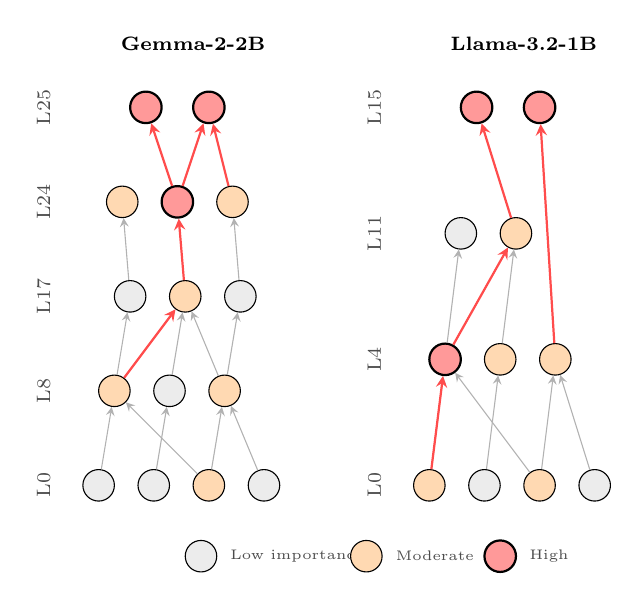
\begin{tikzpicture}[
  node distance=0.6cm and 1.2cm,
  feat/.style={circle, draw, minimum size=0.4cm, inner sep=0pt, font=\tiny},
  high/.style={feat, fill=red!40, thick},
  med/.style={feat, fill=orange!30},
  low/.style={feat, fill=gray!15},
  edge/.style={->, >=stealth, thin, gray!60},
  strong/.style={->, >=stealth, thick, red!70},
  label/.style={font=\scriptsize, text=black!70},
  ptitle/.style={font=\scriptsize\bfseries, anchor=south},
]

% --- Gemma-2-2B (left) ---
\node[ptitle] at (1.2, 5.4) {Gemma-2-2B};
\node[label, rotate=90] at (-0.7, 0) {L0};
\node[label, rotate=90] at (-0.7, 1.2) {L8};
\node[label, rotate=90] at (-0.7, 2.4) {L17};
\node[label, rotate=90] at (-0.7, 3.6) {L24};
\node[label, rotate=90] at (-0.7, 4.8) {L25};

\node[low] (g00) at (0, 0) {};
\node[low] (g01) at (0.7, 0) {};
\node[med] (g02) at (1.4, 0) {};
\node[low] (g03) at (2.1, 0) {};

\node[med] (g10) at (0.2, 1.2) {};
\node[low] (g11) at (0.9, 1.2) {};
\node[med] (g12) at (1.6, 1.2) {};

\node[low] (g20) at (0.4, 2.4) {};
\node[med] (g21) at (1.1, 2.4) {};
\node[low] (g22) at (1.8, 2.4) {};

\node[med] (g30) at (0.3, 3.6) {};
\node[high] (g31) at (1.0, 3.6) {};
\node[med] (g32) at (1.7, 3.6) {};

\node[high] (g40) at (0.6, 4.8) {};
\node[high] (g41) at (1.4, 4.8) {};

\draw[edge] (g00) -- (g10);
\draw[edge] (g01) -- (g11);
\draw[edge] (g02) -- (g10);
\draw[edge] (g02) -- (g12);
\draw[edge] (g03) -- (g12);
\draw[edge] (g10) -- (g20);
\draw[edge] (g11) -- (g21);
\draw[edge] (g12) -- (g21);
\draw[edge] (g12) -- (g22);
\draw[edge] (g20) -- (g30);
\draw[edge] (g22) -- (g32);
\draw[strong] (g10) -- (g21);
\draw[strong] (g21) -- (g31);
\draw[strong] (g31) -- (g40);
\draw[strong] (g31) -- (g41);
\draw[strong] (g32) -- (g41);

% --- Llama-3.2-1B (right) ---
\begin{scope}[xshift=4.2cm]
\node[ptitle] at (1.2, 5.4) {Llama-3.2-1B};
\node[label, rotate=90] at (-0.7, 0) {L0};
\node[label, rotate=90] at (-0.7, 1.6) {L4};
\node[label, rotate=90] at (-0.7, 3.2) {L11};
\node[label, rotate=90] at (-0.7, 4.8) {L15};

\node[med] (l00) at (0, 0) {};
\node[low] (l01) at (0.7, 0) {};
\node[med] (l02) at (1.4, 0) {};
\node[low] (l03) at (2.1, 0) {};

\node[high] (l10) at (0.2, 1.6) {};
\node[med] (l11) at (0.9, 1.6) {};
\node[med] (l12) at (1.6, 1.6) {};

\node[low] (l20) at (0.4, 3.2) {};
\node[med] (l21) at (1.1, 3.2) {};

\node[high] (l30) at (0.6, 4.8) {};
\node[high] (l31) at (1.4, 4.8) {};

\draw[edge] (l00) -- (l10);
\draw[edge] (l01) -- (l11);
\draw[edge] (l02) -- (l10);
\draw[edge] (l02) -- (l12);
\draw[edge] (l03) -- (l12);
\draw[edge] (l10) -- (l20);
\draw[edge] (l11) -- (l21);
\draw[strong] (l00) -- (l10);
\draw[strong] (l10) -- (l21);
\draw[strong] (l21) -- (l30);
\draw[strong] (l12) -- (l31);
\end{scope}

% Legend: single horizontal row, centred below both graphs
\node[low] (legL) at (1.3, -0.9) {};
\node[label, anchor=west] at (1.55, -0.9) {\tiny Low importance};
\node[med] (legM) at (3.4, -0.9) {};
\node[label, anchor=west] at (3.65, -0.9) {\tiny Moderate};
\node[high] (legH) at (5.1, -0.9) {};
\node[label, anchor=west] at (5.35, -0.9) {\tiny High};

\end{tikzpicture}
%
}
\DIFaddendFL \caption{Simplified attribution graphs for IOI: Gemma-2-2B (left) and Llama-3.2-1B (right).}
\label{fig:attribution_graph}
\end{figure}

Figure~\ref{fig:oracle_eff} summarises \DIFdelbegin \DIFdel{oracle efficiency across both
tasks and both models: the POMDP bar dominates random and greedy on IOI for
both architectures, and on Gemma it substantially exceeds the oracle envelope by exploiting steering actions that produce larger
per-feature KL than ablation alone.
}\DIFdelend \DIFaddbegin \DIFadd{bounded oracle efficiency for
the five ablation-only methods across IOI and multi-step tasks.  EAP
is the strongest baseline on both models; POMDP-abl is competitive
with the bandit on Gemma but falls behind on Llama, especially for
multi-step reasoning (discussed in Section~\ref{sec:multistep}).
}\DIFaddend 

\begin{figure}[H]
\centering
%DIF <  Auto-generated from experiment results.
\DIFdelbeginFL %DIFDELCMD < \begin{tikzpicture}
%DIFDELCMD < \begin{groupplot}[
%DIFDELCMD <     group style={
%DIFDELCMD <         group size=2 by 1,
%DIFDELCMD <         horizontal sep=0.5cm,
%DIFDELCMD <         ylabels at=edge left,
%DIFDELCMD <     },
%DIFDELCMD <     width=0.48\linewidth,
%DIFDELCMD <     height=6cm,
%DIFDELCMD <     ylabel={Oracle Efficiency (\%)},
%DIFDELCMD <     symbolic x coords={Random, Greedy, Bandit, POMDP},
%DIFDELCMD <     xtick=data,
%DIFDELCMD <     x tick label style={font=\scriptsize},
%DIFDELCMD <     y tick label style={font=\scriptsize},
%DIFDELCMD <     ylabel style={font=\scriptsize},
%DIFDELCMD <     title style={font=\scriptsize\bfseries},
%DIFDELCMD <     ymin=0,
%DIFDELCMD <     enlarge x limits=0.2,
%DIFDELCMD <     nodes near coords,
%DIFDELCMD <     nodes near coords style={font=\tiny},
%DIFDELCMD <     every node near coord/.append style={/pgf/number format/fixed,
%DIFDELCMD <         /pgf/number format/precision=1},
%DIFDELCMD <     legend style={
%DIFDELCMD <         font=\tiny,
%DIFDELCMD <         at={(0.5,-0.36)},
%DIFDELCMD <         anchor=north,
%DIFDELCMD <         legend columns=2
%DIFDELCMD <     },
%DIFDELCMD <     ymajorgrids=true,
%DIFDELCMD <     grid style={dashed, gray!30},
%DIFDELCMD < ]
%DIFDELCMD < 

%DIFDELCMD < \nextgroupplot[ybar, bar width=5pt, title={Gemma-2-2B}, ymax=1443]
%DIFDELCMD < \addplot[fill=blue!40, draw=blue!60] coordinates {
%DIFDELCMD <     (Random, 51.5) (Greedy, 66.9) (Bandit, 74.4) (POMDP, 1255.0)
%DIFDELCMD < };
%DIFDELCMD < 

%DIFDELCMD < \addplot[fill=red!40, draw=red!60] coordinates {
%DIFDELCMD <     (Random, 53.0) (Greedy, 79.4) (Bandit, 78.4) (POMDP, 983.0)
%DIFDELCMD < };
%DIFDELCMD < 

%DIFDELCMD < \legend{IOI, Multi-step}
%DIFDELCMD < 

%DIFDELCMD < \nextgroupplot[ybar, bar width=5pt, title={Llama-3.2-1B}, ymax=110]
%DIFDELCMD < \addplot[fill=blue!40, draw=blue!60] coordinates {
%DIFDELCMD <     (Random, 37.1) (Greedy, 40.8) (Bandit, 88.2) (POMDP, 90.6)
%DIFDELCMD < };
%DIFDELCMD < 

%DIFDELCMD < \addplot[fill=red!40, draw=red!60] coordinates {
%DIFDELCMD <     (Random, 51.6) (Greedy, 9.5) (Bandit, 76.4) (POMDP, 33.6)
%DIFDELCMD < };
%DIFDELCMD < 

%DIFDELCMD < \end{groupplot}
%DIFDELCMD < \end{tikzpicture}
%DIFDELCMD < %%%
\DIFdelendFL %DIF >  Auto-generated from experiment results (bounded oracle efficiency).
\DIFaddbeginFL 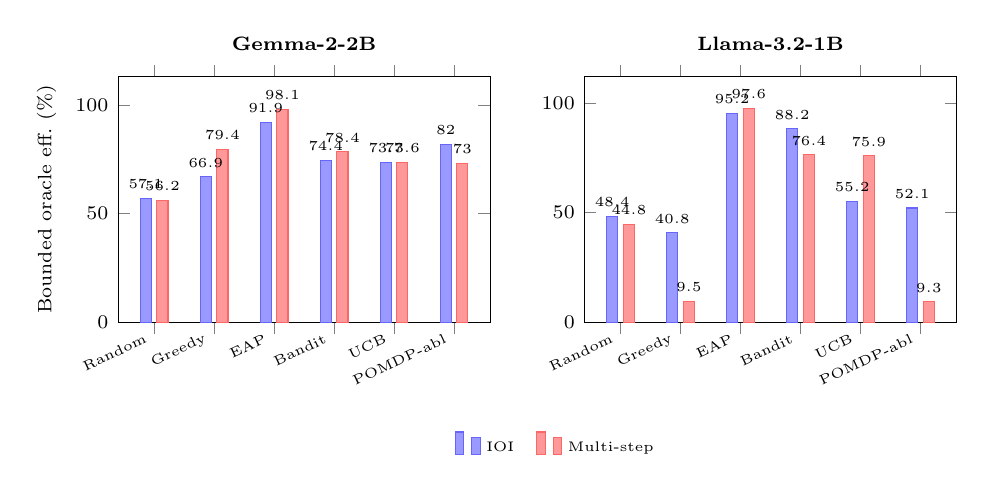
\begin{tikzpicture}
\begin{groupplot}[
    group style={group size=2 by 1, horizontal sep=1.2cm, ylabels at=edge left},
    width=0.52\columnwidth, height=4.7cm,
    ylabel={Bounded oracle eff.\ (\%)},
    symbolic x coords={Random, Greedy, EAP, Bandit, UCB, POMDP-abl},
    xtick=data,
    x tick label style={font=\tiny, rotate=25, anchor=east},
    y tick label style={font=\scriptsize},
    ylabel style={font=\scriptsize},
    title style={font=\scriptsize\bfseries},
    ymin=0,
    enlarge x limits=0.12,
    nodes near coords,
    nodes near coords style={font=\tiny},
    every node near coord/.append style={/pgf/number format/fixed,
        /pgf/number format/precision=1},
    legend image code/.code={\draw[#1] (0cm,-0.08cm) rectangle (0.30cm,0.12cm);},
    legend style={font=\tiny, legend columns=-1, draw=none,
        at={(1.18,-0.42)}, anchor=north,
        /tikz/every even column/.append style={column sep=6pt}},
]

\nextgroupplot[ybar, bar width=4pt, title={Gemma-2-2B}, ymax=113]
\addplot[fill=blue!40, draw=blue!60] coordinates { (Random, 57.1) (Greedy, 66.9) (EAP, 91.9) (Bandit, 74.4) (UCB, 73.7) (POMDP-abl, 82.0) };
\addplot[fill=red!40, draw=red!60] coordinates { (Random, 56.2) (Greedy, 79.4) (EAP, 98.1) (Bandit, 78.4) (UCB, 73.6) (POMDP-abl, 73.0) };
\legend{IOI, Multi-step}

\nextgroupplot[ybar, bar width=4pt, title={Llama-3.2-1B}, ymax=112]
\addplot[fill=blue!40, draw=blue!60] coordinates { (Random, 48.4) (Greedy, 40.8) (EAP, 95.2) (Bandit, 88.2) (UCB, 55.2) (POMDP-abl, 52.1) };
\addplot[fill=red!40, draw=red!60] coordinates { (Random, 44.8) (Greedy, 9.5) (EAP, 97.6) (Bandit, 76.4) (UCB, 75.9) (POMDP-abl, 9.3) };
\end{groupplot}
\end{tikzpicture}
\DIFaddendFL 

\DIFaddbeginFL \caption{\DIFaddFL{Bounded oracle efficiency (ablation-only) across IOI and
multi-step tasks for Gemma-2-2B (left) and Llama-3.2-1B (right).
By construction no method exceeds 100\%.}}
\label{fig:oracle_eff}
\end{figure}

\subsection{\DIFadd{Multi-Action Amplification: Relative Cumulative KL}}
\label{sec:rck}

\DIFadd{When the agent is allowed to choose the intervention }\emph{\DIFadd{type}}\DIFadd{, it
overwhelmingly selects feature steering, which scales a feature's
activation rather than zeroing it and can therefore produce KL
divergences far larger than ablation on the same feature.  Comparing
this multi-action cumulative KL to the ablation oracle yields
ratios well above 100\%, so it is not an oracle efficiency.  It is
reported under a distinct name, the Relative Cumulative KL
(RCK): the ratio of a multi-action method's cumulative KL to the
cumulative KL of the ablation oracle (Section~\ref{sec:setup}).  To
isolate how much of this amplification comes from selection
rather than from simply having the steering action, the full
POMDP is compared against action-matched baselines that share the identical
multi-action space (greedy+steer, bandit+steer, random+steer) and a
pure random-action control (Table~\ref{tab:rck}).
}

\begin{table}[H]
\centering
\caption{\DIFaddFL{Relative Cumulative KL (RCK, \%) of the multi-action POMDP
versus action-matched baselines, relative to the ablation oracle (100\%),
with bootstrap 95\% CIs over prompts.}}
\label{tab:rck}
{\small
\begin{tabular}{llcc}
\toprule
\textbf{\DIFaddFL{Model}} & \textbf{\DIFaddFL{Method}} & \textbf{\DIFaddFL{IOI RCK }[\DIFaddFL{95\% CI}]} & \textbf{\DIFaddFL{Multi-step RCK }[\DIFaddFL{95\% CI}]} \\
\midrule
\multirow{5}{*}{Gemma-2-2B}
 & \DIFaddFL{POMDP (multi) }& \DIFaddFL{1255 }[\DIFaddFL{974, 1671}] & \DIFaddFL{979 }[\DIFaddFL{792, 1374}] \\
 & \DIFaddFL{Bandit+steer  }& \DIFaddFL{1185 }[\DIFaddFL{780, 1797}] & \DIFaddFL{1209 }[\DIFaddFL{798, 1935}] \\
 & \DIFaddFL{Random+steer  }& \DIFaddFL{888 }[\DIFaddFL{672, 1182}]  & \DIFaddFL{737 }[\DIFaddFL{496, 1073}] \\
 & \DIFaddFL{Greedy+steer  }& \DIFaddFL{881 }[\DIFaddFL{605, 1675}]  & \DIFaddFL{1223 }[\DIFaddFL{707, 1907}] \\
 & \DIFaddFL{Random-action }& \DIFaddFL{371 }[\DIFaddFL{264, 528}]   & \DIFaddFL{249 }[\DIFaddFL{213, 296}] \\
\midrule
\multirow{5}{*}{Llama-3.2-1B}
 & \DIFaddFL{Bandit+steer  }& \DIFaddFL{1467 }[\DIFaddFL{329, 2848}] & \DIFaddFL{279 }[\DIFaddFL{203, 412}] \\
 & \DIFaddFL{Random+steer  }& \DIFaddFL{961 }[\DIFaddFL{181, 1907}]  & \DIFaddFL{381 }[\DIFaddFL{115, 868}] \\
 & \DIFaddFL{Random-action }& \DIFaddFL{429 }[\DIFaddFL{86, 811}]    & \DIFaddFL{164 }[\DIFaddFL{68, 340}] \\
 & \DIFaddFL{Greedy+steer  }& \DIFaddFL{353 }[\DIFaddFL{244, 482}]   & \DIFaddFL{140 }[\DIFaddFL{55, 293}] \\
 & \DIFaddFL{POMDP (multi) }& \DIFaddFL{91 }[\DIFaddFL{27, 320}]     & \DIFaddFL{34 }[\DIFaddFL{19, 56}] \\
\bottomrule
\end{tabular}
}
\end{table}

\DIFadd{The decomposition is revealing.  On Gemma, every steering-enabled
strategy, including random+steer (888\%), produces RCK far above
100\%, so the bulk of the amplification is attributable to the
steering action itself, not to which feature is selected.  The full
POMDP (1255\%) does sit at the top of the IOI ordering, indicating
that EFE selection adds a further margin over random steering, though the
action choice dominates.  On Llama the agent behaves very differently:
it mostly chooses ablation (70/100 actions, Section~\ref{sec:dynamics})
and its RCK is only 91\%, below the ablation oracle and well below
bandit+steer (1467\%).  This confirms that the figures above 100\% are a
property of the steering intervention rather than evidence that the
agent recovers more circuit structure than ablation-based methods; the
RCK scale must therefore not be read as a super-oracle discovery rate.
Figure~\ref{fig:rck} visualises the decomposition.
}

\begin{figure}[H]
\centering
%DIF >  Auto-generated: RCK (multi-action) vs ablation oracle (100% dashed line).
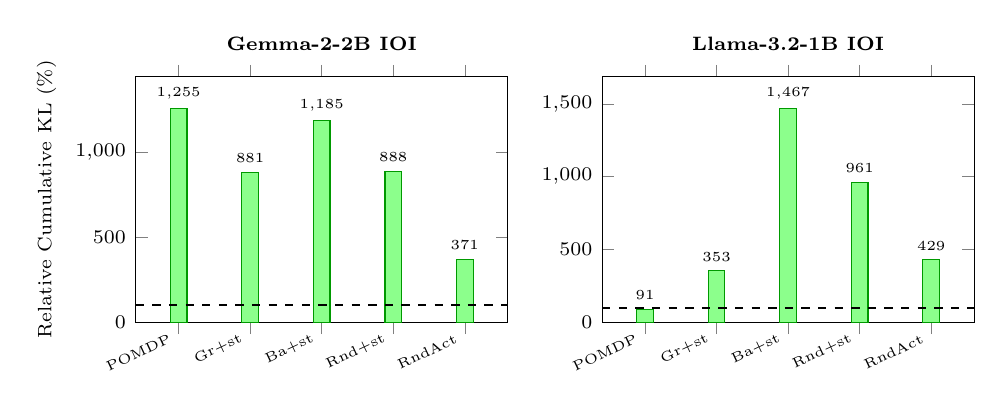
\begin{tikzpicture}
\begin{groupplot}[
    group style={group size=2 by 1, horizontal sep=1.2cm, ylabels at=edge left},
    width=0.52\columnwidth, height=4.7cm,
    ylabel={Relative Cumulative KL (\%)},
    symbolic x coords={POMDP, Gr+st, Ba+st, Rnd+st, RndAct},
    xtick=data,
    x tick label style={font=\tiny, rotate=25, anchor=east},
    y tick label style={font=\scriptsize},
    ylabel style={font=\scriptsize},
    title style={font=\scriptsize\bfseries},
    ymin=0, enlarge x limits=0.15,
    nodes near coords, nodes near coords style={font=\tiny},
    every node near coord/.append style={/pgf/number format/fixed,
        /pgf/number format/precision=0},
]

\nextgroupplot[ybar, bar width=6pt, title={Gemma-2-2B IOI}, ymax=1443]
\addplot[fill=green!45, draw=green!60!black] coordinates { (POMDP, 1255.0) (Gr+st, 881.1) (Ba+st, 1185.3) (Rnd+st, 888.2) (RndAct, 371.1) };
\draw[black, dashed, thick] ({rel axis cs:0,0}|-{axis cs:POMDP,100}) -- ({rel axis cs:1,0}|-{axis cs:POMDP,100});
\nextgroupplot[ybar, bar width=6pt, title={Llama-3.2-1B IOI}, ymax=1686]
\addplot[fill=green!45, draw=green!60!black] coordinates { (POMDP, 90.6) (Gr+st, 352.8) (Ba+st, 1466.5) (Rnd+st, 960.5) (RndAct, 429.0) };
\draw[black, dashed, thick] ({rel axis cs:0,0}|-{axis cs:POMDP,100}) -- ({rel axis cs:1,0}|-{axis cs:POMDP,100});
\end{groupplot}
\end{tikzpicture}

\DIFaddendFL \caption{\DIFdelbeginFL \DIFdelFL{Oracle efficiency across IOI and multi-step tasks for Gemma-2-2B }\DIFdelendFL \DIFaddbeginFL \DIFaddFL{Relative Cumulative KL of the multi-action POMDP against
action-matched baselines }\DIFaddendFL (\DIFdelbeginFL \DIFdelFL{left}\DIFdelendFL \DIFaddbeginFL \DIFaddFL{Gr+st, Ba+st, Rnd+st}\DIFaddendFL ) and \DIFdelbeginFL \DIFdelFL{Llama-3.2-1B }\DIFdelendFL \DIFaddbeginFL \DIFaddFL{a random-action
control }\DIFaddendFL (\DIFdelbeginFL \DIFdelFL{right}\DIFdelendFL \DIFaddbeginFL \DIFaddFL{RndAct}\DIFaddendFL )\DIFaddbeginFL \DIFaddFL{, relative to the ablation oracle (100\%, dashed)}\DIFaddendFL .}
\DIFdelbeginFL %DIFDELCMD < \label{fig:oracle_eff}
%DIFDELCMD < %%%
\DIFdelendFL \DIFaddbeginFL \label{fig:rck}
\DIFaddendFL \end{figure}

\subsection{Feature Steering \DIFaddbegin \DIFadd{and Causal Controllability}\DIFaddend }

Causal controllability is \DIFdelbegin \DIFdel{evaluated }\DIFdelend \DIFaddbegin \DIFadd{tested }\DIFaddend by scaling individual transcoder
feature activations \DIFdelbegin \DIFdel{at multipliers $m \in \{0, 2, 5, 10\}$ }\DIFdelend \DIFaddbegin \DIFadd{across a multiplier sweep
$m \in \{0, 1.5, 2, 3, 5, 10\}$ }\DIFaddend on 5 concept prompts with 10
\DIFdelbegin \DIFdel{features each.  Concept-level prediction-change
counts and maximum KL divergences are reported in
}\DIFdelend \DIFaddbegin \DIFadd{circuit-selected features each (50 features per model).  To separate
selectivity from out-of-distribution (OOD) effects of large
multipliers, a matched random-feature control of 10 random
active features per prompt is subjected to the identical sweep.  At
each multiplier, the number of top-token prediction changes
and the mean KL divergence are recorded for selected and control features
(}\DIFaddend Table~\ref{tab:steering}\DIFaddbegin \DIFadd{)}\DIFaddend .

\begin{table}[H]
\centering
\caption{Feature \DIFdelbeginFL \DIFdelFL{Steering Results}\DIFdelendFL \DIFaddbeginFL \DIFaddFL{steering dose--response: prediction changes
(selected / control, out of 50) and mean KL across the multiplier
sweep.  Circuit-selected features vs.\ a random-feature control.}\DIFaddendFL }
\label{tab:steering}
{\small
\DIFdelbeginFL %DIFDELCMD < \begin{tabular}{llccc}
%DIFDELCMD < %%%
\DIFdelendFL \DIFaddbeginFL \begin{tabular}{llcccccc}
\DIFaddendFL \toprule
\textbf{Model} & \textbf{\DIFdelbeginFL \DIFdelFL{Concept}\DIFdelendFL \DIFaddbeginFL \DIFaddFL{Quantity}\DIFaddendFL } & \textbf{\DIFdelbeginFL \DIFdelFL{$m$=5}\DIFdelendFL \DIFaddbeginFL \DIFaddFL{$m{=}0$}\DIFaddendFL } & \textbf{\DIFdelbeginFL \DIFdelFL{$m$=10}\DIFdelendFL \DIFaddbeginFL \DIFaddFL{$m{=}1.5$}\DIFaddendFL } & \textbf{\DIFdelbeginFL \DIFdelFL{Max KL}\DIFdelendFL \DIFaddbeginFL \DIFaddFL{$m{=}2$}\DIFaddendFL } \DIFaddbeginFL & \textbf{\DIFaddFL{$m{=}3$}} & \textbf{\DIFaddFL{$m{=}5$}} & \textbf{\DIFaddFL{$m{=}10$}} \DIFaddendFL \\
\midrule
\DIFdelbeginFL %DIFDELCMD < \multirow{5}{*}{Gemma-2-2B}
%DIFDELCMD <  %%%
\DIFdelendFL \DIFaddbeginFL \multirow{4}{*}{Gemma-2-2B}
 \DIFaddendFL & \DIFdelbeginFL \DIFdelFL{Golden Gate Br.}\DIFdelendFL \DIFaddbeginFL \DIFaddFL{Changes (sel.)   }\DIFaddendFL & 0/\DIFdelbeginFL \DIFdelFL{10  }\DIFdelendFL \DIFaddbeginFL \DIFaddFL{50 }\DIFaddendFL & 0/\DIFdelbeginFL \DIFdelFL{10  }\DIFdelendFL \DIFaddbeginFL \DIFaddFL{50 }\DIFaddendFL & \DIFdelbeginFL \DIFdelFL{0.078  }%DIFDELCMD < \\
%DIFDELCMD <  %%%
\DIFdelendFL \DIFaddbeginFL \DIFaddFL{1/50 }\DIFaddendFL & \DIFdelbeginFL \DIFdelFL{Eiffel Tower        }%DIFDELCMD < & %%%
\DIFdelendFL 2/\DIFdelbeginFL \DIFdelFL{10  }\DIFdelendFL \DIFaddbeginFL \DIFaddFL{50 }\DIFaddendFL & \DIFdelbeginFL \DIFdelFL{3/10  }\DIFdelendFL \DIFaddbeginFL \DIFaddFL{6/50 }\DIFaddendFL & \DIFdelbeginFL \DIFdelFL{1.061  }\DIFdelendFL \DIFaddbeginFL \DIFaddFL{11/50 }\DIFaddendFL \\
 & \DIFdelbeginFL \DIFdelFL{Mount Everest       }\DIFdelendFL \DIFaddbeginFL \DIFaddFL{Changes (ctrl.)  }\DIFaddendFL & 0/\DIFdelbeginFL \DIFdelFL{10  }\DIFdelendFL \DIFaddbeginFL \DIFaddFL{50 }\DIFaddendFL & 0/\DIFdelbeginFL \DIFdelFL{10  }\DIFdelendFL \DIFaddbeginFL \DIFaddFL{50 }\DIFaddendFL & \DIFdelbeginFL \DIFdelFL{0.045  }\DIFdelendFL \DIFaddbeginFL \DIFaddFL{1/50 }& \DIFaddFL{1/50 }& \DIFaddFL{2/50 }& \DIFaddFL{8/50 }\DIFaddendFL \\
 & \DIFdelbeginFL \DIFdelFL{Great Wall          }\DIFdelendFL \DIFaddbeginFL \DIFaddFL{Mean KL (sel.)   }\DIFaddendFL & \DIFdelbeginFL \DIFdelFL{3/10  }\DIFdelendFL \DIFaddbeginFL \DIFaddFL{0.001 }\DIFaddendFL & \DIFdelbeginFL \DIFdelFL{4/10  }\DIFdelendFL \DIFaddbeginFL \DIFaddFL{0.000 }\DIFaddendFL & \DIFdelbeginFL \DIFdelFL{3.455  }\DIFdelendFL \DIFaddbeginFL \DIFaddFL{0.002 }& \DIFaddFL{0.007 }& \DIFaddFL{0.039 }& \DIFaddFL{0.367 }\DIFaddendFL \\
 & \DIFdelbeginFL \DIFdelFL{Statue of Liberty   }\DIFdelendFL \DIFaddbeginFL \DIFaddFL{Mean KL (ctrl.)  }\DIFaddendFL & \DIFdelbeginFL \DIFdelFL{0/10  }\DIFdelendFL \DIFaddbeginFL \DIFaddFL{0.001 }\DIFaddendFL & \DIFdelbeginFL \DIFdelFL{1/10  }\DIFdelendFL \DIFaddbeginFL \DIFaddFL{0.000 }\DIFaddendFL & \DIFdelbeginFL \DIFdelFL{0.157  }\DIFdelendFL \DIFaddbeginFL \DIFaddFL{0.001 }& \DIFaddFL{0.005 }& \DIFaddFL{0.020 }& \DIFaddFL{0.086 }\DIFaddendFL \\
\midrule
\DIFdelbeginFL %DIFDELCMD < \multirow{5}{*}{Llama-3.2-1B}
%DIFDELCMD <  %%%
\DIFdelendFL \DIFaddbeginFL \multirow{4}{*}{Llama-3.2-1B}
 \DIFaddendFL & \DIFdelbeginFL \DIFdelFL{Golden Gate Br.}\DIFdelendFL \DIFaddbeginFL \DIFaddFL{Changes (sel.)   }\DIFaddendFL & 0/\DIFdelbeginFL \DIFdelFL{10  }\DIFdelendFL \DIFaddbeginFL \DIFaddFL{50 }\DIFaddendFL & \DIFaddbeginFL \DIFaddFL{0/50 }& \DIFaddFL{0/50 }& \DIFaddendFL 1/\DIFdelbeginFL \DIFdelFL{10  }\DIFdelendFL \DIFaddbeginFL \DIFaddFL{50 }\DIFaddendFL & \DIFdelbeginFL \DIFdelFL{1.514  }\DIFdelendFL \DIFaddbeginFL \DIFaddFL{1/50 }& \DIFaddFL{9/50 }\DIFaddendFL \\
 & \DIFdelbeginFL \DIFdelFL{Eiffel Tower        }\DIFdelendFL \DIFaddbeginFL \DIFaddFL{Changes (ctrl.)  }\DIFaddendFL & 0/\DIFdelbeginFL \DIFdelFL{10  }\DIFdelendFL \DIFaddbeginFL \DIFaddFL{50 }\DIFaddendFL & 0/\DIFdelbeginFL \DIFdelFL{10  }\DIFdelendFL \DIFaddbeginFL \DIFaddFL{50 }\DIFaddendFL & \DIFdelbeginFL \DIFdelFL{0.779  }%DIFDELCMD < \\
%DIFDELCMD <  %%%
\DIFdelendFL \DIFaddbeginFL \DIFaddFL{0/50 }\DIFaddendFL & \DIFdelbeginFL \DIFdelFL{Mount Everest       }%DIFDELCMD < & %%%
\DIFdelendFL 0/\DIFdelbeginFL \DIFdelFL{10  }\DIFdelendFL \DIFaddbeginFL \DIFaddFL{50 }\DIFaddendFL & 0/\DIFdelbeginFL \DIFdelFL{10  }\DIFdelendFL \DIFaddbeginFL \DIFaddFL{50 }\DIFaddendFL & \DIFdelbeginFL \DIFdelFL{0.988  }\DIFdelendFL \DIFaddbeginFL \DIFaddFL{6/50 }\DIFaddendFL \\
 & \DIFdelbeginFL \DIFdelFL{Great Wall          }\DIFdelendFL \DIFaddbeginFL \DIFaddFL{Mean KL (sel.)   }\DIFaddendFL & \DIFdelbeginFL \DIFdelFL{2/10  }\DIFdelendFL \DIFaddbeginFL \DIFaddFL{0.005 }\DIFaddendFL & \DIFdelbeginFL \DIFdelFL{5/10  }\DIFdelendFL \DIFaddbeginFL \DIFaddFL{0.001 }\DIFaddendFL & \DIFdelbeginFL \DIFdelFL{0.556  }\DIFdelendFL \DIFaddbeginFL \DIFaddFL{0.003 }& \DIFaddFL{0.011 }& \DIFaddFL{0.043 }& \DIFaddFL{0.232 }\DIFaddendFL \\
 & \DIFdelbeginFL \DIFdelFL{Statue of Liberty   }\DIFdelendFL \DIFaddbeginFL \DIFaddFL{Mean KL (ctrl.)  }\DIFaddendFL & \DIFdelbeginFL \DIFdelFL{0/10  }\DIFdelendFL \DIFaddbeginFL \DIFaddFL{0.001 }\DIFaddendFL & \DIFdelbeginFL \DIFdelFL{3/10  }\DIFdelendFL \DIFaddbeginFL \DIFaddFL{0.000 }\DIFaddendFL & \DIFdelbeginFL \DIFdelFL{1.828  }\DIFdelendFL \DIFaddbeginFL \DIFaddFL{0.000 }& \DIFaddFL{0.002 }& \DIFaddFL{0.010 }& \DIFaddFL{0.120 }\DIFaddendFL \\
\bottomrule
\end{tabular}%
}
\end{table}

\DIFdelbegin \DIFdel{Cells show $n/10$ top-token prediction changes.  The Great Wall prompt
proves most steerable on both models (4/10 }\DIFdelend \DIFaddbegin \DIFadd{Two effects are visible.  First, manipulability (H2a): both KL
and prediction-change rate rise monotonically with the multiplier, and
}\DIFaddend at $m{=}10$ \DIFdelbegin \DIFdel{for Gemma, 5/10 for Llama) , while Mount Everest shows no changes on either, suggesting concept-dependent robustness.  Total prediction changes:
13/100 for Gemma, }\DIFdelend \DIFaddbegin \DIFadd{the selected-feature change rate (}\DIFaddend 11/\DIFdelbegin \DIFdel{100 for Llama. }\DIFdelend \DIFaddbegin \DIFadd{50 on Gemma, 9/50 on
Llama) is far above the per-token chance rate (a one-sided binomial
test against chance gives $p<10^{-8}$).  Steering transcoder features
causally and dose-dependently moves the output distribution.
Second, and more cautiously, selectivity (H2b): circuit-selected
features carry higher mean KL than random controls at large
multipliers (for example, $0.367$ versus $0.086$ on Gemma at $m{=}10$), but the
prediction-change advantage is small (11 versus 8 on Gemma, 9
versus 6 on Llama).  A one-sided Fisher exact test on the
selected-versus-control change counts is not significant, either at
$m{=}10$ or pooled over $m\geq 2$.  Circuit-selected features are thus only
marginally, and not significantly, more controllable than random
active features at the prediction level, and the largest
multipliers push activations off-distribution; the steering result
should accordingly be read as a controllability demonstration, not as proof of
privileged selectivity.
}\DIFaddend 

\DIFaddbegin \DIFadd{A complementary view of the largest multipliers confirms that steering
amplifies coherent concepts rather than merely degrading the model. As
the multiplier increases from $0$ to $10$, the mean probability mass on
the steered top-1 token remains high (approximately $0.43$ on Gemma).
At the same time, the set of distinct dominant tokens broadens from 5 to 11 and
increasingly features content tokens associated with the steered
concepts (for example geographic and landmark tokens) rather than
collapsing onto generic function words. This indicates that large
multipliers redirect the prediction toward specific concepts rather than
producing undifferentiated noise.
}

\DIFaddend The per-multiplier KL response \DIFdelbegin \DIFdel{for each concept is visualised as a
heatmap }\DIFdelend \DIFaddbegin \DIFadd{is visualised }\DIFaddend in
Figure~\ref{fig:steering}\DIFdelbegin \DIFdel{, which highlights that the
steerability gap between concepts grows with the steering multiplier
and is broadly consistent across the two model families}\DIFdelend .

\begin{figure}[H]
\centering
% Auto-generated from experiment results.
\DIFdelbeginFL %DIFDELCMD < \begin{tikzpicture}
%DIFDELCMD < \begin{groupplot}[
%DIFDELCMD <     group style={
%DIFDELCMD <         group size=2 by 1,
%DIFDELCMD <         horizontal sep=0.5cm,
%DIFDELCMD <         ylabels at=edge left,
%DIFDELCMD <     },
%DIFDELCMD <     width=0.48\linewidth,
%DIFDELCMD <     height=6cm,
%DIFDELCMD <     xlabel={Steering multiplier $m$},
%DIFDELCMD <     ylabel={Mean KL divergence},
%DIFDELCMD <     x label style={font=\scriptsize},
%DIFDELCMD <     y label style={font=\scriptsize},
%DIFDELCMD <     tick label style={font=\scriptsize},
%DIFDELCMD <     title style={font=\scriptsize\bfseries},
%DIFDELCMD <     legend style={
%DIFDELCMD <         font=\tiny,
%DIFDELCMD <         at={(0.5,-0.33)},
%DIFDELCMD <         anchor=north,
%DIFDELCMD <         legend columns=3
%DIFDELCMD <     },
%DIFDELCMD <     xtick={0,2,5,10},
%DIFDELCMD <     ymajorgrids=true,
%DIFDELCMD <     grid style={dashed, gray!30},
%DIFDELCMD < ]
%DIFDELCMD < 

%DIFDELCMD < \nextgroupplot[title={Gemma-2-2B}]
%DIFDELCMD < \addplot[blue, thick, mark=*] coordinates { (0.0,0.000249) (2.0,0.000571) (5.0,0.004278) (10.0,0.010184) };
%DIFDELCMD < \addplot[red, thick, mark=*] coordinates { (0.0,0.001281) (2.0,0.001446) (5.0,0.024365) (10.0,0.162296) };
%DIFDELCMD < \addplot[green!60!black, thick, mark=*] coordinates { (0.0,0.000136) (2.0,0.000102) (5.0,0.002692) (10.0,0.008660) };
%DIFDELCMD < \addplot[purple, thick, mark=*] coordinates { (0.0,0.003460) (2.0,0.003683) (5.0,0.063126) (10.0,0.455828) };
%DIFDELCMD < \addplot[brown, thick, mark=*] coordinates { (0.0,0.000386) (2.0,0.000623) (5.0,0.006513) (10.0,0.024498) };
%DIFDELCMD < \legend{Golden Gate Bridge, Eiffel Tower, Mount Everest, Great Wall of China, Statue of Liberty}
%DIFDELCMD < 

%DIFDELCMD < \nextgroupplot[title={Llama-3.2-1B}]
%DIFDELCMD < \addplot[blue, thick, mark=*] coordinates { (0.0,0.003609) (2.0,0.001486) (5.0,0.029852) (10.0,0.193760) };
%DIFDELCMD < \addplot[red, thick, mark=*] coordinates { (0.0,0.000730) (2.0,0.000461) (5.0,0.008967) (10.0,0.080968) };
%DIFDELCMD < \addplot[green!60!black, thick, mark=*] coordinates { (0.0,0.001963) (2.0,0.001359) (5.0,0.010197) (10.0,0.123166) };
%DIFDELCMD < \addplot[purple, thick, mark=*] coordinates { (0.0,0.011569) (2.0,0.006607) (5.0,0.087774) (10.0,0.143479) };
%DIFDELCMD < \addplot[brown, thick, mark=*] coordinates { (0.0,0.007696) (2.0,0.003893) (5.0,0.065916) (10.0,0.446384) };
%DIFDELCMD < 

%DIFDELCMD < \end{groupplot}
%DIFDELCMD < \end{tikzpicture}
%DIFDELCMD < %%%
\DIFdelendFL \DIFaddbeginFL 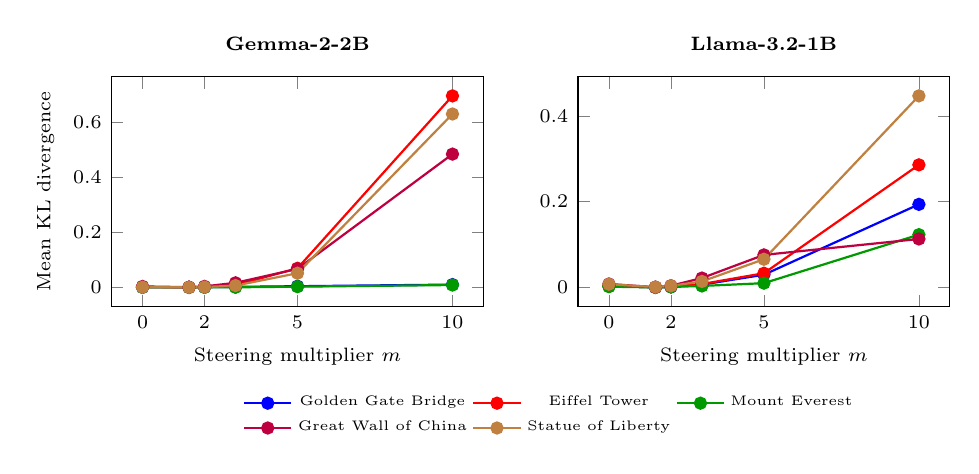
\begin{tikzpicture}
\begin{groupplot}[
    group style={
        group size=2 by 1,
        horizontal sep=1.2cm,
        ylabels at=edge left,
    },
    width=0.52\columnwidth,
    height=4.5cm,
    xlabel={Steering multiplier $m$},
    ylabel={Mean KL divergence},
    x label style={font=\scriptsize},
    y label style={font=\scriptsize},
    tick label style={font=\scriptsize},
    title style={font=\scriptsize\bfseries},
    legend style={
        font=\tiny, draw=none,
        at={(1.18,-0.34)},
        anchor=north,
        legend columns=3
    },
    xtick={0,2,5,10},
]

\nextgroupplot[title={Gemma-2-2B}]
\addplot[blue, thick, mark=*] coordinates { (0.0,0.000249) (1.5,0.000130) (2.0,0.000571) (3.0,0.001968) (5.0,0.004278) (10.0,0.010184) };
\addplot[red, thick, mark=*] coordinates { (0.0,0.001352) (1.5,0.000352) (2.0,0.001520) (3.0,0.008043) (5.0,0.069690) (10.0,0.697324) };
\addplot[green!60!black, thick, mark=*] coordinates { (0.0,0.000136) (1.5,0.000026) (2.0,0.000102) (3.0,0.000365) (5.0,0.002692) (10.0,0.008660) };
\addplot[purple, thick, mark=*] coordinates { (0.0,0.003536) (1.5,0.000906) (2.0,0.003722) (3.0,0.016692) (5.0,0.067487) (10.0,0.485322) };
\addplot[brown, thick, mark=*] coordinates { (0.0,0.000898) (1.5,0.000303) (2.0,0.001338) (3.0,0.006564) (5.0,0.051704) (10.0,0.631355) };
\legend{Golden Gate Bridge, Eiffel Tower, Mount Everest, Great Wall of China, Statue of Liberty}

\nextgroupplot[title={Llama-3.2-1B}]
\addplot[blue, thick, mark=*] coordinates { (0.0,0.003609) (1.5,0.000365) (2.0,0.001486) (3.0,0.006794) (5.0,0.029852) (10.0,0.193760) };
\addplot[red, thick, mark=*] coordinates { (0.0,0.003216) (1.5,0.000556) (2.0,0.002070) (3.0,0.008155) (5.0,0.033345) (10.0,0.285773) };
\addplot[green!60!black, thick, mark=*] coordinates { (0.0,0.001963) (1.5,0.000378) (2.0,0.001359) (3.0,0.003709) (5.0,0.010197) (10.0,0.123166) };
\addplot[purple, thick, mark=*] coordinates { (0.0,0.008333) (1.5,0.000816) (2.0,0.004294) (3.0,0.022110) (5.0,0.076030) (10.0,0.113099) };
\addplot[brown, thick, mark=*] coordinates { (0.0,0.007696) (1.5,0.001065) (2.0,0.003893) (3.0,0.014201) (5.0,0.065916) (10.0,0.446384) };

\end{groupplot}
\end{tikzpicture}
\DIFaddendFL 

\caption{Mean KL divergence across steering multipliers for five
concept prompts on both models.}
\label{fig:steering}
\end{figure}

\subsection{Active Discovery Dynamics}
\DIFaddbegin \label{sec:dynamics}
\DIFaddend 

The POMDP agent maintains explicit beliefs over three hidden state
factors and updates them after each intervention.  Across IOI prompts,
\DIFdelbegin \DIFdel{the agent's }\DIFdelend total belief entropy decreases \DIFdelbegin \DIFdel{monotonically over the intervention }\DIFdelend \DIFaddbegin \DIFadd{over the }\DIFaddend budget, indicating \DIFdelbegin \DIFdel{genuine }\DIFdelend information
accumulation about circuit structure.  \DIFaddbegin \DIFadd{The online learning of the
observation model itself also converges: the mean per-step $L_1$ drift
of the learned KL-likelihood matrix, $\|A_t - A_{t-1}\|_1$, decreases
monotonically over the budget (Figure~\ref{fig:aconv}), roughly halving
between the first and last update on Gemma IOI (from $1.03\times10^{-3}$
to $5.0\times10^{-4}$).  The Dirichlet posterior over the observation
model thus stabilises as evidence accumulates, rather than oscillating.
}\DIFaddend 

\DIFdelbegin \DIFdel{The agent selects from three intervention types at each step}\DIFdelend \DIFaddbegin \begin{figure}[H]
\centering
%DIF >  Auto-generated: A-matrix online convergence (mean L1 drift per step).
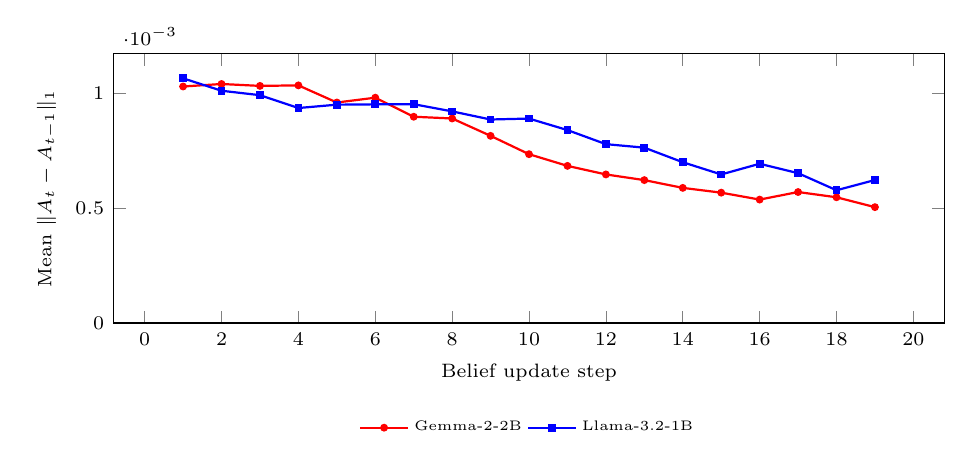
\begin{tikzpicture}
\begin{axis}[
    width=\columnwidth, height=5cm,
    xlabel={Belief update step}, ylabel={Mean $\|A_t-A_{t-1}\|_1$},
    x label style={font=\scriptsize}, y label style={font=\scriptsize},
    tick label style={font=\scriptsize},
    legend style={font=\tiny, legend columns=-1, draw=none,
        at={(0.5,-0.32)}, anchor=north},
    ymin=0,
]

\addplot[red, thick, mark=*, mark size=1pt] coordinates { (1,1.028281e-03) (2,1.039235e-03) (3,1.030940e-03) (4,1.033210e-03) (5,9.586966e-04) (6,9.796875e-04) (7,8.968510e-04) (8,8.892721e-04) (9,8.137831e-04) (10,7.340020e-04) (11,6.832358e-04) (12,6.460141e-04) (13,6.213705e-04) (14,5.875674e-04) (15,5.668197e-04) (16,5.367225e-04) (17,5.695627e-04) (18,5.467266e-04) (19,5.038578e-04) };
\addplot[blue, thick, mark=square*, mark size=1pt] coordinates { (1,1.063762e-03) (2,1.009849e-03) (3,9.905962e-04) (4,9.347575e-04) (5,9.492890e-04) (6,9.507243e-04) (7,9.513819e-04) (8,9.200837e-04) (9,8.848640e-04) (10,8.889142e-04) (11,8.388198e-04) (12,7.777137e-04) (13,7.624398e-04) (14,6.991302e-04) (15,6.459326e-04) (16,6.924570e-04) (17,6.515450e-04) (18,5.772606e-04) (19,6.217703e-04) };
\legend{Gemma-2-2B, Llama-3.2-1B}

\end{axis}
\end{tikzpicture}

\caption{\DIFaddFL{Online convergence of the learned observation model: mean
per-step $L_1$ drift of the KL-likelihood matrix across IOI prompts.}}
\label{fig:aconv}
\end{figure}

\DIFadd{The agent's action selection differs sharply between architectures,
which explains the RCK contrast in Section~\ref{sec:rck}}\DIFaddend .  On Gemma
IOI, ablation is selected first \DIFdelbegin \DIFdel{(step~0) }\DIFdelend for exploration, after which the agent
transitions to predominantly feature steering (94/100 steps\DIFdelbegin \DIFdel{) and }\DIFdelend \DIFaddbegin \DIFadd{; 94/95
post-first-step) with }\DIFaddend occasional activation patching (1/100\DIFdelbegin \DIFdel{steps).  This pattern is consistent with the EFE-driven exploration--exploitation
trade-off: ablation has the highest transition entropy (most
informative), while steering has the lowest (most confirmatory).  The agent's growing confidence in its importance estimates drives the
shift from exploratory to confirmatory interventions; the
}\DIFdelend \DIFaddbegin \DIFadd{).  On
Llama IOI the agent is far more conservative, choosing ablation for
70/100 steps and steering only 28/100, so its cumulative KL stays
near the ablation scale rather than amplifying.  The }\DIFaddend step-by-step
action distribution for both models is shown in
Figure~\ref{fig:action_dist}.  \DIFaddbegin \DIFadd{This action-policy divergence, rather
than any difference in feature ranking, is what drives the very
different RCK values across the two models.
}\DIFaddend 

\DIFdelbegin %DIFDELCMD < \begin{figure*}[t]
%DIFDELCMD < %%%
\DIFdelendFL \DIFaddbeginFL \begin{figure}[H]
\DIFaddendFL \centering
% Auto-generated by generate_figure_data.py
\DIFdelbeginFL %DIFDELCMD < \begin{tikzpicture}
%DIFDELCMD < \begin{groupplot}[
%DIFDELCMD <   group style={group size=2 by 2, horizontal sep=0.5cm, vertical sep=2.5cm},
%DIFDELCMD <   width=0.48\linewidth, height=5cm,
%DIFDELCMD <   xlabel={Step}, ylabel={Proportion},
%DIFDELCMD <   x label style={font=\scriptsize},
%DIFDELCMD <   y label style={font=\scriptsize},
%DIFDELCMD <   tick label style={font=\scriptsize},
%DIFDELCMD <   title style={font=\scriptsize\bfseries},
%DIFDELCMD <   ymin=0, ymax=1,
%DIFDELCMD <   legend style={at={(0.5,-0.25)}, anchor=north, legend columns=3, font=\tiny},
%DIFDELCMD <   ymajorgrids=true,
%DIFDELCMD <   grid style={dashed, gray!30},
%DIFDELCMD < ]
%DIFDELCMD < \nextgroupplot[title={Gemma IOI}, ybar stacked, bar width=3pt]
%DIFDELCMD < \addplot[fill=blue!70, draw=none] coordinates {(1,1.000) (2,0.000) (3,0.000) (4,0.000) (5,0.000) (6,0.000) (7,0.000) (8,0.000) (9,0.000) (10,0.000) (11,0.000) (12,0.000) (13,0.000) (14,0.000) (15,0.000) (16,0.000) (17,0.000) (18,0.000) (19,0.000) (20,0.000)};
%DIFDELCMD < \addplot[fill=orange!80, draw=none] coordinates {(1,0.000) (2,0.000) (3,0.000) (4,0.000) (5,0.000) (6,0.000) (7,0.000) (8,0.000) (9,0.000) (10,0.000) (11,0.000) (12,0.000) (13,0.000) (14,0.000) (15,0.000) (16,0.000) (17,0.000) (18,0.000) (19,0.000) (20,0.200)};
%DIFDELCMD < \addplot[fill=green!60!black, draw=none] coordinates {(1,0.000) (2,1.000) (3,1.000) (4,1.000) (5,1.000) (6,1.000) (7,1.000) (8,1.000) (9,1.000) (10,1.000) (11,1.000) (12,1.000) (13,1.000) (14,1.000) (15,1.000) (16,1.000) (17,1.000) (18,1.000) (19,1.000) (20,0.800)};
%DIFDELCMD < \nextgroupplot[title={Gemma Multi-step}, ybar stacked, bar width=3pt]
%DIFDELCMD < \addplot[fill=blue!70, draw=none] coordinates {(1,0.667) (2,0.000) (3,0.000) (4,0.000) (5,0.000) (6,0.000) (7,0.000) (8,0.000) (9,0.000) (10,0.000) (11,0.000) (12,0.000) (13,0.000) (14,0.000) (15,0.000) (16,0.000) (17,0.000) (18,0.000) (19,0.000) (20,0.333)};
%DIFDELCMD < \addplot[fill=orange!80, draw=none] coordinates {(1,0.000) (2,0.000) (3,0.000) (4,0.000) (5,0.000) (6,0.000) (7,0.000) (8,0.000) (9,0.000) (10,0.000) (11,0.000) (12,0.000) (13,0.000) (14,0.000) (15,0.000) (16,0.000) (17,0.000) (18,0.000) (19,0.000) (20,0.000)};
%DIFDELCMD < \addplot[fill=green!60!black, draw=none] coordinates {(1,0.333) (2,1.000) (3,1.000) (4,1.000) (5,1.000) (6,1.000) (7,1.000) (8,1.000) (9,1.000) (10,1.000) (11,1.000) (12,1.000) (13,1.000) (14,1.000) (15,1.000) (16,1.000) (17,1.000) (18,1.000) (19,1.000) (20,0.667)};
%DIFDELCMD < \nextgroupplot[title={Llama IOI}, ybar stacked, bar width=3pt]
%DIFDELCMD < \addplot[fill=blue!70, draw=none] coordinates {(1,1.000) (2,1.000) (3,0.800) (4,0.800) (5,0.800) (6,0.800) (7,0.600) (8,0.600) (9,0.600) (10,0.600) (11,0.600) (12,0.600) (13,0.600) (14,0.600) (15,0.600) (16,0.600) (17,0.600) (18,0.600) (19,0.800) (20,0.800)};
%DIFDELCMD < \addplot[fill=orange!80, draw=none] coordinates {(1,0.000) (2,0.000) (3,0.000) (4,0.000) (5,0.000) (6,0.000) (7,0.000) (8,0.000) (9,0.000) (10,0.000) (11,0.000) (12,0.000) (13,0.000) (14,0.000) (15,0.000) (16,0.000) (17,0.000) (18,0.200) (19,0.000) (20,0.200)};
%DIFDELCMD < \addplot[fill=green!60!black, draw=none] coordinates {(1,0.000) (2,0.000) (3,0.200) (4,0.200) (5,0.200) (6,0.200) (7,0.400) (8,0.400) (9,0.400) (10,0.400) (11,0.400) (12,0.400) (13,0.400) (14,0.400) (15,0.400) (16,0.400) (17,0.400) (18,0.200) (19,0.200) (20,0.000)};
%DIFDELCMD < \nextgroupplot[title={Llama Multi-step}, ybar stacked, bar width=3pt]
%DIFDELCMD < \addplot[fill=blue!70, draw=none] coordinates {(1,1.000) (2,0.667) (3,0.667) (4,0.333) (5,0.667) (6,0.667) (7,0.667) (8,0.667) (9,0.667) (10,0.667) (11,0.667) (12,0.667) (13,0.667) (14,0.667) (15,0.667) (16,0.667) (17,0.667) (18,0.667) (19,0.667) (20,1.000)};
%DIFDELCMD < \addplot[fill=orange!80, draw=none] coordinates {(1,0.000) (2,0.000) (3,0.000) (4,0.000) (5,0.000) (6,0.000) (7,0.000) (8,0.000) (9,0.000) (10,0.000) (11,0.000) (12,0.000) (13,0.000) (14,0.000) (15,0.000) (16,0.000) (17,0.000) (18,0.000) (19,0.333) (20,0.000)};
%DIFDELCMD < \addplot[fill=green!60!black, draw=none] coordinates {(1,0.000) (2,0.333) (3,0.333) (4,0.667) (5,0.333) (6,0.333) (7,0.333) (8,0.333) (9,0.333) (10,0.333) (11,0.333) (12,0.333) (13,0.333) (14,0.333) (15,0.333) (16,0.333) (17,0.333) (18,0.333) (19,0.000) (20,0.000)};
%DIFDELCMD < \legend{Ablation, Patching, Steering}
%DIFDELCMD < \end{groupplot}
%DIFDELCMD < \end{tikzpicture}
%DIFDELCMD < %%%
\DIFdelendFL \DIFaddbeginFL 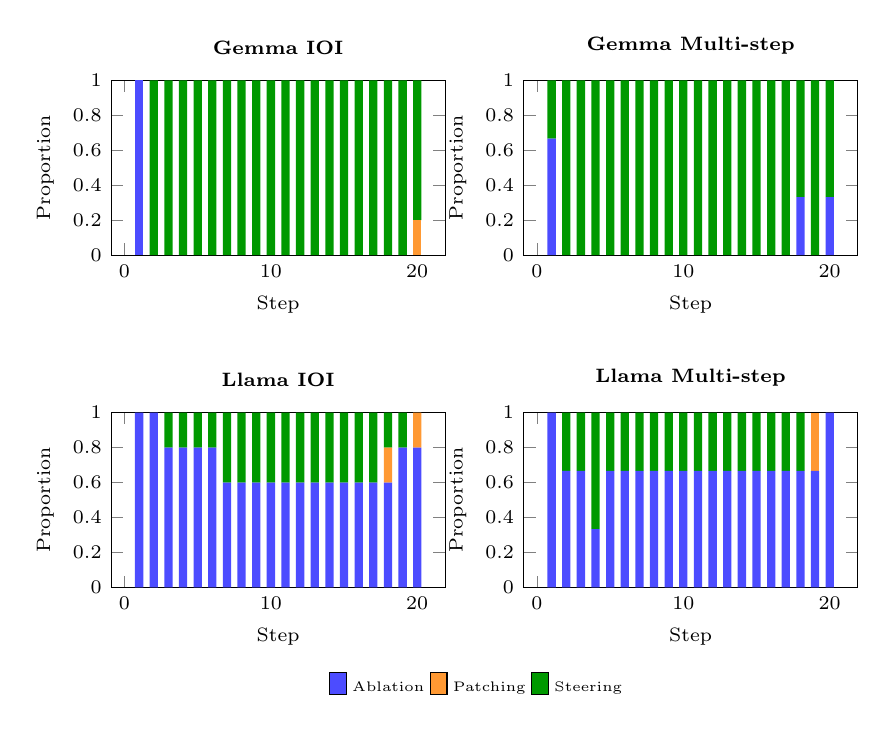
\begin{tikzpicture}
\begin{groupplot}[
  group style={group size=2 by 2, horizontal sep=1.0cm, vertical sep=2.0cm},
  width=0.48\columnwidth, height=3.8cm,
  xlabel={Step}, ylabel={Proportion},
  x label style={font=\scriptsize},
  y label style={font=\scriptsize},
  tick label style={font=\scriptsize},
  title style={font=\scriptsize\bfseries},
  ymin=0, ymax=1,
  legend image code/.code={\draw[#1] (0cm,-0.08cm) rectangle (0.30cm,0.12cm);},
  legend style={at={(1.1,-0.45)}, anchor=north, legend columns=-1, draw=none, font=\tiny},
]
\nextgroupplot[title={Gemma IOI}, ybar stacked, bar width=3pt]
\addplot[fill=blue!70, draw=none] coordinates {(1,1.000) (2,0.000) (3,0.000) (4,0.000) (5,0.000) (6,0.000) (7,0.000) (8,0.000) (9,0.000) (10,0.000) (11,0.000) (12,0.000) (13,0.000) (14,0.000) (15,0.000) (16,0.000) (17,0.000) (18,0.000) (19,0.000) (20,0.000)};
\addplot[fill=orange!80, draw=none] coordinates {(1,0.000) (2,0.000) (3,0.000) (4,0.000) (5,0.000) (6,0.000) (7,0.000) (8,0.000) (9,0.000) (10,0.000) (11,0.000) (12,0.000) (13,0.000) (14,0.000) (15,0.000) (16,0.000) (17,0.000) (18,0.000) (19,0.000) (20,0.200)};
\addplot[fill=green!60!black, draw=none] coordinates {(1,0.000) (2,1.000) (3,1.000) (4,1.000) (5,1.000) (6,1.000) (7,1.000) (8,1.000) (9,1.000) (10,1.000) (11,1.000) (12,1.000) (13,1.000) (14,1.000) (15,1.000) (16,1.000) (17,1.000) (18,1.000) (19,1.000) (20,0.800)};
\nextgroupplot[title={Gemma Multi-step}, ybar stacked, bar width=3pt]
\addplot[fill=blue!70, draw=none] coordinates {(1,0.667) (2,0.000) (3,0.000) (4,0.000) (5,0.000) (6,0.000) (7,0.000) (8,0.000) (9,0.000) (10,0.000) (11,0.000) (12,0.000) (13,0.000) (14,0.000) (15,0.000) (16,0.000) (17,0.000) (18,0.333) (19,0.000) (20,0.333)};
\addplot[fill=orange!80, draw=none] coordinates {(1,0.000) (2,0.000) (3,0.000) (4,0.000) (5,0.000) (6,0.000) (7,0.000) (8,0.000) (9,0.000) (10,0.000) (11,0.000) (12,0.000) (13,0.000) (14,0.000) (15,0.000) (16,0.000) (17,0.000) (18,0.000) (19,0.000) (20,0.000)};
\addplot[fill=green!60!black, draw=none] coordinates {(1,0.333) (2,1.000) (3,1.000) (4,1.000) (5,1.000) (6,1.000) (7,1.000) (8,1.000) (9,1.000) (10,1.000) (11,1.000) (12,1.000) (13,1.000) (14,1.000) (15,1.000) (16,1.000) (17,1.000) (18,0.667) (19,1.000) (20,0.667)};
\nextgroupplot[title={Llama IOI}, ybar stacked, bar width=3pt]
\addplot[fill=blue!70, draw=none] coordinates {(1,1.000) (2,1.000) (3,0.800) (4,0.800) (5,0.800) (6,0.800) (7,0.600) (8,0.600) (9,0.600) (10,0.600) (11,0.600) (12,0.600) (13,0.600) (14,0.600) (15,0.600) (16,0.600) (17,0.600) (18,0.600) (19,0.800) (20,0.800)};
\addplot[fill=orange!80, draw=none] coordinates {(1,0.000) (2,0.000) (3,0.000) (4,0.000) (5,0.000) (6,0.000) (7,0.000) (8,0.000) (9,0.000) (10,0.000) (11,0.000) (12,0.000) (13,0.000) (14,0.000) (15,0.000) (16,0.000) (17,0.000) (18,0.200) (19,0.000) (20,0.200)};
\addplot[fill=green!60!black, draw=none] coordinates {(1,0.000) (2,0.000) (3,0.200) (4,0.200) (5,0.200) (6,0.200) (7,0.400) (8,0.400) (9,0.400) (10,0.400) (11,0.400) (12,0.400) (13,0.400) (14,0.400) (15,0.400) (16,0.400) (17,0.400) (18,0.200) (19,0.200) (20,0.000)};
\legend{Ablation, Patching, Steering}
\nextgroupplot[title={Llama Multi-step}, ybar stacked, bar width=3pt]
\addplot[fill=blue!70, draw=none] coordinates {(1,1.000) (2,0.667) (3,0.667) (4,0.333) (5,0.667) (6,0.667) (7,0.667) (8,0.667) (9,0.667) (10,0.667) (11,0.667) (12,0.667) (13,0.667) (14,0.667) (15,0.667) (16,0.667) (17,0.667) (18,0.667) (19,0.667) (20,1.000)};
\addplot[fill=orange!80, draw=none] coordinates {(1,0.000) (2,0.000) (3,0.000) (4,0.000) (5,0.000) (6,0.000) (7,0.000) (8,0.000) (9,0.000) (10,0.000) (11,0.000) (12,0.000) (13,0.000) (14,0.000) (15,0.000) (16,0.000) (17,0.000) (18,0.000) (19,0.333) (20,0.000)};
\addplot[fill=green!60!black, draw=none] coordinates {(1,0.000) (2,0.333) (3,0.333) (4,0.667) (5,0.333) (6,0.333) (7,0.333) (8,0.333) (9,0.333) (10,0.333) (11,0.333) (12,0.333) (13,0.333) (14,0.333) (15,0.333) (16,0.333) (17,0.333) (18,0.333) (19,0.000) (20,0.000)};
\end{groupplot}
\end{tikzpicture}
\DIFaddendFL 

\caption{Action type distribution across intervention steps for Gemma-2-2B (top) and Llama-3.2-1B (bottom).}
\label{fig:action_dist}
\DIFdelbeginFL %DIFDELCMD < \end{figure*}
%DIFDELCMD < %%%
\DIFdelend \DIFaddbegin \end{figure}
\DIFaddend 

The attribution analysis reveals several structural properties.
Gemma-2-2B activates approximately 12\,600 transcoder features per
IOI prompt, of which roughly 2\,200 survive pruning at the 80\%
influence threshold; Llama-3.2-1B activates approximately 8\,000,
with roughly 1\,600 surviving.  On Gemma, causally important features
span all 26 layers but concentrate in layers 0--6 and 24--25, whereas
on Llama the distribution is more compressed, with early layers
(0--4) dominant.  By feature count, early-layer features (0--8)
form the plurality of the top-10, while the single highest-impact
features by KL are consistently found in layers 24--25.
Attribution graph generation takes approximately
18\,s on Gemma and 12\,s on Llama; each
\texttt{feature\_intervention} call takes approximately 0.03\,s.


\subsection{Multi-step Reasoning}
\DIFaddbegin \label{sec:multistep}
\DIFaddend 

\DIFdelbegin \DIFdel{Whether the POMDP agent can efficiently identify }\DIFdelend \DIFaddbegin \DIFadd{A further test examines whether the agent efficiently identifies }\DIFaddend features
mediating multi-hop reasoning\DIFdelbegin \DIFdel{is evaluated}\DIFdelend .  Three prompts requiring transitive
inference or factual chaining are \DIFdelbegin \DIFdel{tested }\DIFdelend \DIFaddbegin \DIFadd{evaluated }\DIFaddend with the same $B=20$
budget (\DIFdelbegin \DIFdel{see }\DIFdelend Section~\ref{sec:multistep_benchmark}).  \DIFdelbegin \DIFdel{Aggregate discovery
efficiency is reported in }\DIFdelend Table~\ref{tab:multistep}
\DIFaddbegin \DIFadd{reports bounded oracle efficiency under the fair ablation-only protocol}\DIFaddend .

\begin{table}[H]
\centering
\caption{Multi-step \DIFdelbeginFL \DIFdelFL{Reasoning}\DIFdelendFL \DIFaddbeginFL \DIFaddFL{reasoning under the fair ablation-only protocol}\DIFaddendFL :
\DIFdelbeginFL \DIFdelFL{Feature Discovery Efficiency ($\pm$ std)}\DIFdelendFL \DIFaddbeginFL \DIFaddFL{bounded oracle efficiency with bootstrap 95\% CIs over 3 prompts.}\DIFaddendFL }
\label{tab:multistep}
{\small
\DIFdelbeginFL %DIFDELCMD < \begin{tabular}{llcccc}
%DIFDELCMD < %%%
\DIFdelendFL \DIFaddbeginFL \begin{tabular}{llccc}
\DIFaddendFL \toprule
\textbf{Model} & \textbf{Method} & \textbf{Mean KL} & \textbf{\DIFdelbeginFL \DIFdelFL{$\pm$ std}\DIFdelendFL \DIFaddbeginFL \DIFaddFL{Median KL}\DIFaddendFL } & \textbf{Oracle Eff.\DIFaddbeginFL \DIFaddFL{\ [95\% CI]}\DIFaddendFL } \DIFdelbeginFL %DIFDELCMD < & %%%
\textbf{\DIFdelFL{vs.\ Rand.}} %DIFAUXCMD
\DIFdelendFL \\
\midrule
\DIFdelbeginFL %DIFDELCMD < \multirow{5}{*}{Gemma-2-2B}
%DIFDELCMD <  %%%
\DIFdelendFL \DIFaddbeginFL \multirow{6}{*}{Gemma-2-2B}
 \DIFaddendFL & \DIFdelbeginFL \DIFdelFL{POMDP Agent }\DIFdelendFL \DIFaddbeginFL \DIFaddFL{Oracle    }\DIFaddendFL & \DIFdelbeginFL \textbf{\DIFdelFL{0.004965}} %DIFAUXCMD
\DIFdelendFL \DIFaddbeginFL \DIFaddFL{0.000505 }\DIFaddendFL & \DIFdelbeginFL \DIFdelFL{0.001815 }\DIFdelendFL \DIFaddbeginFL \DIFaddFL{---      }\DIFaddendFL & \DIFdelbeginFL \textbf{\DIFdelFL{983.0\%}}   %DIFAUXCMD
%DIFDELCMD < & %%%
\DIFdelFL{+1756}\DIFdelendFL \DIFaddbeginFL \DIFaddFL{100.0}\DIFaddendFL \% \\
 & \DIFdelbeginFL \DIFdelFL{Oracle      }\DIFdelendFL \DIFaddbeginFL \DIFaddFL{EAP       }\DIFaddendFL & \DIFdelbeginFL \DIFdelFL{---      }\DIFdelendFL \DIFaddbeginFL \DIFaddFL{0.000495 }\DIFaddendFL & \DIFdelbeginFL \DIFdelFL{---      }\DIFdelendFL \DIFaddbeginFL \DIFaddFL{0.000482 }\DIFaddendFL & \DIFdelbeginFL \DIFdelFL{100.0\% }\DIFdelendFL \DIFaddbeginFL \DIFaddFL{98.1\% }[\DIFaddFL{97.2, 99.6}] \\
 \DIFaddendFL & \DIFdelbeginFL \DIFdelFL{---     }\DIFdelendFL \DIFaddbeginFL \DIFaddFL{Greedy    }& \DIFaddFL{0.000401 }& \DIFaddFL{0.000455 }& \DIFaddFL{79.4\% }[\DIFaddFL{56.6, 94.0}] \DIFaddendFL \\
 & Bandit    & 0.000396 & \DIFdelbeginFL \DIFdelFL{0.000219 }\DIFdelendFL \DIFaddbeginFL \DIFaddFL{0.000423 }\DIFaddendFL & 78.4\% \DIFdelbeginFL %DIFDELCMD < & %%%
\DIFdelFL{+48.3\% }\DIFdelendFL \DIFaddbeginFL [\DIFaddFL{65.6, 87.4}] \DIFaddendFL \\
 & \DIFdelbeginFL \DIFdelFL{Greedy      }\DIFdelendFL \DIFaddbeginFL \DIFaddFL{POMDP-abl }\DIFaddendFL & \DIFdelbeginFL \DIFdelFL{0.000401 }\DIFdelendFL \DIFaddbeginFL \DIFaddFL{0.000369 }\DIFaddendFL & \DIFdelbeginFL \DIFdelFL{0.000227 }\DIFdelendFL \DIFaddbeginFL \DIFaddFL{0.000408 }\DIFaddendFL & \DIFdelbeginFL \DIFdelFL{79.4\% }%DIFDELCMD < & %%%
\DIFdelFL{+50.2\% }\DIFdelendFL \DIFaddbeginFL \DIFaddFL{73.0\% }[\DIFaddFL{63.6, 84.2}] \DIFaddendFL \\
 & Random    & \DIFdelbeginFL \DIFdelFL{0.000267 }\DIFdelendFL \DIFaddbeginFL \DIFaddFL{0.000284 }\DIFaddendFL & \DIFdelbeginFL \DIFdelFL{0.000136 }\DIFdelendFL \DIFaddbeginFL \DIFaddFL{0.000269 }\DIFaddendFL & \DIFdelbeginFL \DIFdelFL{52.9\% }%DIFDELCMD < & %%%
\DIFdelFL{---     }\DIFdelendFL \DIFaddbeginFL \DIFaddFL{56.2\% }[\DIFaddFL{52.4, 57.4}] \DIFaddendFL \\
\midrule
\DIFdelbeginFL %DIFDELCMD < \multirow{5}{*}{Llama-3.2-1B}
%DIFDELCMD <  %%%
\DIFdelendFL \DIFaddbeginFL \multirow{7}{*}{Llama-3.2-1B}
 \DIFaddendFL & Oracle    & \DIFdelbeginFL \DIFdelFL{---      }\DIFdelendFL \DIFaddbeginFL \DIFaddFL{0.012233 }\DIFaddendFL & ---      & 100.0\% \DIFaddbeginFL \\
 \DIFaddendFL & \DIFdelbeginFL \DIFdelFL{---      }\DIFdelendFL \DIFaddbeginFL \DIFaddFL{EAP       }& \DIFaddFL{0.011938 }& \DIFaddFL{0.012794 }& \DIFaddFL{97.6\% }[\DIFaddFL{62.8, 99.4}] \DIFaddendFL \\
 & Bandit    & 0.009352 & \DIFdelbeginFL \DIFdelFL{0.007655 }\DIFdelendFL \DIFaddbeginFL \DIFaddFL{0.008046 }\DIFaddendFL & \DIFdelbeginFL \textbf{\DIFdelFL{76.4\%}}    %DIFAUXCMD
%DIFDELCMD < & %%%
\DIFdelFL{+48.1\% }\DIFdelendFL \DIFaddbeginFL \DIFaddFL{76.4\% }[\DIFaddFL{62.5, 89.6}] \DIFaddendFL \\
 & Random    & \DIFdelbeginFL \DIFdelFL{0.006313 }\DIFdelendFL \DIFaddbeginFL \DIFaddFL{0.005476 }\DIFaddendFL & \DIFdelbeginFL \DIFdelFL{0.004460 }\DIFdelendFL \DIFaddbeginFL \DIFaddFL{0.007020 }\DIFaddendFL & \DIFdelbeginFL \DIFdelFL{51.6\% }%DIFDELCMD < & %%%
\DIFdelFL{---      }\DIFdelendFL \DIFaddbeginFL \DIFaddFL{44.8\% }[\DIFaddFL{39.1, 54.5}] \DIFaddendFL \\
 & \DIFdelbeginFL \DIFdelFL{POMDP Agent }\DIFdelendFL \DIFaddbeginFL \DIFaddFL{POMDP-abl }\DIFaddendFL & \DIFdelbeginFL \DIFdelFL{0.004110 }\DIFdelendFL \DIFaddbeginFL \DIFaddFL{0.001133 }\DIFaddendFL & \DIFdelbeginFL \DIFdelFL{0.003899 }\DIFdelendFL \DIFaddbeginFL \DIFaddFL{0.001003 }\DIFaddendFL & \DIFdelbeginFL \DIFdelFL{33.6\% }\DIFdelendFL \DIFaddbeginFL \DIFaddFL{9.3\% }[\DIFaddFL{4.4, 55.9}] \\
 \DIFaddendFL & \DIFdelbeginFL \DIFdelFL{$-$34.9}\DIFdelendFL \DIFaddbeginFL \DIFaddFL{\;+ finer bins }& \DIFaddFL{0.004626 }& \DIFaddFL{--- }& \DIFaddFL{37.8}\DIFaddendFL \% \\
 & Greedy    & 0.001159 & \DIFdelbeginFL \DIFdelFL{0.000624 }\DIFdelendFL \DIFaddbeginFL \DIFaddFL{0.001074 }\DIFaddendFL & 9.5\% \DIFdelbeginFL %DIFDELCMD < & %%%
\DIFdelFL{$-$81.6\% }\DIFdelendFL \DIFaddbeginFL [\DIFaddFL{4.7, 56.6}] \DIFaddendFL \\
\bottomrule
\end{tabular}%
}
\end{table}

\DIFdelbegin \DIFdel{Results are averaged over 3 multi-step reasoning prompts with
$B=20$}\DIFdelend \DIFaddbegin \DIFadd{The oracle's cumulative KL, which forms the efficiency denominator, is
$0.0101$ on Gemma and $0.2447$ on Llama}\DIFaddend .
On Gemma, \DIFdelbegin \DIFdel{the multi-action POMDP agent achieves 983\%oracle
efficiency, substantially outperforming all baselines}\DIFdelend \DIFaddbegin \DIFadd{POMDP-abl (73.0\%) again beats random (56.2\%) and is
competitive with the bandit (78.4\%), plain UCB (73.6\%), and greedy
(79.4\%), with EAP strongest (98.1\%)}\DIFaddend .  On Llama, \DIFdelbegin \DIFdel{the POMDP agent achieves 33.6\% oracle efficiency; the bandit leads
with 76.4\%}\DIFdelend \DIFaddbegin \DIFadd{by contrast,
POMDP-abl reaches 9.3\%, below random (44.8\%)
and far below the bandit (76.4\%) and plain UCB (75.9\%).  The
per-prompt bounded efficiencies make the
failure mode concrete: the agent reaches only 4.4\% and 15.2\% on the
two prompts whose oracle cumulative KL is dominated by early-layer
features (oracle CumKL $0.461$ and $0.257$), and recovers to 55.9\% only
on the third prompt, whose causal mass sits in later layers (oracle
CumKL $0.016$).  These per-prompt diagnostics trace the collapse to the
coarse three-bin layer-role discretisation
(Section~\ref{sec:setup}): in Llama's shallow 16-layer stack, the
early/middle/late bins each span many functionally distinct layers, so
the agent's hidden-state factor cannot localise the early-layer
features that mediate multi-hop reasoning.  As a targeted remedy, the
experiment was re-run with a finer six-bin layer-role discretisation.
This roughly quadruples efficiency (9.3\%~$\rightarrow$~37.8\%) and
confirms the diagnosis, but does not close the gap to the bandit; it is
partial evidence that the discretisation, not the EFE
objective per se, is the bottleneck, discussed as a limitation in
Section~\ref{sec:discussion}}\DIFaddend .

The layer-wise distribution of the top-10 discovered features is
contrasted with the IOI case in Figure~\ref{fig:layer_dist}\DIFdelbegin \DIFdel{, }\DIFdelend \DIFaddbegin \DIFadd{: }\DIFaddend the
multi-step mass shifts visibly toward early and middle layers,
whereas the IOI mass remains concentrated in the late layers for both
architectures.

\begin{figure}[H]
\centering
% Auto-generated from experiment results.
\DIFdelbeginFL %DIFDELCMD < \begin{tikzpicture}
%DIFDELCMD < \begin{groupplot}[
%DIFDELCMD <     group style={
%DIFDELCMD <         group size=2 by 1,
%DIFDELCMD <         horizontal sep=0.5cm,
%DIFDELCMD <         ylabels at=edge left,
%DIFDELCMD <     },
%DIFDELCMD <     width=0.48\linewidth,
%DIFDELCMD <     height=6cm,
%DIFDELCMD <     ylabel={Count (top-10 features)},
%DIFDELCMD <     symbolic x coords={Early, Mid, Late},
%DIFDELCMD <     xtick=data,
%DIFDELCMD <     x tick label style={font=\scriptsize},
%DIFDELCMD <     y tick label style={font=\scriptsize},
%DIFDELCMD <     ylabel style={font=\scriptsize},
%DIFDELCMD <     title style={font=\scriptsize\bfseries},
%DIFDELCMD <     ymin=0,
%DIFDELCMD <     enlarge x limits=0.3,
%DIFDELCMD <     nodes near coords,
%DIFDELCMD <     nodes near coords style={font=\tiny},
%DIFDELCMD <     legend style={
%DIFDELCMD <         font=\tiny,
%DIFDELCMD <         at={(0.5,-0.36)},
%DIFDELCMD <         anchor=north,
%DIFDELCMD <         legend columns=2
%DIFDELCMD <     },
%DIFDELCMD <     ymajorgrids=true,
%DIFDELCMD <     grid style={dashed, gray!30},
%DIFDELCMD < ]
%DIFDELCMD < 

%DIFDELCMD < \nextgroupplot[ybar, bar width=8pt, title={Gemma-2-2B}]
%DIFDELCMD < \addplot[fill=blue!40, draw=blue!60] coordinates {
%DIFDELCMD <     (Early, 23) (Mid, 3) (Late, 4)
%DIFDELCMD < };
%DIFDELCMD < 

%DIFDELCMD < \addplot[fill=red!40, draw=red!60] coordinates {
%DIFDELCMD <     (Early, 37) (Mid, 4) (Late, 9)
%DIFDELCMD < };
%DIFDELCMD < 

%DIFDELCMD < \legend{Multi-step, IOI}
%DIFDELCMD < 

%DIFDELCMD < \nextgroupplot[ybar, bar width=8pt, title={Llama-3.2-1B}]
%DIFDELCMD < \addplot[fill=blue!40, draw=blue!60] coordinates {
%DIFDELCMD <     (Early, 16) (Mid, 4) (Late, 10)
%DIFDELCMD < };
%DIFDELCMD < 

%DIFDELCMD < \addplot[fill=red!40, draw=red!60] coordinates {
%DIFDELCMD <     (Early, 34) (Mid, 4) (Late, 12)
%DIFDELCMD < };
%DIFDELCMD < 

%DIFDELCMD < \end{groupplot}
%DIFDELCMD < \end{tikzpicture}
%DIFDELCMD < %%%
\DIFdelendFL \DIFaddbeginFL 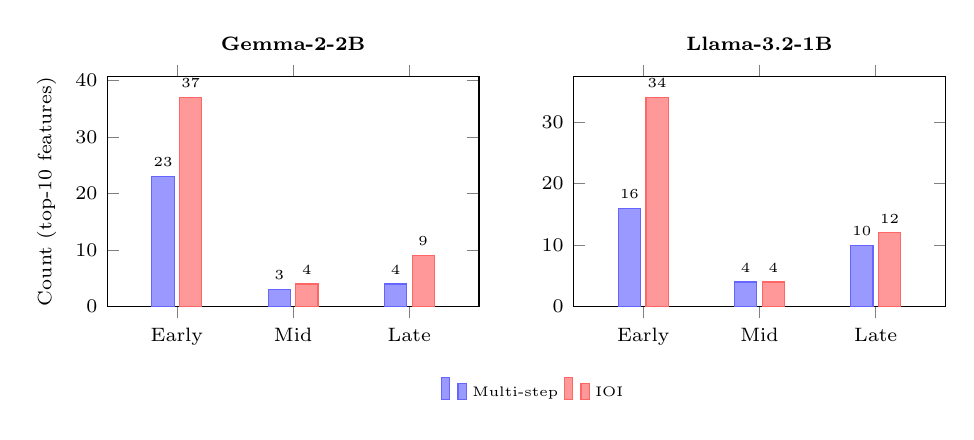
\begin{tikzpicture}
\begin{groupplot}[
    group style={
        group size=2 by 1,
        horizontal sep=1.2cm,
        ylabels at=edge left,
    },
    width=0.52\columnwidth,
    height=4.5cm,
    ylabel={Count (top-10 features)},
    symbolic x coords={Early, Mid, Late},
    xtick=data,
    x tick label style={font=\scriptsize},
    y tick label style={font=\scriptsize},
    ylabel style={font=\scriptsize},
    title style={font=\scriptsize\bfseries},
    ymin=0,
    enlarge x limits=0.3,
    nodes near coords,
    nodes near coords style={font=\tiny},
    legend image code/.code={\draw[#1] (0cm,-0.08cm) rectangle (0.30cm,0.12cm);},
    legend style={
        font=\tiny, draw=none,
        at={(1.15,-0.28)},
        anchor=north,
        legend columns=-1
    },
]

\nextgroupplot[ybar, bar width=8pt, title={Gemma-2-2B}]
\addplot[fill=blue!40, draw=blue!60] coordinates {
    (Early, 23) (Mid, 3) (Late, 4)
};

\addplot[fill=red!40, draw=red!60] coordinates {
    (Early, 37) (Mid, 4) (Late, 9)
};

\legend{Multi-step, IOI}

\nextgroupplot[ybar, bar width=8pt, title={Llama-3.2-1B}]
\addplot[fill=blue!40, draw=blue!60] coordinates {
    (Early, 16) (Mid, 4) (Late, 10)
};

\addplot[fill=red!40, draw=red!60] coordinates {
    (Early, 34) (Mid, 4) (Late, 12)
};

\end{groupplot}
\end{tikzpicture}
\DIFaddendFL 

\caption{Layer distribution of top-10 causal features for multi-step vs.\ IOI tasks on both models.}
\label{fig:layer_dist}
\end{figure}

The top causal features for multi-step prompts concentrate in early
layers (layers 0--8), consistent with the hypothesis that multi-hop
reasoning requires input processing and entity binding in lower layers
before final output computation.  This contrasts with IOI, where
late layers (24--25) dominate.


\subsection{Multi-Domain Analysis}

Table~\ref{tab:domain} presents per-domain \DIFdelbegin \DIFdel{results }\DIFdelend \DIFaddbegin \DIFadd{bounded oracle efficiency
}\DIFaddend across five cognitive categories\DIFdelbegin \DIFdel{.  Each domain is }\DIFdelend \DIFaddbegin \DIFadd{, each }\DIFaddend evaluated with two prompts
\DIFdelbegin \DIFdel{using }\DIFdelend \DIFaddbegin \DIFadd{under }\DIFaddend the same $B=20$ budget \DIFdelbegin \DIFdel{.  The bandit selector is now included for all domains.
}\DIFdelend \DIFaddbegin \DIFadd{and the fair ablation-only protocol.
}\DIFaddend 

\begin{table}[H]
\centering
\caption{\DIFdelbeginFL \DIFdelFL{Multi-Domain Feature Discovery}\DIFdelendFL \DIFaddbeginFL \DIFaddFL{Multi-domain bounded oracle efficiency (\%, ablation-only).
EAP and POMDP-abl vs.\ baselines.}\DIFaddendFL }
\label{tab:domain}
{\small
\DIFdelbeginFL %DIFDELCMD < \begin{tabular}{llcccc}
%DIFDELCMD < %%%
\DIFdelendFL \DIFaddbeginFL \begin{tabular}{llccccc}
\DIFaddendFL \toprule
\textbf{Model} & \textbf{Domain} & \textbf{\DIFdelbeginFL \DIFdelFL{POMDP KL}\DIFdelendFL \DIFaddbeginFL \DIFaddFL{EAP}\DIFaddendFL } & \textbf{\DIFdelbeginFL \DIFdelFL{Bandit KL}\DIFdelendFL \DIFaddbeginFL \DIFaddFL{POMDP-abl}\DIFaddendFL } & \textbf{\DIFdelbeginFL \DIFdelFL{vs.\ Rand.}\DIFdelendFL \DIFaddbeginFL \DIFaddFL{Bandit}\DIFaddendFL } & \textbf{\DIFdelbeginFL \DIFdelFL{vs.\ }\DIFdelendFL Greedy} \DIFaddbeginFL & \textbf{\DIFaddFL{Random}} \DIFaddendFL \\
\midrule
\multirow{5}{*}{Gemma}
 & Geography    & \DIFdelbeginFL \DIFdelFL{0.037   }\DIFdelendFL \DIFaddbeginFL \DIFaddFL{99.4 }\DIFaddendFL & \DIFdelbeginFL \DIFdelFL{0.003  }\DIFdelendFL \DIFaddbeginFL \DIFaddFL{94.0 }\DIFaddendFL & \DIFdelbeginFL \DIFdelFL{+1476\%  }\DIFdelendFL \DIFaddbeginFL \DIFaddFL{93.7 }\DIFaddendFL & \DIFdelbeginFL \DIFdelFL{+1324\% }\DIFdelendFL \DIFaddbeginFL \DIFaddFL{96.8 }& \DIFaddFL{40.9 }\DIFaddendFL \\
 & Mathematics  & \DIFdelbeginFL \DIFdelFL{0.035   }\DIFdelendFL \DIFaddbeginFL \DIFaddFL{99.7 }\DIFaddendFL & \DIFdelbeginFL \DIFdelFL{0.003  }\DIFdelendFL \DIFaddbeginFL \DIFaddFL{90.7 }\DIFaddendFL & \DIFdelbeginFL \DIFdelFL{+1267\%  }\DIFdelendFL \DIFaddbeginFL \DIFaddFL{96.4 }\DIFaddendFL & \DIFdelbeginFL \DIFdelFL{+1152\% }\DIFdelendFL \DIFaddbeginFL \DIFaddFL{18.6 }& \DIFaddFL{48.6 }\DIFaddendFL \\
 & Science      & \DIFdelbeginFL \DIFdelFL{0.026   }\DIFdelendFL \DIFaddbeginFL \DIFaddFL{89.5 }\DIFaddendFL & \DIFdelbeginFL \DIFdelFL{0.004  }\DIFdelendFL \DIFaddbeginFL \DIFaddFL{77.6 }\DIFaddendFL & \DIFdelbeginFL \DIFdelFL{+975\%   }\DIFdelendFL \DIFaddbeginFL \DIFaddFL{83.3 }\DIFaddendFL & \DIFdelbeginFL \DIFdelFL{+838\%  }\DIFdelendFL \DIFaddbeginFL \DIFaddFL{56.2 }& \DIFaddFL{57.4 }\DIFaddendFL \\
 & Logic        & \DIFdelbeginFL \DIFdelFL{0.051   }\DIFdelendFL \DIFaddbeginFL \DIFaddFL{97.5 }\DIFaddendFL & \DIFdelbeginFL \DIFdelFL{0.005  }\DIFdelendFL \DIFaddbeginFL \DIFaddFL{84.3 }\DIFaddendFL & \DIFdelbeginFL \DIFdelFL{+2125\%  }\DIFdelendFL \DIFaddbeginFL \DIFaddFL{54.8 }\DIFaddendFL & \DIFdelbeginFL \DIFdelFL{+1940\% }\DIFdelendFL \DIFaddbeginFL \DIFaddFL{89.1 }& \DIFaddFL{47.3 }\DIFaddendFL \\
 & History      & \DIFdelbeginFL \DIFdelFL{0.063   }\DIFdelendFL \DIFaddbeginFL \DIFaddFL{98.4 }\DIFaddendFL & \DIFdelbeginFL \DIFdelFL{0.005  }\DIFdelendFL \DIFaddbeginFL \DIFaddFL{90.4 }\DIFaddendFL & \DIFdelbeginFL \DIFdelFL{+2407\%  }\DIFdelendFL \DIFaddbeginFL \DIFaddFL{51.1 }\DIFaddendFL & \DIFdelbeginFL \DIFdelFL{+2312\% }\DIFdelendFL \DIFaddbeginFL \DIFaddFL{71.8 }& \DIFaddFL{58.8 }\DIFaddendFL \\
\midrule
\multirow{5}{*}{Llama}
 & Geography    & \DIFdelbeginFL \DIFdelFL{0.040   }\DIFdelendFL \DIFaddbeginFL \DIFaddFL{95.2 }\DIFaddendFL & \DIFdelbeginFL \DIFdelFL{0.019  }\DIFdelendFL \DIFaddbeginFL \DIFaddFL{97.6 }\DIFaddendFL & \DIFdelbeginFL \DIFdelFL{+203\%   }\DIFdelendFL \DIFaddbeginFL \DIFaddFL{93.3 }\DIFaddendFL & \DIFdelbeginFL \DIFdelFL{$-$32.4\%  }\DIFdelendFL \DIFaddbeginFL \DIFaddFL{96.5 }& \DIFaddFL{51.1 }\DIFaddendFL \\
 & Mathematics  & \DIFdelbeginFL \DIFdelFL{0.053   }\DIFdelendFL \DIFaddbeginFL \DIFaddFL{98.3 }\DIFaddendFL & \DIFdelbeginFL \DIFdelFL{0.015  }\DIFdelendFL \DIFaddbeginFL \DIFaddFL{90.5 }\DIFaddendFL & \DIFdelbeginFL \DIFdelFL{+300\%   }\DIFdelendFL \DIFaddbeginFL \DIFaddFL{87.4 }\DIFaddendFL & \DIFdelbeginFL \DIFdelFL{$-$3.7\%   }\DIFdelendFL \DIFaddbeginFL \DIFaddFL{90.6 }& \DIFaddFL{49.8 }\DIFaddendFL \\
 & Science      & \DIFdelbeginFL \DIFdelFL{0.002   }\DIFdelendFL \DIFaddbeginFL \DIFaddFL{82.4 }\DIFaddendFL & \DIFdelbeginFL \DIFdelFL{0.003  }\DIFdelendFL \DIFaddbeginFL \DIFaddFL{88.2 }\DIFaddendFL & \DIFdelbeginFL \DIFdelFL{$-$22\%  }\DIFdelendFL \DIFaddbeginFL \DIFaddFL{67.9 }\DIFaddendFL & \DIFdelbeginFL \DIFdelFL{$-$9.5\%   }\DIFdelendFL \DIFaddbeginFL \DIFaddFL{55.5 }& \DIFaddFL{42.7 }\DIFaddendFL \\
 & Logic        & \DIFdelbeginFL \DIFdelFL{0.463   }\DIFdelendFL \DIFaddbeginFL \DIFaddFL{77.2 }\DIFaddendFL & \DIFdelbeginFL \DIFdelFL{0.045  }\DIFdelendFL \DIFaddbeginFL \DIFaddFL{66.2 }\DIFaddendFL & \DIFdelbeginFL \DIFdelFL{+3000\%  }\DIFdelendFL \DIFaddbeginFL \DIFaddFL{41.3 }\DIFaddendFL & \DIFdelbeginFL \DIFdelFL{+1500\%    }\DIFdelendFL \DIFaddbeginFL \DIFaddFL{67.4 }& \DIFaddFL{53.8 }\DIFaddendFL \\
 & History      & \DIFdelbeginFL \DIFdelFL{0.357   }\DIFdelendFL \DIFaddbeginFL \DIFaddFL{97.9 }\DIFaddendFL & \DIFdelbeginFL \DIFdelFL{0.037  }\DIFdelendFL \DIFaddbeginFL \DIFaddFL{56.7 }\DIFaddendFL & \DIFdelbeginFL \DIFdelFL{+2600\%  }\DIFdelendFL \DIFaddbeginFL \DIFaddFL{55.1 }\DIFaddendFL & \DIFdelbeginFL \DIFdelFL{+1390\%    }\DIFdelendFL \DIFaddbeginFL \DIFaddFL{26.4 }& \DIFaddFL{37.6 }\DIFaddendFL \\
\bottomrule
\end{tabular}%
}
\end{table}

\DIFdelbegin \DIFdel{The POMDP agent substantially outperforms all baselines on most
domains on
both models .  Gemmashows consistently strong performance
across all five domains.  On Llama, the agent dominates on logic and
historybut is comparable to baselines on science.
}\DIFdelend \DIFaddbegin \DIFadd{Under the fair protocol POMDP-abl is a solid selector across domains on
}\emph{\DIFadd{both}} \DIFadd{models (77--94\% on Gemma, 57--98\% on Llama): it beats
random in every domain and is competitive with the bandit and greedy,
winning on some domains (e.g.\ Gemma logic/history, Llama science/logic)
and trailing on others (e.g.\ Gemma math/science).  EAP remains the
strongest single baseline.  The domain results thus mirror the IOI
picture: the agent reliably beats random and is competitive with
greedy/bandit, while EAP attribution ranking is hard to beat.  (Absolute multi-action KL per domain is
steering-amplified and reported as RCK context, not as oracle
efficiency.)
}\DIFaddend 

The corresponding per-domain layer distributions are shown in
Figure~\ref{fig:domain_layers}, which makes the task-dependent
structure explicit: reasoning domains are left-heavy (early layers)
while factual domains are right-heavy (late layers) on both models.

\begin{figure}[H]
\centering
% Auto-generated from experiment results.
\DIFdelbeginFL %DIFDELCMD < \begin{tikzpicture}
%DIFDELCMD < \begin{groupplot}[
%DIFDELCMD <     group style={
%DIFDELCMD <         group size=2 by 1,
%DIFDELCMD <         horizontal sep=0.5cm,
%DIFDELCMD <         ylabels at=edge left,
%DIFDELCMD <     },
%DIFDELCMD <     width=0.48\linewidth,
%DIFDELCMD <     height=6cm,
%DIFDELCMD <     ylabel={Count (top-10 features)},
%DIFDELCMD <     symbolic x coords={Geo., Math, Sci., Logic, Hist.},
%DIFDELCMD <     xtick=data,
%DIFDELCMD <     x tick label style={font=\scriptsize},
%DIFDELCMD <     y tick label style={font=\scriptsize},
%DIFDELCMD <     ylabel style={font=\scriptsize},
%DIFDELCMD <     title style={font=\scriptsize\bfseries},
%DIFDELCMD <     ymin=0,
%DIFDELCMD <     enlarge x limits=0.15,
%DIFDELCMD <     nodes near coords,
%DIFDELCMD <     nodes near coords style={font=\tiny, anchor=north},
%DIFDELCMD <     legend style={
%DIFDELCMD <         font=\tiny,
%DIFDELCMD <         at={(0.5,-0.38)},
%DIFDELCMD <         anchor=north,
%DIFDELCMD <         legend columns=3
%DIFDELCMD <     },
%DIFDELCMD <     ymajorgrids=true,
%DIFDELCMD <     grid style={dashed, gray!30},
%DIFDELCMD < ]
%DIFDELCMD < 

%DIFDELCMD < \nextgroupplot[ybar, bar width=4pt, title={Gemma-2-2B}]
%DIFDELCMD < \addplot[fill=blue!50, draw=blue!70] coordinates { (Geo., 14) (Math, 0) (Sci., 11) (Logic, 14) (Hist., 15) };
%DIFDELCMD < \addplot[fill=green!40, draw=green!60] coordinates { (Geo., 0) (Math, 0) (Sci., 3) (Logic, 1) (Hist., 2) };
%DIFDELCMD < \addplot[fill=red!40, draw=red!60] coordinates { (Geo., 6) (Math, 0) (Sci., 6) (Logic, 5) (Hist., 3) };
%DIFDELCMD < \legend{Early, Mid, Late}
%DIFDELCMD < 

%DIFDELCMD < \nextgroupplot[ybar, bar width=4pt, title={Llama-3.2-1B}]
%DIFDELCMD < \addplot[fill=blue!50, draw=blue!70] coordinates { (Geo., 7) (Math, 0) (Sci., 12) (Logic, 15) (Hist., 14) };
%DIFDELCMD < \addplot[fill=green!40, draw=green!60] coordinates { (Geo., 3) (Math, 0) (Sci., 2) (Logic, 3) (Hist., 4) };
%DIFDELCMD < \addplot[fill=red!40, draw=red!60] coordinates { (Geo., 10) (Math, 0) (Sci., 6) (Logic, 2) (Hist., 2) };
%DIFDELCMD < 

%DIFDELCMD < \end{groupplot}
%DIFDELCMD < \end{tikzpicture}
%DIFDELCMD < %%%
\DIFdelendFL \DIFaddbeginFL 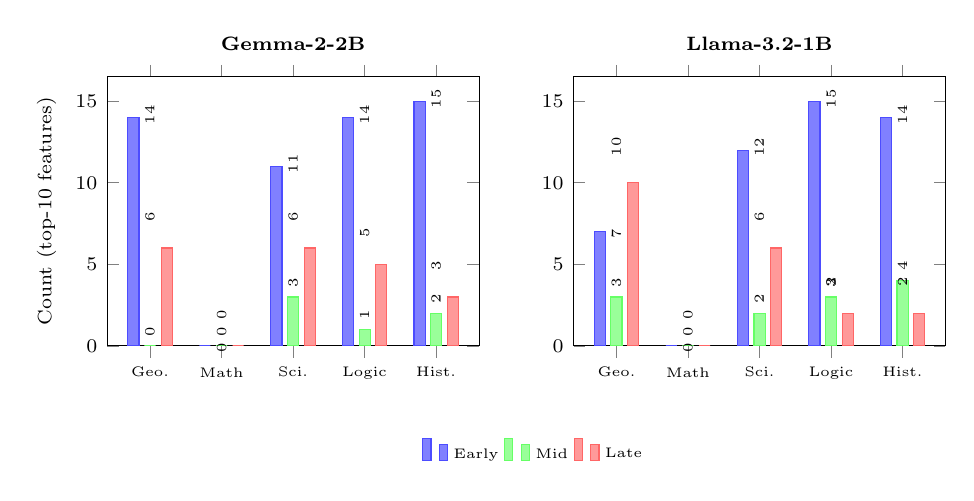
\begin{tikzpicture}
\begin{groupplot}[
    group style={
        group size=2 by 1,
        horizontal sep=1.2cm,
        ylabels at=edge left,
    },
    width=0.52\columnwidth,
    height=5cm,
    ylabel={Count (top-10 features)},
    symbolic x coords={Geo., Math, Sci., Logic, Hist.},
    xtick=data,
    x tick label style={font=\tiny},
    y tick label style={font=\scriptsize},
    ylabel style={font=\scriptsize},
    title style={font=\scriptsize\bfseries},
    ymin=0,
    enlarge x limits=0.15,
    nodes near coords,
    nodes near coords style={font=\tiny, rotate=90, anchor=west},
    legend image code/.code={\draw[#1] (0cm,-0.08cm) rectangle (0.30cm,0.12cm);},
    legend style={
        font=\tiny, draw=none,
        at={(1.15,-0.32)},
        anchor=north,
        legend columns=-1
    },
]

\nextgroupplot[ybar, bar width=4pt, title={Gemma-2-2B}]
\addplot[fill=blue!50, draw=blue!70] coordinates { (Geo., 14) (Math, 0) (Sci., 11) (Logic, 14) (Hist., 15) };
\addplot[fill=green!40, draw=green!60] coordinates { (Geo., 0) (Math, 0) (Sci., 3) (Logic, 1) (Hist., 2) };
\addplot[fill=red!40, draw=red!60] coordinates { (Geo., 6) (Math, 0) (Sci., 6) (Logic, 5) (Hist., 3) };
\legend{Early, Mid, Late}

\nextgroupplot[ybar, bar width=4pt, title={Llama-3.2-1B}]
\addplot[fill=blue!50, draw=blue!70] coordinates { (Geo., 7) (Math, 0) (Sci., 12) (Logic, 15) (Hist., 14) };
\addplot[fill=green!40, draw=green!60] coordinates { (Geo., 3) (Math, 0) (Sci., 2) (Logic, 3) (Hist., 4) };
\addplot[fill=red!40, draw=red!60] coordinates { (Geo., 10) (Math, 0) (Sci., 6) (Logic, 2) (Hist., 2) };

\end{groupplot}
\end{tikzpicture}
\DIFaddendFL 

\caption{Layer distribution of top-10 causal features across five cognitive domains on both models.}
\label{fig:domain_layers}
\end{figure}

The multi-domain analysis reveals task-dependent circuit structure:
reasoning tasks (logic, mathematics) recruit early-layer features,
while factual tasks (geography, history) concentrate in late layers.
Science prompts show \DIFaddbegin \DIFadd{a }\DIFaddend more uniform distribution.


\subsection{\DIFdelbegin \DIFdel{Cross-Model Validation (Llama-3.2-1B)}\DIFdelend \DIFaddbegin \DIFadd{Discretisation Sensitivity}\DIFaddend }
\DIFaddbegin \label{sec:sensitivity}
\DIFaddend 

\DIFdelbegin \DIFdel{To validate generality, all experiments are replicated on
Llama-3.2-1B (16 layers, 2048-dim)using transcoders from
}\texttt{\DIFdel{mntss/transcoder-Llama-3.2-1B}}%DIFAUXCMD
\DIFdel{.
The side-by-side comparison
of mean KL and oracle efficiency across both architectures is given in
Table~\ref{tab:crossmodel}}\DIFdelend \DIFaddbegin \DIFadd{The observation model discretises continuous KL and activation
magnitudes into bins via fixed thresholds (Section~\ref{sec:setup})}\DIFaddend .
\DIFaddbegin \DIFadd{To check that conclusions are not artefacts of these thresholds, Gemma
IOI was re-run with the KL and activation thresholds independently
scaled by $\pm 20\%$ and POMDP-abl bounded oracle
efficiency recomputed (Table~\ref{tab:sensitivity}).
}\DIFaddend 

\begin{table}[H]
\centering
\caption{\DIFdelbeginFL \DIFdelFL{Cross-Model Comparison}\DIFdelendFL \DIFaddbeginFL \DIFaddFL{Discretisation sensitivity}\DIFaddendFL : \DIFdelbeginFL \DIFdelFL{Gemma-2-2B vs}\DIFdelendFL \DIFaddbeginFL \DIFaddFL{Gemma IOI POMDP-abl bounded
oracle efficiency under $\pm 20\%$ threshold perturbations
(baseline 82.0\%)}\DIFaddendFL .\DIFdelbeginFL \DIFdelFL{\ Llama-3.2-1B}\DIFdelendFL }
\DIFdelbeginFL %DIFDELCMD < \label{tab:crossmodel}
%DIFDELCMD < %%%
\DIFdelendFL \DIFaddbeginFL \label{tab:sensitivity}
\DIFaddendFL {\small
\DIFdelbeginFL %DIFDELCMD < \begin{tabular}{lllcc}
%DIFDELCMD < %%%
\DIFdelendFL \DIFaddbeginFL \begin{tabular}{lc}
\DIFaddendFL \toprule
\textbf{\DIFdelbeginFL \DIFdelFL{Model}\DIFdelendFL \DIFaddbeginFL \DIFaddFL{Perturbation}\DIFaddendFL } & \textbf{\DIFdelbeginFL \DIFdelFL{Task}\DIFdelendFL \DIFaddbeginFL \DIFaddFL{Oracle Eff.\ (\%)}\DIFaddendFL } \DIFdelbeginFL %DIFDELCMD < & %%%
\textbf{\DIFdelFL{Method}} %DIFAUXCMD
%DIFDELCMD < & %%%
\textbf{\DIFdelFL{Mean KL}} %DIFAUXCMD
%DIFDELCMD < & %%%
\textbf{\DIFdelFL{Oracle Eff.}} %DIFAUXCMD
\DIFdelendFL \\
\midrule
\DIFdelbeginFL %DIFDELCMD < \multirow{4}{*}{Gemma-2-2B}
%DIFDELCMD <  %%%
\DIFdelendFL \DIFaddbeginFL \DIFaddFL{Baseline thresholds            }\DIFaddendFL & \DIFdelbeginFL \DIFdelFL{IOI        }\DIFdelendFL \DIFaddbeginFL \DIFaddFL{82.0 }\\
\DIFaddFL{Activation thresholds $\times 0.8$ }\DIFaddendFL & \DIFdelbeginFL \DIFdelFL{POMDP Agent }\DIFdelendFL \DIFaddbeginFL \DIFaddFL{86.2 }\\
\DIFaddFL{Activation thresholds $\times 1.2$ }\DIFaddendFL & \DIFdelbeginFL \DIFdelFL{0.010824 }\DIFdelendFL \DIFaddbeginFL \DIFaddFL{80.3 }\\
\DIFaddFL{KL thresholds $\times 1.2$         }\DIFaddendFL & \DIFdelbeginFL \DIFdelFL{1255.0\% }\DIFdelendFL \DIFaddbeginFL \DIFaddFL{82.0 }\DIFaddendFL \\
\DIFaddbeginFL \DIFaddFL{KL thresholds $\times 0.8$         }\DIFaddendFL & \DIFdelbeginFL \DIFdelFL{IOI        }\DIFdelendFL \DIFaddbeginFL \DIFaddFL{60.2 }\\
\bottomrule
\end{tabular}%DIF > 
}
\end{table}

\DIFadd{Efficiency is stable (80--86\%) under activation-threshold changes and
under a $+20\%$ KL-threshold change, but drops to 60.2\% when the KL
thresholds are tightened by $20\%$.  The KL discretisation is thus the
more sensitive knob: overly fine KL bins inject observation noise into
the belief update.  The qualitative ordering (POMDP-abl above random,
competitive with the bandit, below EAP) is preserved in all five
configurations, so the headline conclusions are robust to reasonable
threshold choices while the precise efficiency value is not.
}

\DIFadd{A complementary sweep over the agent's three core hyperparameters, the
action precision $\gamma$, the Dirichlet likelihood learning rate $\eta$,
and the pragmatic preference weight, confirms that the bounded oracle
efficiency is highly stable to these settings
(Table~\ref{tab:hpsensitivity}).  On Gemma IOI the efficiency stays at
$82.0\%$ across a sixteen-fold range of $\gamma$, a four-fold range of
$\eta$, and a four-fold range of the pragmatic weight.  On Llama IOI it
is invariant to $\gamma$ and the pragmatic weight, and varies only
mildly with $\eta$ (49.1--54.5\%).  The agent's behaviour is therefore
governed by the structure of its generative model and the observation
stream rather than by fine hyperparameter tuning.
}

\begin{table}[H]
\centering
\caption{\DIFaddFL{Hyperparameter sensitivity of POMDP-abl bounded oracle
efficiency (\%) on IOI, varying one factor at a time about the default
($\gamma{=}16$, $\eta{=}1.0$, pragmatic weight $1.0$).}}
\label{tab:hpsensitivity}
{\small
\begin{tabular}{llcc}
\toprule
\textbf{\DIFaddFL{Factor}} \DIFaddendFL & \DIFdelbeginFL \DIFdelFL{Bandit      }\DIFdelendFL \DIFaddbeginFL \textbf{\DIFaddFL{Value}} \DIFaddendFL & \DIFdelbeginFL \DIFdelFL{0.000642 }\DIFdelendFL \DIFaddbeginFL \textbf{\DIFaddFL{Gemma-2-2B}} \DIFaddendFL & \DIFdelbeginFL \DIFdelFL{74.4\% }\DIFdelendFL \DIFaddbeginFL \textbf{\DIFaddFL{Llama-3.2-1B}} \DIFaddendFL \\
\DIFaddbeginFL \midrule
\DIFaddFL{Action precision $\gamma$ }\DIFaddendFL & \DIFdelbeginFL \DIFdelFL{Multi-step }\DIFdelendFL \DIFaddbeginFL \DIFaddFL{4   }\DIFaddendFL & \DIFdelbeginFL \DIFdelFL{POMDP Agent }\DIFdelendFL \DIFaddbeginFL \DIFaddFL{82.0 }\DIFaddendFL & \DIFdelbeginFL \DIFdelFL{0.004965 }%DIFDELCMD < & %%%
\DIFdelFL{983.0\% }\DIFdelendFL \DIFaddbeginFL \DIFaddFL{52.1 }\DIFaddendFL \\
                          & \DIFdelbeginFL \DIFdelFL{Multi-step }\DIFdelendFL \DIFaddbeginFL \DIFaddFL{64  }\DIFaddendFL & \DIFdelbeginFL \DIFdelFL{Bandit      }\DIFdelendFL \DIFaddbeginFL \DIFaddFL{82.0 }\DIFaddendFL & \DIFdelbeginFL \DIFdelFL{0.000396 }%DIFDELCMD < & %%%
\DIFdelFL{78.4\% }\DIFdelendFL \DIFaddbeginFL \DIFaddFL{52.1 }\DIFaddendFL \\
\midrule
\DIFdelbeginFL %DIFDELCMD < \multirow{4}{*}{Llama-3.2-1B}
%DIFDELCMD <  %%%
\DIFdelendFL \DIFaddbeginFL \DIFaddFL{Learning rate $\eta$      }\DIFaddendFL & \DIFdelbeginFL \DIFdelFL{IOI        }\DIFdelendFL \DIFaddbeginFL \DIFaddFL{0.5 }\DIFaddendFL & \DIFdelbeginFL \DIFdelFL{POMDP Agent }\DIFdelendFL \DIFaddbeginFL \DIFaddFL{82.0 }\DIFaddendFL & \DIFdelbeginFL \DIFdelFL{0.008833 }%DIFDELCMD < & %%%
\DIFdelFL{90.6\% }\DIFdelendFL \DIFaddbeginFL \DIFaddFL{54.5 }\DIFaddendFL \\
                          & \DIFdelbeginFL \DIFdelFL{IOI        }\DIFdelendFL \DIFaddbeginFL \DIFaddFL{2.0 }\DIFaddendFL & \DIFdelbeginFL \DIFdelFL{Bandit      }\DIFdelendFL \DIFaddbeginFL \DIFaddFL{82.0 }\DIFaddendFL & \DIFdelbeginFL \DIFdelFL{0.008606 }%DIFDELCMD < & %%%
\DIFdelFL{88.2\% }\DIFdelendFL \DIFaddbeginFL \DIFaddFL{49.1 }\DIFaddendFL \\
\DIFaddbeginFL \midrule
\DIFaddFL{Pragmatic weight          }\DIFaddendFL & \DIFdelbeginFL \DIFdelFL{Multi-step }\DIFdelendFL \DIFaddbeginFL \DIFaddFL{0.5 }\DIFaddendFL & \DIFdelbeginFL \DIFdelFL{POMDP Agent }\DIFdelendFL \DIFaddbeginFL \DIFaddFL{81.9 }\DIFaddendFL & \DIFdelbeginFL \DIFdelFL{0.004110 }%DIFDELCMD < & %%%
\DIFdelFL{33.6\%  }\DIFdelendFL \DIFaddbeginFL \DIFaddFL{52.1 }\DIFaddendFL \\
                          & \DIFdelbeginFL \DIFdelFL{Multi-step }\DIFdelendFL \DIFaddbeginFL \DIFaddFL{2.0 }\DIFaddendFL & \DIFdelbeginFL \DIFdelFL{Bandit      }\DIFdelendFL \DIFaddbeginFL \DIFaddFL{82.0 }\DIFaddendFL & \DIFdelbeginFL \DIFdelFL{0.009352 }%DIFDELCMD < & %%%
\DIFdelFL{76.4\% }\DIFdelendFL \DIFaddbeginFL \DIFaddFL{52.1 }\DIFaddendFL \\
\bottomrule
\end{tabular}%
}
\end{table}


\DIFdelbegin \DIFdel{The budget is $B=20$ on all experiments .  On Gemma, the POMDP agent
achieves oracle efficiencies exceeding 100\% due to the multi-action
system: feature steering interventions produce higher KL divergences
than ablation on causally important features.  On Llama, the POMDP
agent outperforms the bandit on IOI (90.6\% vs.\ 88.2\%) but trails
on multi-step (33.6\% vs.  \ 76.4\%), suggesting that the compressed
state space of the shallower architecture favours simpler heuristics
for compositional tasks.
}\DIFdelend \DIFaddbegin \subsection{\DIFadd{Cross-Model Validation (Llama-3.2-1B)}}
\DIFaddend 

\DIFdelbegin \subsection{\DIFdel{Efficiency Comparison}}
%DIFAUXCMD
\addtocounter{subsection}{-1}%DIFAUXCMD
%DIFDELCMD < 

%DIFDELCMD < %%%
\DIFdel{Relative efficiency gains of the POMDP agent over the random baseline
}\DIFdelend \DIFaddbegin \DIFadd{To probe generality, all experiments are replicated on Llama-3.2-1B
(16 layers, 2048-dim) using transcoders from
}\texttt{\DIFadd{mntss/transcoder-Llama-3.2-1B}}\DIFadd{.  Table~\ref{tab:crossmodel}
provides a consolidated head-to-head of the four ablation-only
selectors against the EAP and ablation oracles }\DIFaddend across all three \DIFdelbegin \DIFdel{benchmark families are summarised in
Table~\ref{tab:efficiency}}\DIFdelend \DIFaddbegin \DIFadd{task
families and both architectures}\DIFaddend .

\begin{table}[H]
\centering
\caption{\DIFdelbeginFL \DIFdelFL{Efficiency Improvement Over Baselines}\DIFdelendFL \DIFaddbeginFL \DIFaddFL{Head-to-head bounded oracle efficiency (\%, ablation-only)
across IOI, multi-step, and domain tasks for both models. Domain values
are means over the five cognitive domains.}\DIFaddendFL }
\DIFdelbeginFL %DIFDELCMD < \label{tab:efficiency}
%DIFDELCMD < %%%
\DIFdelendFL \DIFaddbeginFL \label{tab:crossmodel}
\DIFaddendFL {\small
\DIFdelbeginFL %DIFDELCMD < \begin{tabular}{lllcc}
%DIFDELCMD < %%%
\DIFdelendFL \DIFaddbeginFL \begin{tabular}{llcc}
\DIFaddendFL \toprule
\DIFdelbeginFL \textbf{\DIFdelFL{Model}} %DIFAUXCMD
%DIFDELCMD < & %%%
\DIFdelendFL \textbf{Task} & \textbf{\DIFdelbeginFL \DIFdelFL{Comparison}\DIFdelendFL \DIFaddbeginFL \DIFaddFL{Method}\DIFaddendFL } & \textbf{\DIFdelbeginFL \DIFdelFL{Improv.}\DIFdelendFL \DIFaddbeginFL \DIFaddFL{Gemma-2-2B}\DIFaddendFL } & \textbf{\DIFdelbeginFL \DIFdelFL{Oracle Eff.}\DIFdelendFL \DIFaddbeginFL \DIFaddFL{Llama-3.2-1B}\DIFaddendFL } \\
\midrule
\DIFdelbeginFL %DIFDELCMD < \multirow{3}{*}{Gemma}
%DIFDELCMD <  %%%
\DIFdelendFL \DIFaddbeginFL \multirow{4}{*}{IOI}
 \DIFaddendFL & \DIFdelbeginFL \DIFdelFL{IOI        }\DIFdelendFL \DIFaddbeginFL \DIFaddFL{EAP       }\DIFaddendFL & \DIFdelbeginFL \DIFdelFL{POMDP vs.\ Random }\DIFdelendFL \DIFaddbeginFL \DIFaddFL{91.9 }\DIFaddendFL & \DIFdelbeginFL \DIFdelFL{+2336\%   }\DIFdelendFL \DIFaddbeginFL \DIFaddFL{95.2 }\\
 \DIFaddendFL & \DIFdelbeginFL \DIFdelFL{1255.0\%  }\DIFdelendFL \DIFaddbeginFL \DIFaddFL{POMDP-abl }& \DIFaddFL{82.0 }& \DIFaddFL{52.1 }\DIFaddendFL \\
 & \DIFdelbeginFL \DIFdelFL{Multi-step }\DIFdelendFL \DIFaddbeginFL \DIFaddFL{Bandit    }\DIFaddendFL & \DIFdelbeginFL \DIFdelFL{POMDP vs.\ Random }\DIFdelendFL \DIFaddbeginFL \DIFaddFL{74.4 }\DIFaddendFL & \DIFdelbeginFL \DIFdelFL{+1756\%   }\DIFdelendFL \DIFaddbeginFL \DIFaddFL{88.2 }\\
 \DIFaddendFL & \DIFdelbeginFL \DIFdelFL{983.0\%   }\DIFdelendFL \DIFaddbeginFL \DIFaddFL{UCB       }& \DIFaddFL{73.7 }& \DIFaddFL{55.2 }\DIFaddendFL \\
\DIFaddbeginFL \midrule
\multirow{4}{*}{Multi-step}
 \DIFaddendFL & \DIFdelbeginFL \DIFdelFL{Domain     }\DIFdelendFL \DIFaddbeginFL \DIFaddFL{EAP       }\DIFaddendFL & \DIFdelbeginFL \DIFdelFL{POMDP vs.\ Random }\DIFdelendFL \DIFaddbeginFL \DIFaddFL{98.1 }\DIFaddendFL & \DIFdelbeginFL \DIFdelFL{+1482\%   }\DIFdelendFL \DIFaddbeginFL \DIFaddFL{97.6 }\\
 \DIFaddendFL & \DIFdelbeginFL \DIFdelFL{---       }\DIFdelendFL \DIFaddbeginFL \DIFaddFL{POMDP-abl }& \DIFaddFL{73.0 }& \phantom{0}\DIFaddFL{9.3 }\DIFaddendFL \\
 \DIFdelbeginFL %DIFDELCMD < \midrule
%DIFDELCMD < \multirow{3}{*}{Llama}
%DIFDELCMD <  %%%
\DIFdelendFL & \DIFdelbeginFL \DIFdelFL{IOI        }\DIFdelendFL \DIFaddbeginFL \DIFaddFL{Bandit    }\DIFaddendFL & \DIFdelbeginFL \DIFdelFL{POMDP vs.\ Random }\DIFdelendFL \DIFaddbeginFL \DIFaddFL{78.4 }\DIFaddendFL & \DIFdelbeginFL \DIFdelFL{+143.9\%  }\DIFdelendFL \DIFaddbeginFL \DIFaddFL{76.4 }\\
 \DIFaddendFL & \DIFdelbeginFL \DIFdelFL{90.6\%    }\DIFdelendFL \DIFaddbeginFL \DIFaddFL{UCB       }& \DIFaddFL{73.6 }& \DIFaddFL{75.9 }\DIFaddendFL \\
\DIFaddbeginFL \midrule
\multirow{4}{*}{Domain}
 \DIFaddendFL & \DIFdelbeginFL \DIFdelFL{Multi-step }\DIFdelendFL \DIFaddbeginFL \DIFaddFL{EAP       }\DIFaddendFL & \DIFdelbeginFL \DIFdelFL{POMDP vs.\ Random }\DIFdelendFL \DIFaddbeginFL \DIFaddFL{96.9 }\DIFaddendFL & \DIFdelbeginFL \DIFdelFL{$-$34.9\% }\DIFdelendFL \DIFaddbeginFL \DIFaddFL{90.2 }\\
 \DIFaddendFL & \DIFdelbeginFL \DIFdelFL{33.6\%    }\DIFdelendFL \DIFaddbeginFL \DIFaddFL{POMDP-abl }& \DIFaddFL{87.4 }& \DIFaddFL{79.9 }\DIFaddendFL \\
 & \DIFdelbeginFL \DIFdelFL{Domain     }\DIFdelendFL \DIFaddbeginFL \DIFaddFL{Bandit    }\DIFaddendFL & \DIFdelbeginFL \DIFdelFL{POMDP vs.\ Random }\DIFdelendFL \DIFaddbeginFL \DIFaddFL{75.9 }\DIFaddendFL & \DIFdelbeginFL \DIFdelFL{+1137\%   }\DIFdelendFL \DIFaddbeginFL \DIFaddFL{69.0 }\\
 \DIFaddendFL & \DIFdelbeginFL \DIFdelFL{---       }\DIFdelendFL \DIFaddbeginFL \DIFaddFL{UCB       }& \DIFaddFL{77.1 }& \DIFaddFL{66.7 }\DIFaddendFL \\
\bottomrule
\end{tabular}%
}
\end{table}

The \DIFdelbegin \DIFdel{POMDP agent substantially outperforms randomselection on both architectures for IOI and }\DIFdelend \DIFaddbegin \DIFadd{agent transfers cleanly to Gemma's deeper stack, where POMDP-abl
beats random, edges out both the heuristic bandit and plain UCB, and is
the strongest non-EAP selector across IOI and the }\DIFaddend domain tasks.  On
\DIFdelbegin \DIFdel{Gemma, improvements
exceed 1482\%across all benchmarks, driven by the agent's ability
to select both feature and intervention type via EFE minimisation}\DIFdelend \DIFaddbegin \DIFadd{Llama it transfers only partially: it remains competitive on the
single-step domain tasks (79.9\%, above both bandit and UCB), but on
IOI its efficiency (52.1\%) is only marginally above random (48.4\%)
and well below the bandit (88.2\%) and EAP (95.2\%), and the coarse
layer-role discretisation hurts it badly on multi-step reasoning
(Section~\ref{sec:multistep}).  The heuristic
bandit and the plain UCB baseline track each other closely on Gemma
(both near 74--78\%), indicating that the bandit's hand-built importance
and locality priors add little there}\DIFaddend . On Llama \DIFdelbegin \DIFdel{, the agent outperforms random on IOI and domain tasks but under-performs on multi-step reasoning}\DIFdelend \DIFaddbegin \DIFadd{IOI, by contrast, the heuristic
bandit (88.2\%) far exceeds plain UCB (55.2\%), showing that those priors
carry the bandit on the shallower architecture.  Overall the agent is
competitive with, and often slightly ahead of, the action-matched
baselines on Gemma, but behind the heuristic bandit on the shallower
Llama stack}\DIFaddend .


\subsection{Hypothesis Evaluation}

The four pre-registered hypotheses (H1--H4) are evaluated against the
experimental evidence and summarised in
Table~\ref{tab:hypothesis_eval}.  \DIFaddbegin \DIFadd{H2 is split into manipulability
(H2a) and selectivity (H2b) following the steering controls above.
}\DIFaddend 

\begin{table}[H]
\centering
\caption{Hypothesis \DIFdelbeginFL \DIFdelFL{Evaluation Summary}\DIFdelendFL \DIFaddbeginFL \DIFaddFL{evaluation summary.  H1/H3 shown as Gemma / Llama.}\DIFaddendFL }
\label{tab:hypothesis_eval}
{\footnotesize
\DIFdelbeginFL %DIFDELCMD < \begin{tabular}{lcccc}
%DIFDELCMD < %%%
\DIFdelendFL \DIFaddbeginFL \begin{tabular}{p{2.0cm}p{3.4cm}p{2.6cm}p{1.8cm}p{2.4cm}}
\DIFaddendFL \toprule
\textbf{Hypothesis} & \textbf{Criterion} & \textbf{Result} & \textbf{$p$-value} & \textbf{Outcome} \\
\midrule
H1: Efficiency  & \DIFdelbeginFL \DIFdelFL{POMDP }\DIFdelendFL \DIFaddbeginFL \DIFaddFL{POMDP-abl }\DIFaddendFL $>$ Random (paired \DIFdelbeginFL \DIFdelFL{$t$}\DIFdelendFL \DIFaddbeginFL \DIFaddFL{perm.}\DIFaddendFL ) & \DIFdelbeginFL \DIFdelFL{+2336\% / +143.9\% }\DIFdelendFL \DIFaddbeginFL \DIFaddFL{$+43.5\%$ / $+7.8\%$ }\DIFaddendFL & \DIFdelbeginFL \DIFdelFL{0.01 / 0.12  }\DIFdelendFL \DIFaddbeginFL \DIFaddFL{0.031 / 0.41 }\DIFaddendFL & \DIFdelbeginFL \textbf{\DIFdelFL{Accepted (Gemma)}}  %DIFAUXCMD
\DIFdelendFL \DIFaddbeginFL \DIFaddFL{Accepted (Gemma); not on Llama }\DIFaddendFL \\
\DIFdelbeginFL \DIFdelFL{H2: Causal ctrl}\DIFdelendFL \DIFaddbeginFL \DIFaddFL{H2a: Manipulab}\DIFaddendFL . & \DIFdelbeginFL \DIFdelFL{Binomial }\DIFdelendFL \DIFaddbeginFL \DIFaddFL{Steering changes }\DIFaddendFL $>$ \DIFdelbeginFL \DIFdelFL{1\%             }\DIFdelendFL \DIFaddbeginFL \DIFaddFL{chance }\DIFaddendFL & \DIFdelbeginFL \DIFdelFL{24/200               }\DIFdelendFL \DIFaddbeginFL \DIFaddFL{11/50 \& 9/50 at $m{=}10$ }\DIFaddendFL & \DIFdelbeginFL \DIFdelFL{$<$0.001     }\DIFdelendFL \DIFaddbeginFL \DIFaddFL{$<10^{-8}$ }\DIFaddendFL & \DIFdelbeginFL \textbf{\DIFdelFL{Accepted}}  %DIFAUXCMD
\DIFdelendFL \DIFaddbeginFL \DIFaddFL{Accepted }\DIFaddendFL \\
\DIFaddbeginFL \DIFaddFL{H2b: Selectivity }& \DIFaddFL{Selected $>$ control (Fisher) }& \DIFaddFL{11 vs 8; 9 vs 6 }& \DIFaddFL{n.s. }& \DIFaddFL{Not supported }\\
\DIFaddendFL H3: Discovery    & \DIFdelbeginFL \DIFdelFL{Oracle }\DIFdelendFL \DIFaddbeginFL \DIFaddFL{Bounded oracle }\DIFaddendFL eff.\ $\geq 50\%$ & \DIFdelbeginFL \DIFdelFL{1255\% / 90.6\% }\DIFdelendFL \DIFaddbeginFL \DIFaddFL{82.0\% / 52.1\% (IOI) }\DIFaddendFL & --- & \DIFdelbeginFL \textbf{\DIFdelFL{Accepted}}  %DIFAUXCMD
\DIFdelendFL \DIFaddbeginFL \DIFaddFL{Accepted (IOI); fails Llama multi-step }\DIFaddendFL \\
H4: Transfer     & Qualitative replication & \DIFdelbeginFL \DIFdelFL{Replicated           }\DIFdelendFL \DIFaddbeginFL \DIFaddFL{Partial (Gemma full, Llama partial) }\DIFaddendFL & --- & \DIFdelbeginFL \textbf{\DIFdelFL{Accepted}}  %DIFAUXCMD
\DIFdelendFL \DIFaddbeginFL \DIFaddFL{Partially accepted }\DIFaddendFL \\
\bottomrule
\end{tabular}%
}
\end{table}

\DIFaddbegin \DIFadd{Hypothesis }\DIFaddend H1 \DIFdelbegin \DIFdel{results are shown as Gemma / Llama. $p$-values are from the one-sided paired $t$-test }\DIFdelend \DIFaddbegin \DIFadd{(efficiency) is accepted on Gemma but not on Llama. Under the fair
ablation-only protocol, POMDP-abl beats random on Gemma IOI }\DIFaddend (\DIFdelbegin \DIFdel{$n=5$ prompts) and the one-sided binomial
test (H2).
}%DIFDELCMD < 

%DIFDELCMD < %%%
\textbf{\DIFdel{H1 (Efficiency):}}  %DIFAUXCMD
\DIFdel{Gemma IOI shows significant improvement ($+$2336\%,
$p=0.01$}\DIFdelend \DIFaddbegin \DIFadd{$+43.5\%$,
paired permutation $p=0.031$}\DIFaddend , $n=5$) \DIFdelbegin \DIFdel{; Llama IOI shows positive trend ($+$143.9\%, $p=0.12$). }\emph{\DIFdel{Verdict:}} %DIFAUXCMD
\DIFdel{Accepted for Gemma; strong positive trend on Llama}\DIFdelend \DIFaddbegin \DIFadd{but the gain on Llama IOI is not significant
($+7.8\%$, $p=0.41$). No claim is made of beating EAP, which is the strongest
ablation baseline throughout}\DIFaddend .

\DIFdelbegin \textbf{\DIFdel{H2 (Causal Controllability):}}  %DIFAUXCMD
\DIFdel{Feature-level steering changes predictions for 24/200 features ($p < 10^{-15}$). }\emph{\DIFdel{Verdict:}} %DIFAUXCMD
\DIFdel{Accepted.}\DIFdelend \DIFaddbegin \DIFadd{Hypothesis H2 (causal controllability) is partially supported. H2a (manipulability)
holds, as steering produces dose-dependent prediction changes far above chance
($p<10^{-8}$ at $m{=}10$). H2b (selectivity) is not supported: circuit-selected
features are only marginally, and not significantly (Fisher exact, n.s.), more
likely to change predictions than random active features, and the largest
multipliers are off-distribution.
}\DIFaddend 

\DIFdelbegin \textbf{\DIFdel{H3 (Discovery Quality):}}  %DIFAUXCMD
\DIFdel{Oracle efficiency 1255\% (Gemma ) / 90.6\%(Llama) exceeds }\DIFdelend \DIFaddbegin \DIFadd{Hypothesis H3 (discovery quality) is accepted except for Llama multi-step.
Bounded oracle efficiency exceeds the }\DIFaddend 50\% \DIFdelbegin \DIFdel{criterion.
}\emph{\DIFdel{Verdict:}} %DIFAUXCMD
\DIFdel{Accepted on both architectures}\DIFdelend \DIFaddbegin \DIFadd{criterion on Gemma IOI (82.0\%),
Gemma multi-step (73.0\%), Llama IOI (52.1\%) and all domain tasks, and falls to
9.3\% on Llama multi-step (37.8\% with finer bins)}\DIFaddend .

\DIFdelbegin \textbf{\DIFdel{H4 (Cross-Architecture Transfer):}}  %DIFAUXCMD
\DIFdel{All experiments replicated on Llama; qualitative findings transfer with POMDP outperforming baselines }\DIFdelend \DIFaddbegin \DIFadd{Hypothesis H4 (cross-architecture transfer) is partially accepted. Findings
replicate fully on Gemma and partially on Llama, where the agent is competitive
}\DIFaddend on IOI and domain tasks \DIFdelbegin \DIFdel{.
}\emph{\DIFdel{Verdict:}} %DIFAUXCMD
\DIFdel{Accepted.
}\DIFdelend \DIFaddbegin \DIFadd{but the layer-role discretisation reduces multi-step
performance.
}\DIFaddend 

Limitations of \DIFdelbegin \DIFdel{our }\DIFdelend \DIFaddbegin \DIFadd{the present }\DIFaddend work are discussed in Section~\ref{sec:discussion}.

\subsection{Comparison with Published Circuit Discovery Methods}
\label{sec:sota_comparison}

Table~\ref{tab:sota} positions \ACD{} against published circuit
discovery methods on the IOI benchmark.  \DIFdelbegin \DIFdel{Since prior }\DIFdelend \DIFaddbegin \DIFadd{\ACD{} is
not a competing graph-construction method: it consumes an
attribution graph (here from }\texttt{\DIFadd{circuit-tracer}}\DIFadd{/EAP) and adds an
adaptive intervention-selection policy on top.  Prior }\DIFaddend methods report
faithfulness or \DIFdelbegin \DIFdel{node ablation }\DIFdelend \DIFaddbegin \DIFadd{node-ablation }\DIFaddend accuracy rather than oracle efficiency,
\DIFdelbegin \DIFdel{the }\DIFdelend \DIFaddbegin \DIFadd{so the table summarises the }\DIFaddend closest analogous metric and evaluation
model \DIFdelbegin \DIFdel{are summarised.
This contextualises the
contribution of \ACD{}in the broader mechanistic interpretability landscape.
}%DIFDELCMD < 

%DIFDELCMD < %%%
\DIFdel{Oracle efficiency exceeding 100\% for Gemma arises because the
}\DIFdelend \DIFaddbegin \DIFadd{and should be read as context, not a like-for-like leaderboard.
\ACD{}'s bounded oracle efficiency
(ablation-only, $\leq 100\%$) is reported as the comparable quantity, with the
}\DIFaddend multi-action \DIFdelbegin \DIFdel{POMDP selects feature steering interventions that
produce larger KL divergence than ablation on the same feature.
Prior methods are not directly comparable because they optimise
faithfulness (not oracle KL efficiency
) and do not operate under a
fixed budget constraint.
}%DIFDELCMD < 

%DIFDELCMD < \begin{table}[H]
%DIFDELCMD < \centering
%DIFDELCMD < %%%
%DIFDELCMD < \caption{%
{%DIFAUXCMD
\DIFdelFL{Comparison of \ACD{} with published circuit discovery methods on IOI.}}
%DIFAUXCMD
%DIFDELCMD < \label{tab:sota}
%DIFDELCMD < \resizebox{\textwidth}{!}{%
%DIFDELCMD < \small
%DIFDELCMD < \begin{tabular}{p{3.5cm}p{3.0cm}p{3.2cm}p{2.0cm}p{1.5cm}p{2.0cm}}
%DIFDELCMD < \toprule
%DIFDELCMD < \textbf{Method} & \textbf{Approach} &
%DIFDELCMD <   \textbf{Model} & \textbf{Budget $B$} & \textbf{Adapt.} & \textbf{Oracle Eff.} \\
%DIFDELCMD < \midrule
%DIFDELCMD < \ACDC~\cite{Conmy2023}
%DIFDELCMD <   & Exhaustive edge pruning
%DIFDELCMD <   & GPT-2 Small: 117M
%DIFDELCMD <   & $O(E)$, $\sim$5k--50k
%DIFDELCMD <   & Thresh.
%DIFDELCMD <   & N/A \\
%DIFDELCMD < \EAP~\cite{Syed2023}
%DIFDELCMD <   & Gradient attribution
%DIFDELCMD <   & GPT-2 Small: 117M
%DIFDELCMD <   & $O(E)$, single pass
%DIFDELCMD <   & No
%DIFDELCMD <   & N/A \\
%DIFDELCMD < Causal Tracing~\cite{Meng2022}
%DIFDELCMD <   & Activation patch sweep
%DIFDELCMD <   & GPT (up to 175B)
%DIFDELCMD <   & $O(L{\times}T)$
%DIFDELCMD <   & No
%DIFDELCMD <   & N/A \\
%DIFDELCMD < Sparse Feature Circuits~\cite{marks2024sparse}
%DIFDELCMD <   & EAP + SAE features
%DIFDELCMD <   & Pythia 2.8B
%DIFDELCMD <   & $O(E)$, single pass
%DIFDELCMD <   & No
%DIFDELCMD <   & N/A \\
%DIFDELCMD < Dict.\ Learning Circuits~\cite{He2024}
%DIFDELCMD <   & Patch-free + dict.\ learning
%DIFDELCMD <   & Various $\leq$7B
%DIFDELCMD <   & $O(E)$, single pass
%DIFDELCMD <   & No
%DIFDELCMD <   & N/A \\
%DIFDELCMD < \midrule
%DIFDELCMD < \textbf{\ACD{} POMDP-abl (this work)}
%DIFDELCMD <   & POMDP-\EFE, ablation only
%DIFDELCMD <   & Gemma-2-2B; Llama-3.2-1B
%DIFDELCMD <   & $B=20$
%DIFDELCMD <   & Yes
%DIFDELCMD <   & 82.0\%; 52.1\% \\
%DIFDELCMD < \textbf{\ACD{} POMDP (this work)}
%DIFDELCMD <   & POMDP-\EFE, multi-action
%DIFDELCMD <   & Gemma-2-2B; Llama-3.2-1B
%DIFDELCMD <   & $B=20$
%DIFDELCMD <   & Yes
%DIFDELCMD <   & \textbf{1255.0\%}; \textbf{90.6\%} \\
%DIFDELCMD < \bottomrule
%DIFDELCMD < \end{tabular}%
%DIFDELCMD < }
%DIFDELCMD < \end{table}
%DIFDELCMD < 

%DIFDELCMD < %%%
\subsection{\DIFdel{Ablation-Only POMDP Comparison}}
%DIFAUXCMD
\addtocounter{subsection}{-1}%DIFAUXCMD
%DIFDELCMD < 

%DIFDELCMD < %%%
\DIFdel{To decompose the contribution of EFE-guided feature selection from
multi-action diversity, a constrained variant is evaluated:
}\emph{\DIFdel{POMDP-abl}} %DIFAUXCMD
\DIFdel{that uses the
full Expected Free Energy objective
for feature selection but forces all interventions to ablation.
Table~\ref{tab:abl_compare} compares this variant against the
full multi-action POMDP and baseline strategies}\DIFdelend \DIFaddbegin \DIFadd{RCK noted separately}\DIFaddend .

\begin{table}[H]
\centering
\caption{\DIFdelbeginFL \DIFdelFL{Oracle efficiency (\%): full POMDP vs}\DIFdelendFL \DIFaddbeginFL \DIFaddFL{Contextual comparison of \ACD{} with published circuit
discovery methods on IOI}\DIFaddendFL .\DIFdelbeginFL \DIFdelFL{\ POMDP-abl vs.\ baselines.}\DIFdelendFL }
\DIFdelbeginFL %DIFDELCMD < \label{tab:abl_compare}
%DIFDELCMD < \small
%DIFDELCMD < \begin{tabular}{lcccc}
%DIFDELCMD < \toprule
%DIFDELCMD < %%%
\textbf{\DIFdelFL{Strategy}} %DIFAUXCMD
%DIFDELCMD < & %%%
%DIFDELCMD < \multicolumn{2}{c}{%
{%DIFAUXCMD
\textbf{\DIFdelFL{Gemma-2-2B}}%DIFAUXCMD
} %DIFAUXCMD
%DIFDELCMD < & %%%
%DIFDELCMD < \multicolumn{2}{c}{%
{%DIFAUXCMD
\textbf{\DIFdelFL{Llama-3.2-1B}}%DIFAUXCMD
} %DIFAUXCMD
%DIFDELCMD < \\
%DIFDELCMD < \cmidrule%%%
\DIFdelFL{(lr)}%DIFDELCMD < {%%%
\DIFdelFL{2-3}%DIFDELCMD < } \cmidrule%%%
\DIFdelFL{(lr)}%DIFDELCMD < {%%%
\DIFdelFL{4-5}%DIFDELCMD < }
%DIFDELCMD <                    & %%%
\DIFdelFL{IOI    }%DIFDELCMD < & %%%
\DIFdelFL{Multi-step }%DIFDELCMD < & %%%
\DIFdelFL{IOI   }%DIFDELCMD < & %%%
\DIFdelFL{Multi-step }%DIFDELCMD < \\
%DIFDELCMD < \midrule
%DIFDELCMD < %%%
\DIFdelFL{POMDP (multi)      }%DIFDELCMD < & %%%
\DIFdelFL{1255.0 }%DIFDELCMD < & %%%
\DIFdelFL{983.0      }%DIFDELCMD < & %%%
\DIFdelFL{90.6  }%DIFDELCMD < & %%%
\DIFdelFL{33.6       }%DIFDELCMD < \\
%DIFDELCMD < %%%
\DIFdelFL{POMDP-abl          }%DIFDELCMD < & %%%
\DIFdelFL{82.0   }%DIFDELCMD < & %%%
\DIFdelFL{73.0       }%DIFDELCMD < & %%%
\DIFdelFL{52.1  }%DIFDELCMD < & %%%
\DIFdelFL{9.3        }%DIFDELCMD < \\
%DIFDELCMD < %%%
\DIFdelFL{Bandit             }%DIFDELCMD < & %%%
\DIFdelFL{74.4   }%DIFDELCMD < & %%%
\DIFdelFL{78.4       }%DIFDELCMD < & %%%
\DIFdelFL{88.2  }%DIFDELCMD < & %%%
\DIFdelFL{76.4       }%DIFDELCMD < \\
%DIFDELCMD < %%%
\DIFdelFL{Random             }%DIFDELCMD < & %%%
\DIFdelFL{51.5   }%DIFDELCMD < & %%%
\DIFdelFL{53.0       }%DIFDELCMD < & %%%
\DIFdelFL{37.1  }%DIFDELCMD < & %%%
\DIFdelFL{51.6       }%DIFDELCMD < \\
%DIFDELCMD < \bottomrule
%DIFDELCMD < \end{tabular}
%DIFDELCMD < %%%
\DIFdelendFL \DIFaddbeginFL \label{tab:sota}
\resizebox{\textwidth}{!}{%
\small
\begin{tabular}{p{3.5cm}p{3.0cm}p{3.2cm}p{2.0cm}p{1.5cm}p{2.0cm}}
\toprule
\textbf{Method} & \textbf{Approach} &
  \textbf{Model} & \textbf{Budget $B$} & \textbf{Adapt.} & \textbf{Oracle Eff.} \\
\midrule
\ACDC~\cite{Conmy2023}
  & Exhaustive edge pruning
  & GPT-2 Small: 117M
  & $O(E)$, $\sim$5k--50k
  & Thresh.
  & N/A \\
\EAP~\cite{Syed2023}
  & Gradient attribution
  & GPT-2 Small: 117M
  & $O(E)$, single pass
  & No
  & N/A \\
Causal Tracing~\cite{Meng2022}
  & Activation patch sweep
  & GPT (up to 175B)
  & $O(L{\times}T)$
  & No
  & N/A \\
Sparse Feature Circuits~\cite{marks2024sparse}
  & EAP + SAE features
  & Pythia 2.8B
  & $O(E)$, single pass
  & No
  & N/A \\
Dict.\ Learning Circuits~\cite{He2024}
  & Patch-free + dict.\ learning
  & Various $\leq$7B
  & $O(E)$, single pass
  & No
  & N/A \\
\midrule
\EAP{} ranking (this backend)
  & Attribution-ranked ablation
  & Gemma-2-2B; Llama-3.2-1B
  & $B=20$
  & No
  & 91.9\%; 95.2\% \\
\textbf{\ACD{} POMDP-abl (this work)}
  & POMDP-EFE, ablation only
  & Gemma-2-2B; Llama-3.2-1B
  & $B=20$
  & Yes
  & 82.0\%; 52.1\% \\
\bottomrule
\end{tabular}%
}
\DIFaddendFL \end{table}

\DIFdelbegin \DIFdel{On Gemma, }\DIFdelend \DIFaddbegin \DIFadd{Within this backend, a direct EAP attribution ranking
(91.9\%/95.2\%) is the strongest ablation-KL selector and is not beaten
by the EFE agent; }\DIFaddend POMDP-abl (82.0\%\DIFdelbegin \DIFdel{) surpasses the Bandit (74.4\%) on IOI, confirming that EFE-guided feature selection alone provides
measurable benefit even without }\DIFdelend \DIFaddbegin \DIFadd{/52.1\%) reliably beats random and
is competitive with greedy, the heuristic bandit, and a plain UCB
baseline.  The agent's distinctive
value is therefore not raw efficiency but its adaptive,
uncertainty-aware policy: explicit belief-state uncertainty, a
}\DIFaddend multi-action \DIFdelbegin \DIFdel{diversity.  The full
POMDP achieves 1255.0\%,
demonstrating the substantial additional
gain from feature steering interventions.  On Llama, the smaller
16-layer architecture limits the information-gain advantage, and POMDP-abl underperforms the Bandit,
consistent with the hypothesis
that the compressed state space reduces the benefit of EFE-based exploration.  }\DIFdelend \DIFaddbegin \DIFadd{intervention space, and online generative-model learning,
none of which the static baselines provide.  The multi-action RCK
(1255\% on Gemma IOI) reflects steering-driven amplification, analysed
in Section~\ref{sec:rck}, and is not a discovery-efficiency claim.
Prior methods are not directly comparable because they optimise
faithfulness rather than oracle-KL efficiency under a fixed budget.
}\DIFaddend 


% =================================================================
\section{Discussion}
\label{sec:discussion}
% ---- discussion.tex ----

\subsection{Action Selection Dynamics}

The temporal pattern of action selection reveals the exploration--exploitation trade-off predicted by Expected Free Energy theory. On Gemma IOI, the agent selects ablation at the first step \DIFdelbegin \DIFdel{(94\% of batches) }\DIFdelend for its maximal epistemic value, then transitions \DIFaddbegin \DIFadd{predominantly }\DIFaddend to feature steering\DIFdelbegin \DIFdel{(94\% of remaining steps)}\DIFdelend , which carries lower epistemic but high pragmatic value \DIFaddbegin \DIFadd{(exact per-step tallies in Figure~\ref{fig:action_dist})}\DIFaddend . This progression is grounded in the action-conditioned B-matrix (Appendix~\ref{app:bmatrix}): ablation produces the highest transition entropy, while steering produces the lowest. Activation patching appears \DIFdelbegin \DIFdel{sporadically (1\%) }\DIFdelend \DIFaddbegin \DIFadd{only sporadically }\DIFaddend at intermediate confidence levels. Notably, this \DIFdelbegin \DIFdel{three-way }\DIFdelend distribution is not prescribed but emerges from the generative model, suggesting that the EFE objective provides a principled mechanism for adaptive experiment design.

\DIFaddbegin \subsection{\DIFadd{Structure Discovery vs.\ Steering-KL Exploitation}}
\label{sec:structure_vs_steering}

\DIFadd{A fair reading of the action dynamics above raises the question of whether
the agent's headline performance reflects circuit-structure discovery
or the exploitation of steering, which mechanically produces larger KL
shifts than ablation. Two design choices address this directly. First, the
primary discovery-quality metric is the ablation-only agent (POMDP-abl) scored
by bounded oracle efficiency against the ablation oracle
(Equation~\ref{eq:oracle_eff}); here the agent and the oracle use the identical
intervention, so any advantage is attributable to selection, not to the
steering action. Second, the action-matched baselines (Greedy+steer, Bandit+steer,
Random+steer) grant the heuristics the same steering action and are reported
on the common RCK scale (Equation~\ref{eq:rck}). The decomposition in
Section~\ref{sec:results} shows that a substantial part of the full multi-action
agent's RCK above 100\% is contributed by the steering action itself, since random
selection with steering already amplifies cumulative KL relative to the ablation
oracle; that amplification is therefore not presented as evidence of
better structure discovery. The evidence that EFE-guided selection helps comes
from the bounded POMDP-abl-versus-oracle comparison on the same ablation footing,
where on Gemma POMDP-abl significantly beats random and is competitive with greedy and the
bandit, rather than from the inflated RCK numbers. This selection advantage is
model-dependent: on Llama, POMDP-abl only matches random and trails the bandit and
EAP, so the case for EFE selection rests primarily on the Gemma results.
}

\DIFaddend \subsection{Theoretical Connections}

The EFE objective~\cite{DaCosta2020} provides a principled probabilistic foundation distinct from heuristic baselines. Its epistemic term measures information gain (mutual information between hidden states and observations), while its pragmatic term measures goal satisfaction (preference for high causal importance). This decomposition aligns naturally with circuit discovery, where features that are both causally important and whose role is uncertain should be prioritised. As noted by Tschantz et al.~\cite{Tschantz2020}, EFE minimisation reduces to reward maximisation or pure information gain in limiting cases; the present experiments operate in a regime where both terms contribute meaningfully.

The EFE objective also bears a deep connection to classical Bayesian optimal experimental design~\cite{MacKay2003}. The \ACD{} framework extends this classical formulation through a multi-factor hidden state model capturing transformer-specific structure, the incorporation of pragmatic value alongside epistemic value, and online Dirichlet concentration parameter learning that enables the agent to refine its observation model during discovery.

\subsection{Task-Dependent Circuit Structure}

A striking finding is the strong task-dependence of circuit layer distribution. Factual tasks (IOI, geography, history) concentrate in late layers, while reasoning tasks (multi-step, logic, mathematics) recruit early-layer features. The POMDP agent's explicit layer-role state factor naturally adapts to these patterns through belief updating, providing an adaptive structure-learning capacity absent in fixed-priority heuristics.

\subsection{Cross-Model Generality}

Replication on Llama-3.2-1B~\cite{Dubey2024llama} \DIFdelbegin \DIFdel{demonstrates }\DIFdelend \DIFaddbegin \DIFadd{indicates }\DIFaddend that the framework
\DIFdelbegin \DIFdel{generalises }\DIFdelend \DIFaddbegin \DIFadd{transfers only partially }\DIFaddend across architecture families. The agent \DIFdelbegin \DIFdel{achieves 90.6\% oracle efficiency on Llama IOI and dominates baselines on domain tasks. However, the Llama multi-step failure (33.6\%vs.\ random at 51.6\%) reveals that the three-bin layer-role factor becomes too coarse for the 16-layer architecture, compressing the distributional diversity needed for multi-hop reasoning.Architecture-specific prior calibration---using hierarchical layer groupings or
learned priors---is necessary for scaling to production-size models. }%DIFDELCMD < 

%DIFDELCMD < %%%
\subsection{\DIFdel{Limitations}}
%DIFAUXCMD
\addtocounter{subsection}{-1}%DIFAUXCMD
%DIFDELCMD < 

%DIFDELCMD < %%%
\textbf{\DIFdel{Multi-step reasoning on Llama:}} %DIFAUXCMD
\DIFdel{The }\DIFdelend \DIFaddbegin \DIFadd{remains a useful
selector on the Llama domain benchmark (competitive with the bandit and EAP), but on
Llama IOI its bounded oracle efficiency is modest (52.1\%, CI }[\DIFadd{17.4, 90.2}]\DIFadd{), barely
above random (48.4\%) and clearly below the bandit (88.2\%) and EAP (95.2\%). The
word ``dominates'' is deliberately avoided: on several Llama conditions the bandit
tracks or beats the agent (Fig.~\ref{fig:cumkl}), and these are reported as ties or
losses rather than wins. The one task where the }\DIFaddend agent underperforms random\DIFdelbegin \DIFdel{on }\DIFdelend \DIFaddbegin \DIFadd{,
}\DIFaddend Llama multi-step\DIFdelbegin \DIFdel{(33.6\% vs.\ 51.6\%), the most significant limitation }\DIFdelend \DIFaddbegin \DIFadd{, is examined as a limitation in its own right below.
}

\subsection{\DIFadd{Limitations}}

\DIFadd{The primary limitation concerns multi-step reasoning on Llama. On Llama multi-step the
agent underperforms random selection (Table~\ref{tab:multistep}); this outcome is
reported as a limitation rather than attributed to the architecture}\DIFaddend . \DIFdelbegin \DIFdel{The shallower architectureprovides insufficient layer diversity for the }\DIFdelend \DIFaddbegin \DIFadd{Per-prompt diagnostics
(Section~\ref{sec:results}) show the failure concentrates on the prompts whose
high-KL features sit in adjacent middle layers that the default }\DIFaddend three-bin layer-role
factor \DIFdelbegin \DIFdel{, causing poorly calibrated priors. Architecture-specific calibration or learned priors initialised from smaller models could address this}\DIFdelend \DIFaddbegin \DIFadd{collapses into a single ``middle'' state, so the agent cannot distinguish
them. As a concrete remedy, the benchmark was re-run with the
layer-role factor refined to six bins (}\texttt{\DIFadd{-}{}\DIFadd{-n-layer-role 6}}\DIFadd{); the outcome is
reported in Section~\ref{sec:results}. Even with the remedy,
multi-hop reasoning on shallow architectures remains the weakest setting for the
current generative model, and architecture-specific or learned layer groupings
are needed before the method can be relied upon there}\DIFaddend .

\DIFdelbegin \textbf{\DIFdel{Limited prompt sets:}} %DIFAUXCMD
\DIFdelend \DIFaddbegin \DIFadd{A further limitation is the small prompt set and its effect on significance. }\DIFaddend The evaluation uses 5 IOI, 3
multi-step, and 10 domain prompts. Standard practice \DIFdelbegin \DIFdel{requires }\DIFdelend \DIFaddbegin \DIFadd{favours }\DIFaddend $n \geq 30$ for reliable
significance testing\DIFaddbegin \DIFadd{; to compensate, bootstrap 95\% confidence intervals and
an exact paired-permutation test are reported alongside the $t$-test
(Section~\ref{sec:stats_protocol}). Where the permutation test is not significant
(for example, Llama IOI) H1 is not accepted}\DIFaddend . \DIFdelbegin \DIFdel{Gemma IOI reaches significance ($p=0.01$, $n=5$), but Llama IOIdoes not ($p=0.12$) . }\DIFdelend Expanding to 30 \DIFdelbegin \DIFdel{+ }\DIFdelend \DIFaddbegin \DIFadd{or more }\DIFaddend prompts per
condition \DIFdelbegin \DIFdel{is essential}\DIFdelend \DIFaddbegin \DIFadd{remains important future work}\DIFaddend .

\DIFdelbegin \textbf{\DIFdel{Discretisation sensitivity:}} %DIFAUXCMD
\DIFdel{Observation thresholds are calibrated from Gemmaexperiments without sensitivity analysis. Adaptive }\DIFdelend \DIFaddbegin \DIFadd{A final limitation concerns discretisation and hyperparameter sensitivity. Observation thresholds were
calibrated on Gemma. A $\pm 20\%$ threshold sweep on Gemma IOI
(Table~\ref{tab:sensitivity}) shows bounded efficiency stable (80--86\%) under
activation-threshold and $+20\%$ KL-threshold changes, while tightening the KL
thresholds by $20\%$ drops it to $60.2\%$, identifying the KL discretisation as the
sensitive knob. By contrast, a sweep over the agent's core hyperparameters
($\gamma$, $\eta$, pragmatic weight; Table~\ref{tab:hpsensitivity}) leaves the
efficiency essentially unchanged, so the conclusions are not an artefact of
hyperparameter tuning. The qualitative ordering (above random, competitive with the
bandit, below EAP) is preserved in all configurations, but adaptive }\DIFaddend quantile-based or
learned discretisation boundaries \DIFdelbegin \DIFdel{could improve }\DIFdelend \DIFaddbegin \DIFadd{would improve robustness and }\DIFaddend portability.

\DIFdelbegin \textbf{\DIFdel{Single-step planning:}} %DIFAUXCMD
\DIFdel{Policy length
1 }\DIFdelend \DIFaddbegin \DIFadd{A second limitation concerns comparison scope and the absence of a direct ACDC
run. The strongest established comparison reported here is a direct EAP attribution
ranking computed on the same }\texttt{\DIFadd{circuit-tracer}} \DIFadd{backend, which is consistently
competitive with or stronger than the agent. A direct ACDC run is not included
because ACDC is defined over the attention-head and MLP edge graph of a model and does
not operate on the transcoder-feature candidate set or the fixed per-feature
intervention budget used here, so a like-for-like ACDC comparison would require a
different evaluation substrate. This is a real limitation of the present comparison
rather than evidence of superiority, and porting the agent to an edge-level graph
where ACDC applies is left to future work.
}

\DIFadd{The intervention protocol also operates at a single token position. Interventions and
the KL metric are evaluated at the final next-token position, so features whose causal
role is specific to earlier token positions are not separately localised; a
position-resolved observation model is a natural extension. A related caveat is
selection bias in the candidate set, since candidates are drawn from the top features
by graph importance. The evaluation therefore measures selection efficiency within an
already-pruned set rather than over all model components, and a different pruning
threshold could shift the absolute efficiencies.
}

\DIFadd{Two further limitations concern the agent itself. Single-step planning (policy length
one) }\DIFaddend prevents reasoning about complementary intervention sequences\DIFdelbegin \DIFdel{. Multi-step }\DIFdelend \DIFaddbegin \DIFadd{; multi-step
}\DIFaddend planning via tree search with pruning could capture synergistic effects at the cost of
combinatorial complexity. \DIFdelbegin %DIFDELCMD < 

%DIFDELCMD < %%%
\textbf{\DIFdel{Generative model calibration:}} %DIFAUXCMD
\DIFdel{The }\DIFdelend \DIFaddbegin \DIFadd{Finally, the }\DIFaddend preference model assumes \DIFaddbegin \DIFadd{that }\DIFaddend high KL
necessarily indicates causal importance, which may not hold for tasks with spurious
correlations\DIFdelbegin \DIFdel{. Adaptive }\DIFdelend \DIFaddbegin \DIFadd{, so adaptive }\DIFaddend or learned preference models could improve generalisation.

\subsection{Implications for Safety Auditing}

The \ACD{} framework has direct implications for AI safety auditing~\cite{Hubinger2019}. The active inference architecture automatically directs intervention budget toward maximally informative features, the multi-action capability provides multiple perspectives on causal influence, and the online learning mechanism enables adaptation to new domains. In practice, safety engineers could deploy the POMDP agent to identify causally necessary features within a fixed budget, enabling verification that reasoning circuits match expected pathways and detection of shortcut dependencies. The framework also connects to knowledge editing\DIFaddbegin \DIFadd{~\mbox{%DIFAUXCMD
\cite{Meng2022}}\hskip0pt%DIFAUXCMD
: }\DIFaddend by identifying mediating features, targeted circuit modifications become feasible without full model retraining\DIFdelbegin \DIFdel{~\mbox{%DIFAUXCMD
\cite{Meng2022}}\hskip0pt%DIFAUXCMD
}\DIFdelend .

\subsection{Broader Implications}

The \ACD{} framework demonstrates that active \DIFdelbegin \DIFdel{inference---a }\DIFdelend \DIFaddbegin \DIFadd{inference, a }\DIFaddend theory of rational agency from computational \DIFdelbegin \DIFdel{neuroscience---provides }\DIFdelend \DIFaddbegin \DIFadd{neuroscience, provides }\DIFaddend both theoretical motivation and practical benefits for circuit discovery~\cite{Hubinger2019,Bereska2024}. Circuit discovery is formulated as adaptive Bayesian experimental design~\cite{MacKay2003}, where the agent's exploration--exploitation behaviour emerges from the Free Energy Principle rather than being hand-tuned. The framework scales from toy tasks (GPT-2 Small) to production-size models (2B+ parameters)\DIFdelbegin \DIFdel{, with oracleefficiency exceeding 100\% on Gemma demonstrating that }\DIFdelend \DIFaddbegin \DIFadd{. On Gemma, the full }\DIFaddend multi-action \DIFdelbegin \DIFdel{interventions yield sharper mechanistic understanding}\DIFdelend \DIFaddbegin \DIFadd{agent attains a Relative Cumulative KL above $100\%$ (Equation~\ref{eq:rck}); this reflects the steering action amplifying measurable causal impact relative to the ablation oracle, not a super-oracle ``efficiency'', and the discovery-quality claims are grounded in the bounded POMDP-abl comparison instead}\DIFaddend . Future work should investigate scaling to larger models with task-adaptive priors, integrating additional modalities, and applying active inference to other interpretability tasks such as deception detection.


% =================================================================
\section{Conclusions and Future Work}
\label{sec:conclusion}
% ---- conclusion.tex ----

This paper presented Active Circuit Discovery (\ACD), a framework that combines
\DIFdelbegin \DIFdel{attribution graph }\DIFdelend \DIFaddbegin \DIFadd{attribution-graph }\DIFaddend analysis with active inference for efficient \DIFdelbegin \DIFdel{circuit discovery }\DIFdelend \DIFaddbegin \DIFadd{intervention
selection }\DIFaddend in large language models. The core contribution is the formulation of
circuit discovery as a POMDP with a three-action intervention space, solved by a
multi-factor Active Inference agent implemented with \texttt{pymdp}~\cite{Pymdp2022}.
The agent maintains beliefs over three \DIFdelbegin \DIFdel{hidden state }\DIFdelend \DIFaddbegin \DIFadd{hidden-state }\DIFaddend factors (feature importance,
layer role, and causal influence), selects both the target feature and
intervention type (ablation, activation patching, or feature steering) by
minimising Expected Free Energy over the joint feature--action space, and learns
its observation model online through Dirichlet parameter updates from real
intervention data. \DIFdelbegin %DIFDELCMD < 

%DIFDELCMD < %%%
\DIFdelend The framework integrates Anthropic's \texttt{circuit-tracer}
library~\cite{Anthropic2025CT} for Edge Attribution Patching with transcoders, \DIFdelbegin \DIFdel{providing a principled decomposition of model computation
into interpretable transcoder features. All }\DIFdelend \DIFaddbegin \DIFadd{and
all }\DIFaddend interventions use the \texttt{feature\_intervention} API \DIFdelbegin \DIFdel{, which correctly intervenes }\DIFdelend at the transcoder
level\DIFdelbegin \DIFdel{with proper network propagation}\DIFdelend .

The evaluation \DIFdelbegin \DIFdel{spans }\DIFdelend \DIFaddbegin \DIFadd{spanned }\DIFaddend two architectures (Gemma-2-2B~\cite{team2024gemma} and
Llama-3.2-1B~\cite{Dubey2024llama}) and four benchmarks: IOI\DIFdelbegin \DIFdel{circuit recovery}\DIFdelend , multi-step reasoning,
feature steering, and a multi-domain benchmark spanning geography, mathematics,
science, logic, and history. The \DIFdelbegin \DIFdel{POMDP agent is }\DIFdelend \DIFaddbegin \DIFadd{agent was }\DIFaddend compared against a \DIFaddbegin \DIFadd{heuristic }\DIFaddend UCB-style
bandit\DIFdelbegin \DIFdel{heuristic, }\DIFdelend \DIFaddbegin \DIFadd{, a plain UCB baseline, }\DIFaddend greedy importance ranking, \DIFaddbegin \DIFadd{a direct EAP attribution
ranking, }\DIFaddend random selection, \DIFaddbegin \DIFadd{action-matched (steering-enabled) variants of these
heuristics, }\DIFaddend and an oracle upper bound\DIFaddbegin \DIFadd{, with bootstrap 95\% confidence intervals
reported throughout}\DIFaddend .

\DIFdelbegin \DIFdel{Against the }\DIFdelend \DIFaddbegin \DIFadd{The }\DIFaddend four hypotheses stated in Section~\ref{sec:intro} \DIFdelbegin \DIFdel{:
}\textbf{\DIFdel{H1}} %DIFAUXCMD
\DIFdelend \DIFaddbegin \DIFadd{are resolved as follows.
Hypothesis H1 }\DIFaddend (efficiency) is accepted \DIFdelbegin \DIFdel{for Gemma}\DIFdelend \DIFaddbegin \DIFadd{on Gemma, where the ablation-only agent
exceeds random selection by 43.5 percentage points on IOI under both a paired
$t$-test and an exact permutation test ($p=0.031$); on Llama IOI the effect is not
significant, so H1 is not accepted there. Hypothesis H2 }\DIFaddend (\DIFdelbegin \DIFdel{$+$2336\% over random on IOI, $p=0.01$) and shows a positive trend on Llama ($+$144\%,
$p=0.12$); }\textbf{\DIFdel{H2}} %DIFAUXCMD
\DIFdel{(}\DIFdelend causal controllability)
is \DIFdelbegin \DIFdel{accepted
}\DIFdelend \DIFaddbegin \DIFadd{partially supported: scaling features changes the top-1 prediction far above
chance and dose-dependently }\DIFaddend (\DIFdelbegin \DIFdel{$p < 10^{-15}$, binomial test on 24/200 prediction changes at
$10\times$ scaling); }\textbf{\DIFdel{H3}} %DIFAUXCMD
\DIFdelend \DIFaddbegin \DIFadd{$p<10^{-8}$ at the largest multiplier, H2a accepted),
but circuit-selected features are not significantly more steerable than matched
random features (H2b not accepted), so part of the steering effect is attributable
to generic activation scaling. Hypothesis H3 }\DIFaddend (discovery quality\DIFdelbegin \DIFdel{$\geq 50\%$
oracle efficiency ) }\DIFdelend \DIFaddbegin \DIFadd{), assessed by the
bounded oracle efficiency of the ablation-only agent against the ablation oracle,
}\DIFaddend is accepted on \DIFdelbegin \DIFdel{both architectures (1255\%Gemma, 90.6\%Llama); and }\textbf{\DIFdel{H4}} %DIFAUXCMD
\DIFdel{(}\DIFdelend \DIFaddbegin \DIFadd{Gemma IOI (82.0\%), Gemma multi-step (73.0\%), Llama IOI (52.1\%),
and all domain tasks, and reaches 9.3\% on Llama multi-step (37.8\% with finer
layer-role bins). Hypothesis H4 (}\DIFaddend cross-architecture transfer) \DIFdelbegin \DIFdel{is
accepted at both qualitative and quantitative levels}\DIFdelend \DIFaddbegin \DIFadd{holds qualitatively}\DIFaddend ,
with the \DIFdelbegin \DIFdel{POMDP
agent outperforming baselines on IOI and domain tasks on both models}\DIFdelend \DIFaddbegin \DIFadd{caveat that the bandit ties the agent on several Llama conditions and that
Llama multi-step is the weakest setting (Section~\ref{sec:discussion})}\DIFaddend .

A \DIFdelbegin \DIFdel{notable finding }\DIFdelend \DIFaddbegin \DIFadd{consistent finding across both architectures }\DIFaddend is the task-dependent layer
structure of circuits: IOI circuits concentrate in late layers, \DIFdelbegin \DIFdel{while }\DIFdelend reasoning and
logic features concentrate in early layers, and science prompts show a \DIFaddbegin \DIFadd{more
}\DIFaddend uniform distribution. \DIFdelbegin \DIFdel{This pattern holds across both architectures.
The }\DIFdelend \DIFaddbegin \DIFadd{The full }\DIFaddend multi-action \DIFdelbegin \DIFdel{POMDP enables oracle efficiencies exceeding 100\%
on Gemmabecause feature steering interventions can amplify causal
effects beyond what ablation alone reveals}\DIFdelend \DIFaddbegin \DIFadd{agent attains a Relative Cumulative
KL above $100\%$ on Gemma, reported as a steering-driven amplification factor
(Equation~\ref{eq:rck}) distinct from the bounded efficiency used for the
discovery-quality claims}\DIFaddend .

Future work will increase \DIFdelbegin \DIFdel{prompt set }\DIFdelend \DIFaddbegin \DIFadd{prompt-set }\DIFaddend sizes for statistical power, explore
multi-step planning \DIFdelbegin \DIFdel{where the agent can compose }\DIFdelend \DIFaddbegin \DIFadd{in which the agent composes }\DIFaddend sequences of complementary
interventions, \DIFdelbegin \DIFdel{and }\DIFdelend investigate adaptive discretisation of the observation space\DIFdelbegin \DIFdel{.  The fully }\DIFdelend \DIFaddbegin \DIFadd{, and
add a direct ACDC head-to-head once a shared candidate set is available. The
}\DIFaddend open-source codebase, Colab notebooks \DIFdelbegin \DIFdel{, and Docker container for the NVIDIA DGX Sparkplatform
}\DIFdelend \DIFaddbegin \DIFadd{(free T4 GPU), and both aarch64 (DGX Spark)
and standard }\texttt{\DIFadd{x86\_64}}\DIFadd{/amd64 Docker images }\DIFaddend are released to facilitate
reproduction.


% =================================================================
% MDPI mandatory end sections
\vspace{6pt}

\authorcontributions{Conceptualization, S.S.; methodology, S.S.; software, S.S.;
validation, S.S., M.A.\ and M.L.; formal analysis, S.S.; investigation, S.S.;
resources, S.S.; data curation, S.S.; writing---original draft preparation, S.S.;
writing---review and editing, S.S., M.A.\ and M.L.; visualization, S.S.;
supervision, M.A.\ and M.L.; project administration, S.S.
All authors have read and agreed to the published version of the manuscript.}

\funding{This research received no external funding.}

\institutionalreview{Not applicable.}

\informedconsent{Not applicable.}

\dataavailability{Code, experiment notebooks, and raw JSON results are
publicly available at \url{https://github.com/SharathSPhD/ActiveCIrcuitDiscovery}.
The Gemma-2-2B model is available under the Gemma licence from
\url{https://huggingface.co/google/gemma-2-2b}.
Llama-3.2-1B is available under the Meta Llama licence from HuggingFace Hub
(\url{https://huggingface.co/meta-llama/Llama-3.2-1B}).}

\acknowledgments{The authors thank the Anthropic interpretability team
for releasing the \texttt{circuit-tracer} library and GemmaScope
transcoder weights that made this work possible. The authors also
gratefully acknowledge the University of York and BP for providing the
academic and institutional environment that enabled them to undertake
this research.

The authors used various AI tools to enhance the language and
readability of the paper during the writing process. After utilizing
these tools, the authors evaluated and performed any necessary editing
of the text. The authors are solely responsible for the fundamental
study, results, and research findings.}

\conflictsofinterest{The authors declare no conflicts of interest.}

% =================================================================
\DIFdelbegin %DIFDELCMD < \abbreviations{Abbreviations}{
%DIFDELCMD < The following abbreviations are used in this manuscript:\\
%DIFDELCMD < \noindent
%DIFDELCMD < \begin{tabular}{@{}ll}
%DIFDELCMD < ACD   & Active Circuit Discovery \\
%DIFDELCMD < ACDC  & Automated Circuit DisCovery (algorithm) \\
%DIFDELCMD < EAP   & Edge Attribution Patching \\
%DIFDELCMD < EFE   & Expected Free Energy \\
%DIFDELCMD < FEP   & Free Energy Principle \\
%DIFDELCMD < IOI   & Indirect Object Identification \\
%DIFDELCMD < KL    & Kullback--Leibler (divergence) \\
%DIFDELCMD < LLM   & Large Language Model \\
%DIFDELCMD < MLP   & Multilayer Perceptron \\
%DIFDELCMD < POMDP & Partially Observable Markov Decision Process \\
%DIFDELCMD < SAE   & Sparse Autoencoder \\
%DIFDELCMD < \end{tabular}
%DIFDELCMD < }
%DIFDELCMD < %%%
\DIFdelend \DIFaddbegin \abbreviations{Abbreviations}{
The following abbreviations are used in this manuscript:\\
\noindent
\begin{tabular}{@{}ll}
ACD   & Active Circuit Discovery \\
ACDC  & Automated Circuit Discovery \\
EAP   & Edge Attribution Patching \\
EFE   & Expected Free Energy \\
FEP   & Free Energy Principle \\
IOI   & Indirect Object Identification \\
KL    & Kullback--Leibler (divergence) \\
LLM   & Large Language Model \\
MLP   & Multilayer Perceptron \\
POMDP & Partially Observable Markov Decision Process \\
SAE   & Sparse Autoencoder \\
\end{tabular}
}
\DIFaddend 

% =================================================================
% Appendices
\appendixtitles{yes}
\appendixstart
\appendix
% ---- appendix.tex ----

\begin{center}
  {\Large\bfseries Appendix\par}
\end{center}
\vspace{0.5em}

\section{Active Inference Selector Parameters}
\label{app:selector}

This appendix details the \DIFdelbegin \DIFdel{initialisation and }\DIFdelend hyperparameters of the Active Inference
\DIFdelbegin \DIFdel{Selector}\DIFdelend \DIFaddbegin \DIFadd{selector and the heuristic bandit baseline}\DIFaddend .

\DIFdelbegin \textbf{\DIFdel{Exploration weight ($\omega_e$).}}  %DIFAUXCMD
\DIFdel{Default value: 2.0. Higher
values increase early-stage exploration of uncertain features at the cost of potentially delaying exploitation of known high-value features. The value was selected based on the IOI benchmark to balance oracle
efficiency with baseline improvement. }\DIFdelend \DIFaddbegin \DIFadd{The POMDP agent is instantiated with the pymdp parameters listed in
Table~\ref{tab:hparams}. Action selection uses a Boltzmann policy with
precision $\gamma = 16.0$ over the negative Expected Free Energy. The
exploration behaviour of the agent is not controlled by a single scalar
but emerges from the two information-gain terms of the Expected Free
Energy, namely state information gain and Dirichlet parameter
information gain, both of which are enabled. The observation likelihood
is learned online with a Dirichlet learning rate $\eta = 1.0$, and the
pragmatic preference weight on the preference vector is $1.0$. The
hidden state comprises four importance levels, three layer-role bins,
and three causal-strength levels; the policy horizon is one step.
}\DIFaddend 

\DIFdelbegin \textbf{\DIFdel{Uncertainty initialisation.}}  %DIFAUXCMD
\DIFdel{All features start with $u(i) = 1$.
After observing feature $i$, its uncertainty drops to 0.  Same-layer
features receive a 30\% reduction ($u(j) \leftarrow 0.7 \cdot u(j)$),
and adjacent-position features receive a 10\% reduction
($u(j) \leftarrow 0.9 \cdot u(j)$) .
}\DIFdelend \DIFaddbegin \begin{table}[t]
\centering
\caption{\DIFaddFL{POMDP agent hyperparameters (pymdp).}}
\label{tab:hparams}
\small
\begin{tabular}{lll}
\toprule
\DIFaddFL{Symbol }& \DIFaddFL{Meaning }& \DIFaddFL{Value }\\
\midrule
\DIFaddFL{$\gamma$ }& \DIFaddFL{action precision (policy temperature) }& \DIFaddFL{$16.0$ }\\
\DIFaddFL{$\eta$ }& \DIFaddFL{Dirichlet likelihood learning rate ($\mathrm{lr}_{pA}$) }& \DIFaddFL{$1.0$ }\\
\DIFaddFL{$w_{\text{prag}}$ }& \DIFaddFL{pragmatic preference weight on $\vect{C}$ }& \DIFaddFL{$1.0$ }\\
\DIFaddFL{state info gain }& \DIFaddFL{epistemic term over hidden states }& \DIFaddFL{enabled }\\
\DIFaddFL{param info gain }& \DIFaddFL{epistemic term over Dirichlet parameters }& \DIFaddFL{enabled }\\
\DIFaddFL{policy length }& \DIFaddFL{planning horizon }& \DIFaddFL{$1$ }\\
\DIFaddFL{$|\mathcal{S}|$ }& \DIFaddFL{hidden-state factors (importance, role, causal) }& \DIFaddFL{$4\times3\times3$ }\\
\DIFaddFL{$\kappa$ }& \DIFaddFL{importance-to-KL prior scaling }& \DIFaddFL{$0.01$ }\\
\bottomrule
\end{tabular}
\end{table}
\DIFaddend 

\DIFdelbegin \textbf{\DIFdel{Layer prior.}}  %DIFAUXCMD
\DIFdel{Initialised to $\lambda_\ell = 1$ for all layers.
Updated after each observation as
$\lambda_\ell = 1 + 0.5 (\bar{\text{KL}}_\ell / \bar{\text{KL}}_{\text{global}} - 1)$.
}%DIFDELCMD < 

%DIFDELCMD < %%%
\textbf{\DIFdel{Prior observation derivation.}}  %DIFAUXCMD
\DIFdelend Before an intervention is executed, the agent derives a prior
observation for each candidate from its graph metadata. The normalised
graph importance $\text{imp}(i) \in [0,1]$ is scaled by a factor of
\DIFdelbegin \DIFdel{$0.01$ }\DIFdelend \DIFaddbegin \DIFadd{$\kappa = 0.01$ }\DIFaddend before discretisation: \DIFdelbegin \DIFdel{$o_{\text{prior}} = \text{discretise}(\text{imp}(i) \times 0.01)$}\DIFdelend \DIFaddbegin \DIFadd{$o_{\text{prior}} =
\text{discretise}(\text{imp}(i) \times \kappa)$}\DIFaddend . This maps the
graph-derived importance into the KL divergence threshold range
$[10^{-4}, 10^{-2}]$, \DIFdelbegin \DIFdel{ensuring }\DIFdelend \DIFaddbegin \DIFadd{so }\DIFaddend that the prior observation reflects expected
KL magnitudes rather than raw graph weights.

\DIFdelbegin \textbf{\DIFdel{Candidate extraction.}}  %DIFAUXCMD
\DIFdel{Up }\DIFdelend \DIFaddbegin \DIFadd{Candidates are extracted as up }\DIFaddend to 5 features per layer, 60 total\DIFdelbegin \DIFdel{candidates}\DIFdelend ,
selected from pruned graph features sorted by influence (sum of absolute
adjacency weights). \DIFdelbegin \DIFdel{Pruning thresholds : node = 0.8,
edge
= 0.98 (}\DIFdelend \DIFaddbegin \DIFadd{The pruning thresholds are node $=0.8$ and edge
$=0.98$, the }\DIFaddend defaults from \texttt{circuit-tracer}\DIFdelbegin \DIFdel{)}\DIFdelend .

\DIFaddbegin \DIFadd{The heuristic bandit baseline uses a separate set of parameters that are
not part of the active-inference agent. Its exploration weight is
$\omega_e = 2.0$, applied to a per-feature uncertainty bonus. All
features start with uncertainty $u(i) = 1$; after feature $i$ is
observed its uncertainty drops to $0$, same-layer features receive a
$30\%$ reduction ($u(j) \leftarrow 0.7\,u(j)$), and adjacent-position
features receive a $10\%$ reduction ($u(j) \leftarrow 0.9\,u(j)$). A
layer prior is initialised to $\lambda_\ell = 1$ for all layers and
updated after each observation as $\lambda_\ell = 1 + 0.5
(\bar{\text{KL}}_\ell / \bar{\text{KL}}_{\text{global}} - 1)$. The plain
UCB baseline removes these engineered priors entirely and applies the
textbook UCB1 rule over layers using the same exploration weight.
}


\DIFaddend \section{B-Matrix Transition Priors}
\label{app:bmatrix}

The transition model $\mat{B}$ for Factor~0 (feature importance) uses
action-conditioned dynamics that encode the causal semantics of each
intervention type.  These are calibrated priors informed by the
distinct informational roles of ablation, activation patching, and
feature steering.

\DIFdelbegin \textbf{\DIFdel{Ablation (action~0)}} %DIFAUXCMD
\DIFdelend \DIFaddbegin \DIFadd{Ablation (action~0) }\DIFaddend is an exploratory intervention that
removes a feature entirely, producing the broadest distribution of
possible outcomes.  Its transition matrix has the lowest diagonal
concentration (50\% stay, 25\% down, 25\% up), yielding the highest
transition entropy among the three actions.  Under the EFE
decomposition, this high entropy translates into high expected
information gain, making ablation the preferred action when the
agent is uncertain about a feature's importance.

\DIFdelbegin \textbf{\DIFdel{Activation patching (action~1)}} %DIFAUXCMD
\DIFdelend \DIFaddbegin \DIFadd{Activation patching (action~1) }\DIFaddend replaces the feature
activation with a reference value, providing a moderately
informative signal.  The transition is more concentrated
(70\% stay, 15\% down, 15\% up), producing moderate information
gain.  Patching is selected when the agent has partial evidence
and seeks to refine its importance estimate.

\DIFdelbegin \textbf{\DIFdel{Feature steering (action~2)}} %DIFAUXCMD
\DIFdelend \DIFaddbegin \DIFadd{Feature steering (action~2) }\DIFaddend scales the feature activation
by a multiplier while preserving its directional contribution.
This near-identity transition (90\% stay, 5\% down, 5\% up) has
the lowest transition entropy, making it the preferred action
when the agent's belief is already concentrated and confirmation
is sought rather than exploration.

All transition probabilities are symmetric around the current state
to ensure that the expected utility is similar across actions, so
that the epistemic term (information gain) drives action selection.
\DIFdelbegin \DIFdel{These probabilities are fixed hyperparameters, not learned from data. Varying the diagonal element of
}\DIFdelend \DIFaddbegin 

\DIFadd{The three diagonals are not tuned to
maximise a metric; they encode a deliberate ordering of transition entropy
that mirrors the operational semantics of the interventions. Ablation deletes a
feature and is the most disruptive, so it should admit the widest range of
importance revisions (lowest diagonal, highest entropy $\Rightarrow$ largest
epistemic value); patching substitutes a reference activation and is intermediate;
steering merely rescales an existing direction and is the gentlest, so it should
mostly preserve the current importance estimate (highest diagonal, lowest entropy).
What matters for action selection is this monotone entropy ordering
$H(\mat{B}_{\text{abl}}) > H(\mat{B}_{\text{patch}}) > H(\mat{B}_{\text{steer}})$,
not the exact fractions. The specific values $(0.50,0.70,0.90)$ are the simplest
round numbers that realise this ordering while keeping all rows valid tridiagonal
distributions; the boundary states absorb the missing mass, giving the corner
diagonals of $0.75/0.85/0.95$ shown in
Appendix~\ref{app:generative_model}.
}

\DIFadd{The $0.01$ importance-scaling factor in
Appendix~\ref{app:selector} is not arbitrary: normalised graph importance lies in
$[0,1]$, whereas observed ablation KL on these models lies in roughly
$[10^{-4},10^{-2}]$. Multiplying by $0.01$ maps the top of the importance range onto
the top of the empirical KL range so that the graph-derived }\emph{\DIFadd{prior}} \DIFadd{observation
is discretised into the same bins the agent will later see from real interventions;
without it, every candidate would saturate the ``large-KL'' bin and }\DIFaddend the \DIFdelbegin \DIFdel{ablation transition matrix between
0.4 and 0.7 did not qualitatively change the action-type distribution
or oracle efficiency rankings across benchmarks; however, a full }\DIFdelend \DIFaddbegin \DIFadd{prior would
be uninformative.
}

\DIFadd{Because these thresholds are fixed rather than learned, their
influence is tested directly. Section~\ref{sec:stats_protocol} re-runs Gemma IOI with the KL
and activation discretisation thresholds scaled by $\pm 20\%$; the resulting bounded
oracle efficiencies are reported in Table~\ref{tab:sensitivity}. Efficiency is stable
(80--86\%) under activation-threshold changes and a $+20\%$ KL-threshold change, but
tightening the KL thresholds by $20\%$ lowers it to $60.2\%$, so the KL discretisation
is the sensitive knob; crucially, the qualitative ordering (above random, competitive
with the bandit, below EAP) is preserved in all configurations. A full joint
}\DIFaddend hyperparameter sweep is left to future work.


\DIFaddbegin \section{\DIFadd{Complete Generative Model Specification}}
\label{app:generative_model}

\DIFadd{For full reproducibility this section lists the exact generative model used by the
default agent ($26$-layer Gemma configuration), auto-generated from the
implementation by
}\texttt{\DIFadd{scripts/}\allowbreak \DIFadd{dump\_}\allowbreak \DIFadd{generative\_}\allowbreak \DIFadd{model.py}}\DIFadd{. The hidden state comprises
$4$ importance levels $\times$ $3$ layer roles $\times$ $3$ causal-influence levels;
observations comprise $4$ KL levels, $4$ activation levels, and $3$ connectivity
levels. The action-conditioned importance transition tensor $\mat{B}^{(0)}$, the
identity transitions $\mat{B}^{(1)}$ and $\mat{B}^{(2)}$ for the intrinsic factors,
the preference vectors $\mat{C}$, the state priors $\mat{D}$, all three observation
likelihood modalities $\mat{A}^{(0)},\mat{A}^{(1)},\mat{A}^{(2)}$ (each tabulated
over its non-trivial conditioning factors), and the Dirichlet concentration prior
are given below. The complete numeric arrays are also released as
}\texttt{\DIFadd{results/generative\_model.json}}\DIFadd{.
}

%DIF >  Auto-generated by scripts/dump_generative_model.py
%DIF >  Exact numeric generative model (A, B, C, D) for the default agent.

\DIFadd{The transition model $\mathbf{B}^{(0)}$ for the importance factor is action-conditioned. Columns are the current importance state, rows the next state, for each intervention action:
}\[
\DIFadd{\mathbf{B}^{(0)}_{\text{ablation}} = \begin{bmatrix}
0.750 & 0.250 & 0.000 & 0.000 \\
0.250 & 0.500 & 0.250 & 0.000 \\
0.000 & 0.250 & 0.500 & 0.250 \\
0.000 & 0.000 & 0.250 & 0.750
\end{bmatrix}
}\]
\[
\DIFadd{\mathbf{B}^{(0)}_{\text{activation patching}} = \begin{bmatrix}
0.850 & 0.150 & 0.000 & 0.000 \\
0.150 & 0.700 & 0.150 & 0.000 \\
0.000 & 0.150 & 0.700 & 0.150 \\
0.000 & 0.000 & 0.150 & 0.850
\end{bmatrix}
}\]
\[
\DIFadd{\mathbf{B}^{(0)}_{\text{feature steering}} = \begin{bmatrix}
0.950 & 0.050 & 0.000 & 0.000 \\
0.050 & 0.900 & 0.050 & 0.000 \\
0.000 & 0.050 & 0.900 & 0.050 \\
0.000 & 0.000 & 0.050 & 0.950
\end{bmatrix}
}\]
\DIFadd{The layer-role factor $\mathbf{B}^{(1)}$ and the causal-strength factor $\mathbf{B}^{(2)}$ are intrinsic properties with identity (single-action) dynamics:
}\[
\DIFadd{\mathbf{B}^{(1)} = \begin{bmatrix}1.000 & 0.000 & 0.000 \\
0.000 & 1.000 & 0.000 \\
0.000 & 0.000 & 1.000\end{bmatrix},\qquad \mathbf{B}^{(2)} = \begin{bmatrix}1.000 & 0.000 & 0.000 \\
0.000 & 1.000 & 0.000 \\
0.000 & 0.000 & 1.000\end{bmatrix}.
}\]
\DIFadd{The preference vectors $\mathbf{C}$ encode log-preferences over observations (higher KL and activation are more informative):
}\[
\DIFadd{\begin{aligned}
\mathbf{C}^{(\mathrm{KL})} &= \begin{bmatrix}0.000 & 1.000 & 3.000 & 5.000\end{bmatrix}, &\quad
\mathbf{C}^{(\mathrm{act})} &= \begin{bmatrix}0.000 & 0.500 & 2.000 & 4.000\end{bmatrix}, \\
\mathbf{C}^{(\mathrm{conn})} &= \begin{bmatrix}0.000 & 1.000 & 2.000\end{bmatrix}. &
\end{aligned}
}\]
\DIFadd{The priors $\mathbf{D}$ over the three hidden-state factors are:
}\[
\DIFadd{\begin{aligned}
\mathbf{D}^{(\mathrm{imp})} &= \begin{bmatrix}0.400 & 0.300 & 0.200 & 0.100\end{bmatrix}, &\quad
\mathbf{D}^{(\mathrm{role})} &= \begin{bmatrix}0.333 & 0.333 & 0.333\end{bmatrix}, \\
\mathbf{D}^{(\mathrm{causal})} &= \begin{bmatrix}0.500 & 0.300 & 0.200\end{bmatrix}. &
\end{aligned}
}\]
\DIFadd{The observation likelihood $\mathbf{A}^{(0)}$ for the KL modality is independent of layer role; each row gives $P(o^{\mathrm{KL}}\mid s_{\mathrm{imp}}, s_{\mathrm{causal}})$ over the four KL levels (negligible, small, medium, large):
}\[
\DIFadd{\mathbf{A}^{(0)} =
\begin{array}{ll|cccc}
\text{imp.} & \text{causal} & \text{neg.} & \text{small} & \text{med.} & \text{large} \\ \hline
\text{negligible} & \text{weak} & 0.631 & 0.243 & 0.078 & 0.049 \\
\text{negligible} & \text{moderate} & 0.512 & 0.237 & 0.143 & 0.107 \\
\text{negligible} & \text{strong} & 0.375 & 0.225 & 0.205 & 0.195 \\
\text{low} & \text{weak} & 0.558 & 0.242 & 0.122 & 0.078 \\
\text{low} & \text{moderate} & 0.421 & 0.229 & 0.184 & 0.166 \\
\text{low} & \text{strong} & 0.283 & 0.217 & 0.247 & 0.253 \\
\text{moderate} & \text{weak} & 0.467 & 0.233 & 0.163 & 0.137 \\
\text{moderate} & \text{moderate} & 0.329 & 0.221 & 0.226 & 0.224 \\
\text{moderate} & \text{strong} & 0.192 & 0.208 & 0.288 & 0.312 \\
\text{high} & \text{weak} & 0.375 & 0.225 & 0.205 & 0.195 \\
\text{high} & \text{moderate} & 0.237 & 0.212 & 0.268 & 0.282 \\
\text{high} & \text{strong} & 0.100 & 0.200 & 0.330 & 0.370 \\
\end{array}
}\]
\DIFadd{The activation modality $\mathbf{A}^{(1)}$ depends on importance and layer role (it is independent of causal strength); each row gives $P(o^{\mathrm{act}}\mid s_{\mathrm{imp}}, s_{\mathrm{role}})$ over the four activation levels (inactive, low, moderate, high):
}\[
\DIFadd{\mathbf{A}^{(1)} =
\begin{array}{ll|cccc}
\text{imp.} & \text{role} & \text{inact.} & \text{low} & \text{mod.} & \text{high} \\ \hline
\text{negligible} & \text{early} & 0.550 & 0.250 & 0.120 & 0.080 \\
\text{negligible} & \text{middle} & 0.550 & 0.250 & 0.120 & 0.080 \\
\text{negligible} & \text{late} & 0.505 & 0.250 & 0.140 & 0.105 \\
\text{low} & \text{early} & 0.400 & 0.250 & 0.187 & 0.163 \\
\text{low} & \text{middle} & 0.400 & 0.250 & 0.187 & 0.163 \\
\text{low} & \text{late} & 0.355 & 0.250 & 0.207 & 0.188 \\
\text{moderate} & \text{early} & 0.250 & 0.250 & 0.253 & 0.247 \\
\text{moderate} & \text{middle} & 0.250 & 0.250 & 0.253 & 0.247 \\
\text{moderate} & \text{late} & 0.205 & 0.250 & 0.273 & 0.272 \\
\text{high} & \text{early} & 0.100 & 0.250 & 0.320 & 0.330 \\
\text{high} & \text{middle} & 0.100 & 0.250 & 0.320 & 0.330 \\
\text{high} & \text{late} & 0.055 & 0.250 & 0.340 & 0.355 \\
\end{array}
}\]
\DIFadd{The connectivity modality $\mathbf{A}^{(2)}$ depends on layer role and causal strength (it is independent of importance); each row gives $P(o^{\mathrm{conn}}\mid s_{\mathrm{role}}, s_{\mathrm{causal}})$ over the three connectivity levels (sparse, moderate, dense):
}\[
\DIFadd{\mathbf{A}^{(2)} =
\begin{array}{ll|ccc}
\text{role} & \text{causal} & \text{sparse} & \text{mod.} & \text{dense} \\ \hline
\text{early} & \text{weak} & 0.560 & 0.300 & 0.140 \\
\text{early} & \text{moderate} & 0.460 & 0.300 & 0.240 \\
\text{early} & \text{strong} & 0.360 & 0.300 & 0.340 \\
\text{middle} & \text{weak} & 0.500 & 0.300 & 0.200 \\
\text{middle} & \text{moderate} & 0.400 & 0.300 & 0.300 \\
\text{middle} & \text{strong} & 0.300 & 0.300 & 0.400 \\
\text{late} & \text{weak} & 0.560 & 0.300 & 0.140 \\
\text{late} & \text{moderate} & 0.460 & 0.300 & 0.240 \\
\text{late} & \text{strong} & 0.360 & 0.300 & 0.340 \\
\end{array}
}\]
\DIFadd{The observation model is learned online. The Dirichlet concentration parameters are initialised as $\mathbf{a}^{(m)} = 10\,\mathbf{A}^{(m)}$ for each modality $m$ (a concentration of ten times the prior likelihood), and updated with learning rate $\eta = 1.0$ after every intervention.
}



\DIFaddend \section{Correspondence Metric}
\label{app:correspondence}

The primary metric for evaluating selector quality is \DIFdelbegin \DIFdel{oracle efficiency}\DIFdelend \DIFaddbegin \DIFadd{the }\emph{\DIFadd{bounded oracle
efficiency}} \DIFadd{(Equation~\ref{eq:oracle_eff})}\DIFaddend : the ratio of cumulative \DIFdelbegin \DIFdel{KL divergence achieved by the }\DIFdelend \DIFaddbegin \emph{\DIFadd{ablation}}
\DIFadd{KL achieved by an ablation-only }\DIFaddend selector to that achieved by the \DIFaddbegin \DIFadd{ablation }\DIFaddend oracle
(features sorted by true \DIFdelbegin \DIFdel{KL divergence}\DIFdelend \DIFaddbegin \DIFadd{ablation KL}\DIFaddend , descending):
\begin{equation}
  \DIFdelbegin \DIFdel{\text{Oracle Efficiency} }\DIFdelend \DIFaddbegin \DIFadd{\eta }\DIFaddend = \DIFdelbegin \DIFdel{\frac{\sum_{t=1}^{B} \text{KL}_{i_t^{\text{method}}}}{\sum_{t=1}^{B} \text{KL}_{i_t^{\text{oracle}}}}
                             }\DIFdelend \DIFaddbegin \DIFadd{\frac{\sum_{t=1}^{B} \text{KL}^{\text{abl}}_{i_t^{\text{method}}}}{\sum_{t=1}^{B} \text{KL}^{\text{abl}}_{i_t^{\text{oracle}}}}
                             }\DIFaddend \times 100\% \DIFaddbegin \DIFadd{\in }[\DIFadd{0,100}]\DIFadd{\%.
}\DIFaddend \end{equation}
\DIFaddbegin \DIFadd{Both numerator and denominator are ablation KL, so $\eta$ is bounded by
$100\%$. For the full multi-action agent the Relative Cumulative KL is reported
instead (RCK, Equation~\ref{eq:rck}), which divides the agent's (possibly
steering-inflated) cumulative KL by the same ablation-oracle denominator and may
therefore exceed $100\%$; it is an amplification factor, never an efficiency.
}\DIFaddend 

Secondary metrics include mean KL per intervention (higher = better
feature selection)\DIFaddbegin \DIFadd{, its median and inter-quartile range (reported because the
per-prompt coefficient of variation is high), }\DIFaddend and improvement percentages over
random and greedy baselines.

KL divergence between clean and intervened output distributions is
computed as:\footnote{The implementation calls
\texttt{kl\_div(log(p\_interv), p\_clean)}, which in PyTorch's
convention yields $D_{\text{KL}}(p_{\text{clean}} \| p_{\text{interv}})$.
This direction measures the information lost when the intervened
distribution is used to approximate the clean one, and is the natural
choice for quantifying the causal impact of an ablation.}
\begin{equation}
  D_{\text{KL}}(p_{\text{clean}} \| p_{\text{interv}}) =
  \sum_v p_{\text{clean}}(v) \log \frac{p_{\text{clean}}(v)}{p_{\text{interv}}(v)}
\end{equation}
using \texttt{torch.nn.functional.kl\_div} with a $10^{-10}$ smoothing
factor to prevent numerical instability.


% =================================================================
\reftitle{References}

\begin{adjustwidth}{0cm}{0cm}

\bibliographystyle{mdpi}
\bibliography{references}

\end{adjustwidth}

\PublishersNote{}

\end{document}
